%%%%%%%%%%%%%%%%%%%%%%%%%%%%%%%%%%%%%%%%%
% Stylish Article
% LaTeX Template
% Version 2.0 (13/4/14)
%
% This template has been downloaded from:
% http://www.LaTeXTemplates.com
%
% Original author:
% Mathias Legrand (legrand.mathias@gmail.com)
%
% License:
% CC BY-NC-SA 3.0 (http://creativecommons.org/licenses/by-nc-sa/3.0/)
%
%%%%%%%%%%%%%%%%%%%%%%%%%%%%%%%%%%%%%%%%%

%----------------------------------------------------------------------------------------
%	PACKAGES AND OTHER DOCUMENT CONFIGURATIONS
%----------------------------------------------------------------------------------------

\documentclass[10pt,twoside]{SelfArx} % Document font size and equations flushed left
\usepackage{widetext}
\usepackage{subfigure}
%----------------------------------------------------------------------------------------
%	COLUMNS
%----------------------------------------------------------------------------------------

\setlength{\columnsep}{0.55cm} % Distance between the two columns of text
\setlength{\fboxrule}{0.75pt} % Width of the border around the abstract

%----------------------------------------------------------------------------------------
%	COLORS
%----------------------------------------------------------------------------------------

\definecolor{color1}{RGB}{0,0,0} % Color of the article title and sections
\definecolor{color2}{RGB}{0,20,20} % Color of the boxes behind the abstract and headings

%----------------------------------------------------------------------------------------
%	HYPERLINKS
%----------------------------------------------------------------------------------------

\usepackage{hyperref} % Required for hyperlinks
\hypersetup{hidelinks,colorlinks,breaklinks=true,urlcolor=color2,citecolor=color1,linkcolor=color1,bookmarksopen=false,pdftitle={Title},pdfauthor={Author}}

%----------------------------------------------------------------------------------------
%	ARTICLE INFORMATION
%----------------------------------------------------------------------------------------

%\JournalInfo{Ciencias Matemáticas, Vol. XX, No. X, Pag. X-X, XXXX} % Journal information
%\Archive{Recibido XX-XXXX} % Additional notes (e.g. copyright, DOI, review/research article)
\title{Folleto para t\'ecnicos de ciclo corto}

\PaperTitle{Folleto para t\'ecnicos de ciclo corto}
\PaperTitleEng{Folleto para t\'ecnicos de ciclo corto} % Article title


\Authors{Joshua Fortun\'e F\'abregas \textsuperscript{1},
	 Elia Marina Fernadez Nuñez\textsuperscript{2}, %Manuel García Peréz\textsuperscript{1}
	} % Authors
\affiliation{\textsuperscript{1}\textit{Departamento de Matemática, Instututo Tecnico Militar, La Habana, Cuba, jforfab@gmail.com, jforfab@gmail.com}} % Author affiliation
\affiliation{\textsuperscript{2}\textit{Departamento de Matemática, Instututo Tecnico Militar, La Habana, Cuba. }
	} % Author affiliation
%
%\affiliation{*\textbf{Autor para Correspondencia}} % Corresponding author

%\Keywords{}
%\Keywords{Keyword1 --- Keyword2 --- Keyword3} % Keywords - if you don't want any simply remove all the text between the curly brackets
%\newcommand{\keywordname}{Palabras Clave} % Defines the keywords heading name

%----------------------------------------------------------------------------------------
%	ABSTRACT
%----------------------------------------------------------------------------------------
\begin{document}
%\Resumen{En el presente trabajo se presenta la plantilla LaTeX para un trabajo a ser sometido a la 
%Revista Ciencias Matemáticas que publica la SCMC de conjunto con la Facultad de Matemática y Computación 
%de la Universidad de La Habana. Lea atentamente las instrucciones para producir un trabajo que cumpla 
%con las especificaciones de una publicación en la revista. }

%\Abstract{This is an abstract in english. Lea atentamente las instrucciones para producir un trabajo que cumpla con las especificaciones de una publicación en la revista.}

%----------------------------------------------------------------------------------------

\begin{titlepage}
	\centering
	{\bfseries\Large Intituto Técnico Militar(ITM)\par}
	\vspace{1cm}
	{\scshape\Large Cátedra de Matemática\par}
	\vspace{3cm}
	{\bfseries\Huge Folleto para t\'ecnicos de ciclo corto\par}	
	\vspace{3cm}
	{\scshape\Large Autores:\par}
	
	{\scshape\Large Prof. Lic. Joshua Fortuné Fábregas\par}
	{\scshape\Large Prof. Lic. Elia Marina Fernadez Nuñez\par}
	\vspace{3cm}
	\vfill	
	{\Large \today \par}

\end{titlepage}

\flushbottom % Makes all text pages the same height

%\maketitle % Print the title and abstract box

\tableofcontents % Print the contents section


\newpage



\thispagestyle{empty} % Removes page numbering from the first page

%----------------------------------------------------------------------------------------
%	ARTICLE CONTENTS
%----------------------------------------------------------------------------------------

\selectlanguage{spanish}
%\section*{Introduction} % The \section*{} command stops section numbering

%\addcontentsline{toc}{section}{Introduction} % Adds this section to the table of contents

\section*{Introducci\'on}
Este folleto siguiendo las indicaciones metodológicas de la asignatura de Matemática para técnicos de ciclo corto del ITM. Su fin es brindarle información lo más sintetizada posible a los estudiantes. En el se abordan temas como funciones, límite, continuidad, derivada, diferencial e integrales.\\
En cada sección se abordan asuntos esenciales sin hacer demostraciones complejas. Salvo algunos casos en los que se realizan comaraciones entre métodos de trabajo con y sin el resultado matemático. Son numerosos los ejemplos y ejercicicos resueltos; muy recomendable para todo tipo de estudiante que se adentra en el estudio del análisis matemático.\\
En los anexos, se encuentra contenido que para el curso no es de vital importancia pero son de gran interés para profundizar en la materia. Además de algunos conocimientos que pudieron ser olvidados por el estudiante proveniente de la enseñanza media.


\textbf{Números reales}\\
Entre los conjuntos numéricos se encuentran:
\begin{enumerate}
	\item Los naturales $ 1,2,3,... $ y se representan por $ \mathbb{N} $
	\item Los enteros $ ...,-2,-1,0,1,2,... $ y se representan por $ \mathbb{Z} $
	\item Los racionales que son cocientes de la forma $ p/q $ donde $ p\in\mathbb{Z}, q\in\mathbb{N} $ o lo que es lo mismo
	$ p,q\in \mathbb{Z} $ con $ q\neq0 $, y se represena por $ \mathbb{Q} $.
	\item Esta el de los irracionales que son números como $ \sqrt{2},\sqrt{3},\pi, e $, que aunque parezca absurdo son m\'as  abundantes que los racionales, y se representan por $ \mathbb{I} $. Son los que no se pueden representar mediante el cociente anterior.
	\item Y comprendiéndolos  a todos esta el de los reales $ \mathbb{R} $.
	
\end{enumerate}	

\textbf{Algunas propiedades de interés}\\
\begin{enumerate}
	\item Propiedades asociativas para todo $ x,y,z\in \mathbb{R} $
	\[ (x+y)+z=x+(y+z) \]
	para la operación suma y para el producto
	\[ (xy)z=x(yz) \]
	\item Propiedades conmutativas para todo $ x,y\in \mathbb{R} $
	\[ x+y=y+x \]
	\[ xy=yx \]
	\item Elementos neutros para todo $ x\in \mathbb{R} $
	\[ 0+x=x+0=x \]
	\[ 1\cdot x=x\cdot 1=x \]
	\item Elemento opuesto o inverso para todo $ x\in \mathbb{R} $
	\[ x+(-x)=0 \]
	\[ x\cdot x^{-1}=1 \]
	\item Propiedad distributiva para todo $ x,y,z\in \mathbb{R} $
	\[ (x+y)z=xz+yz \]
\end{enumerate}
\textbf{Ley de tricotom\'ia}. para cada número real $ x $ se verifica o bien es $ x=0 $, o bien $ x $ es positivo, o bien su opuesto $ -x $ es positivo. Lo que también es equivalente a que dados dos números $ a,b\in \mathbb{R} $
\[ a<b \]
\[ a>b \]
\[ a=b \]
o si tomamos $ x=a-b $
\[ x<0 \]
\[ x>0 \]
\[ x=0 \]





%%%%%%%%%%%%%%%%%%%%%%%%%%%%%%%%%%%%%%%%%%%%%%%%%%%%%%%%%%%%%%%%%%%%%%%%%%%%%%%%%%%%%%%%%%%%%%%%%%%%%%%%%%%%%%%%%%%%%%%%%%%%%%%%%%%%%%%%%%%%%%%%%%%%%%%%%%%%%%%%%%%%%%%%%%%%%%%%%%%%%%%%%%%%%%%%%%%%%%%%%%%%%%%%%%%%%%%%%%%%%%%%%%%%%%%%%%%%%%%%%%%%%%%%%%%%%%%%%%%%%%%%%%%%%%%%%
\newpage
%%%%%%%%%%%%%%%%%%%%%%%%%%%%%%%%%%%%%%%%%%%%%%%%%%%%%%%%%%%%%%%%%%%%%%%%%%%%%%%%%%%%%%%%%%%%%%%%%%%%%%%%%%%%%%%%%%
\section{Funci\'on, l\'imite y continuidad}

En el estudio de procesos que nos rodean, constantemente nos encontramos con magnitudes que los carácterizan. Es usual percatarse de la relación de una magnitud con otra. Por ejemplo el tamaño de una casa y la cantidad de material requerida para su remodelación, que evidencian una dependencia funcional que es muy sencilla de expresar matemáticamente. Existen funciones de todo tipo; pero en este folleto se trabajará con las funciones reales de variable real.\\


\newtheorem{thm}{Definici\'on}:
\begin{thm}\label{func_real}
	Una funci\'on $ f:X\rightarrow Y $ se denomina \textit{función de variable real } si su dominio y codominio son conjuntos de números reales, esto es, $ X\subset\mathbb{R} $ y $ Y\subset\mathbb{R} $.
\end{thm}


En este capítulo hay conceptos básicos de función, y se introduce el  límite de funciones y continuidad.






%%%%%%%%%%%%%%%%%%%%%%%%%%%%%%%%%%%%%%%%%%%%%%%%%%%%%%%%%%%%%%%%%%%%%%%%%%%%%%%%%%%%%%%%%%%%%%%%%%%%%%%%%%%%%%%%%%%%%%%%%%%%%%%%%%%%%%%%%%%%%%%%%%%%%%%%%%%%%%%%%%%%%%%%%%%%%%%%%%%%%%%%%%%%%%%%%%%%%%%%%%%%%%%%%%%%%%%%%%%%%%%%%%%%%%%%%%%%%%%%%%%%%%%%%%%%%%%%%%%%%%%%%%%%%%%%%%%%%%%%%%%%%%%%%%%%%%%%%%%%%%%%%%%%%%%%%%%%%%%%%%%%%%%%%%%%%%%%%%%%%%%%%%%%%%%%%%%%%%%%%%%%%%%%%%%%%%%%%%%%%%%%%%%








%------------------------------------------------

\subsection{ Función, concepto y ejemplos.}


%\begin{figure*}[ht]\centering % Using \begin{figure*} makes the figure take up the entire width of the page
%\includegraphics[width=\linewidth]{view}
%\caption{Wide Picture}
%\label{fig:view}
%\end{figure*}
 % Dummy text
 
%\begin{equation}
%\cos^3 \theta =\frac{1}{4}\cos\theta+\frac{3}{4}\cos 3\theta
%\label{eq:refname2}
%\end{equation}

%\begin{enumerate}[noitemsep] % [noitemsep] removes whitespace between the items for a compact look
%\item First item in a list
%\item Second item in a list
%\item Third item in a list
%\end{enumerate}
\begin{thm}\label{func_corres}
	 Función: es una correspondencia en la cual a cada elemento del conjunto de partida se le hace corresponder un único elemento del conjunto de llegada.\\
	 
\end{thm}
Si se analiza bien de la enseñanza media se viene trabajando con (\ref{func_corres}) que no difiere mucho de (\ref{func_real}) que es el que se va utilizar ahora.\\



\textbf{Conceptos asociados:}\\
\begin{enumerate}
	\item \textsf{Dominio}: es conocido como el conjunto de valores para el cual está asociado un $ f(x) $, es decir, una imagen.
	\item \textsf{Imagen}: son los $ y $ que pertenecen a un conjunto dado tal que son iguales a $ f(x) $.
	\item \textsf{Variable independiente}: es la que se fija libre y previamente a partir  de un valor del dominio.
	\item \textsf{Variable dependiente}: representa valores de la imagen que guardan una fuerte relaci\'on con la variable independiente.
\end{enumerate}

	
%Función elemental:\\
\begin{thm}
	Una \textsf{función elemental }es aquella que se puede construir a partir de operaciones algebraicas (suma, resta, multiplicación y división), composición de funciones elementales y es el recíproco de otras elementales. Esta se dividen en grandes grupos: el de las funciones polinómicas, las funciones exponenciales y las funciones trigonométricas.\\
		
\end{thm}
Funciones elementales más usadas:\\
\begin{enumerate}
	\item$ y=x $ funci\'on identidad.
	\item$ y=x^{2} $ funci\'on cuadr\'tica.
	\item$ y=x^{3} $ funci\'on c\'ubica.
	\item$ y=\sin(x) $
	\item$ y=\cos(x) $
	\item$ y=\tan(x) $
	\item$ y=\cot(x) $
	\item$ y=\arcsin(x) $
	\item$ y=\arccos(x) $
	\item$ y=\arctan(x) $
	\item$ y=\ln(x) $
	\item$ y=\exp(x) $

\end{enumerate}
%En este grupo hay funciones inversas, que se caracterizan por tener como dominio al mismo conjunto imagen de la función de la cual son inversas. Está el caso del $ \sin x $ que 






























\subsubsection{Formas de expresar una función elemental}

 Las funciones reales univaluadas pueden ser representadas anal\'iticamente de cuatro formas distintas. Esta responden a la necesidad que vayan a satisfacer en cada momento.
\label{formas_expresar_func}
La función $ f:\mathbb{R} \rightarrow \mathbb{R} $ se considera expresada en forma:\\
\begin{enumerate}
	\item \textsl{Explícita}: si está dada por la fórmula de la forma $ y=f(x) $, en la que el término de la derecha no contiene a la variable dependiente.
	
	\item \textsl{Implícita}: si está dada por la fórmula de la forma $ F(x,y)=0 $, no resuelta respecto a la variable dependiente.
	\item \textsl{Paramétrica}: si esta dada por la fórmula de la forma:
	\[ f(t)=\begin{cases}
		x=\phi (t)\\
		y=\varphi(t)
		\end{cases} \]
	\item 	\textsl{Vectorial}: si está dada por la fórmula de la forma $ \vec{f}(x)=(\phi(x),\varphi(x) $.
	
	
\end{enumerate}

\newtheorem{ejemplo}{Ejemplo}
\begin{ejemplo}
	Dada la funci\'on 
	\[ f(x)=\sin x \]
	Se quiere saber en qu\'e valor  de $ x $, alcanza $ \frac{\sqrt{2}}{2} $ el valor de las $ y $.\\
	Para esto hay que representar de forma param\'etrica la funci\'on:
	\[ y=t=\sin x \]
	se tiene por un lado que
	\[ y=t \]
	y por otro
	\[ t=\sin x \]
	\[ x=\arcsin t \]
	que es su funci\'on inversa.
	\[ 
	f(t)=
	\begin{cases}
	y=t\\
	x=\arcsin t
	\end{cases}
	t\in \Re
	 \]
	 entonces para $ t=\frac{\sqrt{2}}{2} $, se\'a $ y= \frac{\sqrt{2}}{2} $.
	 
	 
	 	\[ 
	 	f\left (\frac{\sqrt{2}}{2}\right )=
	 	\begin{cases}
	 	y=t\\
	 	x=\arcsin \left (\frac{\sqrt{2}}{2}\right )
	
	 	\end{cases}
	 	\] 	

	 $ 	\frac{\sqrt{2}}{2}\in \Re  $ es evidente.
	 Como resultado final se obtine: $ x=\arcsin \left (\frac{\sqrt{2}}{2}\right )=\dfrac{\pi}{4} $.
\end{ejemplo}









\subsection{L\'imite de una funci\'on}

%%%%%%%%%%%%%%%%%%%%%%%%%%%%%%%%%%%%%%%%%%%%%%%%%%%%%%%%%%%%%%%%%%%%%%%%%%%%%%%%%%%%%%%%%%%%%%%%%%%%%%%%%%%%%%%%%%%%%%%%%%%%%%%%%%%%%%%%


¿Qué significa límite?
Nota histórica:\\

(extraído de http://www.edutecne.utn.edu.ar/calculo-numerico/ferrante.htm)\\
Este es un brevísimo resumen de algunos métodos infinitesimales, usados antes de definir formalmente lo que es límite funcional.\\

	 \textsl{Método de exhaución}. Se atribuye a Eudoxo, aunque su utilización más conocida la hizo Arquímedes en Sobre la esfera y el cilindro y en La cuadratura de la Parábola. El método se aplicaba al cálculo de áreas de figuras, volúmenes de cuerpos, longitudes de curvas, tangentes a las curvas,
	etc. Consiste en aproximar la figura por otras en las que se pueda medir la correspondiente magnitud, de manera que ésta vaya aproximándose a la magnitud buscada. Por ejemplo para estimar la superficie del círculo se inscriben y circunscriben polígonos regulares de $ n $ lados cuya superficie se conoce (en definitiva es la de $ n $ triángulos isósceles) luego se duplica el número de lados de los polígonos inscriptos y circunscriptos hasta que la diferencia queda exhausta. Arquímedes halló la superficie del círculo con este método llegando a polígonos de noventa y seis lados.\\
	 \textsl{Método de los infinitésimos} de Kepler (1571-1630). Era utilizado para resolver problemas de medidas de volúmenes o áreas como los que aparecen en Nova stereometria doliolum vinatorum (1615) (Nota del autor: escrito para la evaluación de la capacidad de toneles de vino.) La base del método consiste en pensar que todos los cuerpos se descomponen en infinitas partes, infinitamente pequeñas, de áreas o volúmenes conocidos.\\
	Galileo utilizará un método semejante para mostrar que el área encerrada bajo la curva tiempo-velocidad es el espacio.
	\textsl{Método de los indivisibles} de Cavalieri (1598-1647). Fue utilizado para determinar áreas de figuras planas y volúmenes de cuerpos. Cavalieri representaba estos objetos mediante una superposición de elementos cuya dimensión era una unidad menor que aquella a evaluar. Lo hace en su libro: Geometr\'ia indivisibilibus continuorum nova quadam ratione promota (1635).\\
	

%Este caballero merece algo más que una mención por el daño que hizo en la conceptualización del análisis. No fue un antecesor del cálculo, fue el que impregnó a muchos bien pensantes hombres que un infinitésimo es un “cero pequeño”. Es el mismo que logró que se dijese que la tangente a una curva estaba definida por dos puntos sucesivos sobre la misma, dado que es como un collar de cuentas muy pequeñas, una al lado de otra; es el que dijo que una superficie estaba conformada por líneas sin ancho y que un volumen, un montón de superficies sin espesor. Quien tenga dudas sobre esta nota del autor, diríjase a
 Historia de las Matemáticas, de E. T. Bell, Fondo de
Cultura Económica, México, 1995, Pág. 146 y 147. 

Método de Fermat para buscar extremos de curvas. Lo aplicó a las 
“parábolas e hipérbolas de Fermat” y consiste en considerar que en una
“cumbre” o en un “valle” de la curva, cuando E es pequeño, los valores de la función $ f(x) $ y $ f(x+E) $ están tan próximos que se pueden tomar iguales. El método consiste en hacer $ f(x+E)=f(x) $, dividirlo por $ E $ y tomar E=0. Si bien no habla de límite, está bastante cerca. \\
Método de las tangentes:
 Fermat envía a Mersenne en 1637 una memoria que se titula Sobre las tangentes a las líneas curvas donde parece plantear un método para calcular tangentes en un punto de cualquier curva, si bien sólo lo utiliza con la parábola. En un intento de clarificar dicho método, Descartes crea el suyo propio según afirma en la carta que envía a Mersenne en Mayo de 1638 y, así, considera que la curva y su tangente en un punto coinciden en un entorno pequeño de dicho punto.\\
  Lo que pretende es dibujar la recta tangente en el punto $  P=(x,f(x)) $ y, para ello, calcula la subtangente  utilizando un criterio de semejanza de triángulos. En la práctica, para obtener los segmentos necesarios se consideraba $ f(x+E)-f(x) $, se dividía por $ E $ y se tomaba $ E=0 $, lo que equivale a hallar el límite funcional en la abscisa del punto $ P $.\\
Método de Barrow (1630-1677). Su método es muy semejante al de
Fermat, pero en él aparecen dos incrementos $ e $ y $ a $, que equivalen a los $ \Delta x $  y 
$ \Delta y $ actuales. \\
Todos estos métodos fueron el germen del análisis infinitesimal y surgieron motivados por las exigencias de la mecánica, de la astronomía y de la física. El álgebra aportó las herramientas necesarias para que algunos de estos métodos se desarrollaran, destacando el método de las coordenadas, que facilitó el estudio de las curvas. Sin embargo, estos métodos funcionaban de forma separada y no se tenía conciencia de su generalidad; faltaba algo que les armonizara y además les diera ese carácter de universalidad.
Aparecen en escena los creadores del análisis: Newton y Leibniz.
Por si fuese necesario Newton, en su obra Principia Mathematica “aclara” el concepto de límite:\\
\textit{“Cantidades, y la razón de cantidades, que en cualquier intervalo  finito de tiempo convergen continuamente a la igualdad, y que antes del final de dicho tiempo se aproximan una a la otra más que cualquier diferencia dada, se hacen finalmente iguales”.}
Límite según el diccionario de Google:\\
\textit{
Línea real o imaginaria que marca la el fin de una superficie o cuerpo o la separación entre dos entidades.
Punto o línea que señala el fin o término de una cosa material; que suele indicar un punto que no debe o puede sobrepasarse.
Origen del término: del siglo XV, préstamo del latin limes, limitis sendero entre dos campos.}\\

\begin{thm}\label{vecindad}
Es una vecindad, el intervalo abierto $ (l-\epsilon, l+\epsilon) $ con centro $ l $ y longitud $ 2\epsilon $.
\end{thm}
\begin{ejemplo}
Sea $ l=1 $ y $ \epsilon=0.5 $, el centro y el radio de una vecindad respectivamente.
Otra forma de escribir lo mismo es 
\[ V_{\epsilon}={x\in\Re: |x-l|<\epsilon} \]
Que para el caso mostrado en el ejemplo sería:\\
$  V_{0.1}={x\in\mathbb{R}:|x-1|<0.5}  $
Y su representaci\'on est\'a en (\ref{vecindad_im1})

\end{ejemplo}
\begin{figure}[h]
\centering
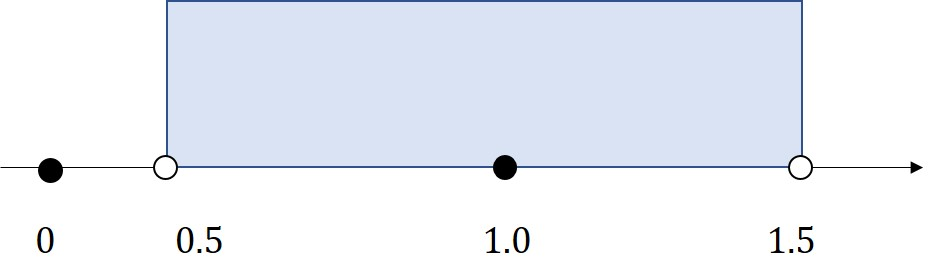
\includegraphics{vecindad}
\caption{Vecindad de centro $ 1 $ y radio $ 0.5 $}
\label{vecindad_im1}
\end{figure}
\newpage



\begin{thm}\label{vecindad_reducida}
	Una vecindad reducida es el conjunto de puntos de la recta real que satisfacen la siguiente desigualdad:\\
	\[ 0<|x-l|<\epsilon\]
		 
		 
\end{thm}
	Esta difiere de una vecindad en que su centro l no pertenece al intervalo. Ver figura (\ref{vecindad_reducida})



\begin{figure}[h]
	\centering
	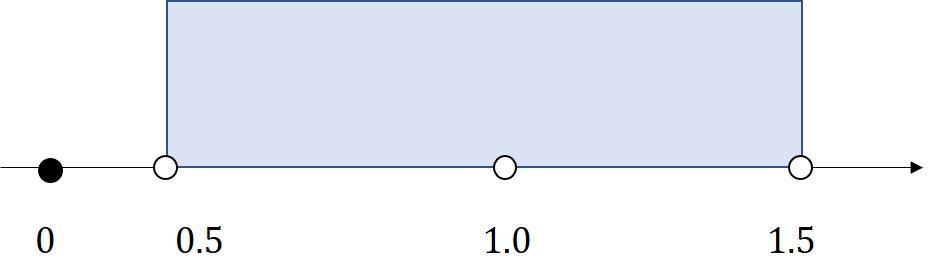
\includegraphics{vecindad_reducida}
	\caption{Vecindad reducida de centro $ 1 $ y radio $ 0.5 $}
	\label{vecindad_im2}
\end{figure}

\begin{thm}\label{limite_sucesiones}
	(Límite de una función por sucesiones)\\
		Se dice que $ l\in\mathbb{R} $ es l\'imite de la funci\'on $ f $ cuando $ x $ tiende al punto $ a $ si se verifica que:\\
	Para toda sucesión $ {x_{n}} $	tal que $ x_{n}\in X $, $ x_{n}\rightarrow a $ y $ x_{n}\neq a $ se cumple
	\[ f(x_{n})\rightarrow l \].
\end{thm}


\begin{ejemplo}
	Dada la función $ f(x)=2x^{2}+x-1 $. Se quiere saber \[ \lim\limits_{x\rightarrow0}f(x) .\]
	
	Sea $ {x_{n}} $ sucesión que tiende a cero, esto es $ x_{n}\rightarrow0 $.
	De la definición de límite por sucesiones, se tiene:
\[ \lim\limits_{x\rightarrow0}f(x)=\lim\limits_{n}f(x_{n})=l \]
\[ f(x_{n})=2x_{n}^{2}+x_{n}-1 \]
como $ x_{n} $ tinede a cero
\[ f(x_{n})\rightarrow2\cdot0+0-1=-1 \]

\end{ejemplo}

Usos más comunes de la  definición (\ref{limite_sucesiones}):\\
\begin{enumerate}
	\item Verificar la no existencia del límite de una función $ f $ en un punto $ x=a $.
	\item[i)]	Encontrar dos sucesiones $ {x_{n}^{(i)}} $ con $ (i=1,2) $ tales que: $ x_{n}^{(i)}\in X, \; x_{n}^{(i)}\rightarrow a, \; x_{n}^{(i)}\neq a $ y 
	\[ \lim\limits_{n}f(x_{n}^{(1)})\neq\lim\limits_{n}f(x_{n}^{(2)}). \]
	\item[ii)]	Encontrar una sucesión $ {x_{n}} $ tal que $ x_{n}\in X $, $ x_{n}\rightarrow a $, $ x_{n}\neq a $ y $ \lim\limits_{n}f(x_{n}) $ no existe.
\end{enumerate}

\begin{ejemplo}\label{ejemplo_signo_suceciones}
	Investique la existencia del límite de la función.
	\[ f(x)=sgn (x) \]
	Esta es la función signo de equis. La cual para se comporta de la siguiente forma:
	\[ sgn (x)=
\begin{cases}
	-1, & \mbox{$ x<0 $}\\
	0, &	\mbox{$ x=0 $}\\
	1, &	\mbox{$ x>0 $}
	
\end{cases}
\]
	 
	 Sea $ x_{n}^{(1)}=\dfrac{1}{n} $ y $ x_{n}^{(2)}=-\dfrac{1}{n} $ dos sucesiones. Como se puede apreciar una es mayor que cero $ n\in\mathbb{N} $ y la otra menor que cero. Entonces:
	 \[ sgn\left ( \dfrac{1}{n}\right )=1 \]
	 \[ sgn\left ( -\dfrac{1}{n}\right )=-1 \]
	 Se ha encontrado un par de sucesiones que tienden a cero y el límite de $ f(x_{n}) $ es distinto para ambas. Lo cual contradice la definición (\ref{limite_sucesiones}).
	 Por lo tanto en el punto $ x=0 $ la función signo de x, no tiene límite.
	 
	
	 
\end{ejemplo}

Estas propiedades se derivan de las propiedades de los límites de sucesiones.


\newtheorem{propiedad}{Propiedad}
\begin{propiedad}
Sean las funciones $ f,g:V^{*}(a)\rightarrow\mathbb{R} $ y supongamos que existen $ \lim\limits_{x\rightarrow a}f(x) $ y $ \lim\limits_{x\rightarrow a}g(x) $, entonces:\\
\begin{enumerate}
	\item[a)] 	$ \lim\limits_{x\rightarrow a}[f(x)\pm g(x)]=\lim\limits_{x\rightarrow a}f(x)\pm\lim\limits_{x\rightarrow a}g(x) $.
	
	
	\item[b)] 	$ \lim\limits_{x\rightarrow a}[f(x)\cdot g(x)]=\lim\limits_{x\rightarrow a}f(x)\cdot\lim\limits_{x\rightarrow a}g(x) $.
	
	
	\item[c)]	Si $ \lim\limits_{x\rightarrow a}g(x)\neq0 $ entonces $ \lim\limits_{x\rightarrow a}\dfrac{f(x)}{g(x)}=\dfrac{\lim\limits_{x\rightarrow a}f(x)}{\lim\limits_{x\rightarrow a}g(x)} $.
	
	
	\item[d)] 	Si $ \lim\limits_{x\rightarrow a}f(x)>0 $ entonces $ \lim\limits_{x\rightarrow a}\sqrt[k]{f(x)}=\sqrt[k]{\lim\limits_{x\rightarrow a}f(x)} $.
\end{enumerate}	
\end{propiedad}
	

\begin{thm}
	Sea $ f:X\rightarrow\mathbb{R} $ y $ x=a $ punto de \textsf{acumulación de $ X $}. Llamamos a $ l\in\Re $ límite por la derecha (por la izquierda) de $ f $ en el punto $ x=a $ si para todo $ {x_{n}} $ tal que $ x_{n}\in X $, $ x_{n}\rightarrow a $ y $ x_{n}>a $($ x_{n}<a $), si cumple que $ f(x_{n})\rightarrow l $ .
\end{thm}
\textbf{Notación}:\\
\[ \lim\limits_{x\rightarrow a+}f(x)=l\;\;\;\;\;\;\;\;\;\ \mbox{límite lateral derecho}.\]
\[ \lim\limits_{x\rightarrow a-}f(x)=l\;\;\;\;\;\;\;\;\;\ \mbox{límite lateral izquierdo}.\]

%\textbf{L\'imite de una funci\'on:}\\
%\textbf{Definici\'on}:\\ 


\begin{thm}
	\label{limite}

La funci\'on $ f $ tiende hacia el l\'imite l en $ x=a $, si y solo si, para todo $ \epsilon>0 $ existe alg\'un $ \delta>0 $ tal que, para todo $ x $, si  \[ 0<|x-a|<\delta \] 
 entonces
   \[ |f(x)-l|<\epsilon  \]
    y lo denotamos:\\

\[   \lim\limits_{x\rightarrow a}f(x)=l   \]
Se lee "l\'imite de $ f(x) $ cuando $ x $ tiende a a es igual a $ l $".\\
\end{thm}
(Esta definici\'on es conocida como la definici\'on $ \epsilon-\delta $ de l\'imite).\\
(tomada de pag. 34 CEM)	\\
\\
\newtheorem{teorema}{Teorema}
\begin{teorema}\label{Teorema_equivalencia-entre_definiciones_limite}
	Son equivalentes:\\
	\begin{enumerate}
		\item [(a)]	Para toda $ {x_{n}} $ tal que $ x_{n}\in X $, $ x_{n}\neq a $, $ x_{n}\rightarrow a $, se cumple $ f(x_{n})\rightarrow l $.
		
		
		\item [(b)]	Para todo $ \epsilon>0 $, existe $ \delta>0 $, tal que se $ x\in X $ y $ 0<|x-a|<\delta $, entonces $ |f(x)-l|<\epsilon $.
		
		
	\end{enumerate}
\end{teorema}	

\begin{thm}
	(Límite en el lenguaje de las vecindades)\\
	Para toda $ V_{\epsilon}(l) $, se encuentra $ V_{\delta}^{*}(a) $ tal que:\\
	\[ x\in X\cap V_{\delta}^{*}(a)\Rightarrow f(x)\in V_{\epsilon}(l) \]
	
	
\end{thm}

\begin{ejemplo}
	Sea $ f(x)=x^{2} $, calcula $ \lim\limits_{x\rightarrow0}f(x) $ usando la definición $ \epsilon-\delta $.\\
	\textbf{Respuesta}\\
	De la definión se tiene que dado un $ \epsilon>0 $ se puede encontrar alg\'un $ \delta>0 $ que este debe estar en funci\'on de $ \epsilon $, $ \delta=\delta(\epsilon) $, tal que:\\
	si	$ x\in X $ y $ 0<|x-a|<\delta $, entonces $ |f(x)-l|<\epsilon $.\\
	El $ l $ es lo que queremos buscar y verificar su unicidad. Como se va a usar la definici\'on $ \epsilon-\delta $, debemos tener presente que esta definici\'on se basa en el análisis geométrico. El cual se puede hacer con un previo conocimiento de la gráfica de la función. Ver en anexos figura (\ref{funciones algebraicas1}).\\
	Primero hay que preguntar:\\
	¿Está definida la función en $ x=1 $?\\
	Esto quiere decir que, en caso afirmativo, la función tendrá una imagen para $ x=1 $ en su conjunto de partida. Es fácil percatarse de que $ f(1)=1^{2}=1 $, por lo cual si está definida.\\
	
	\fbox{$ l=1 $ es el posible límite.}\\
	Sea un $ \epsilon>0 $, hay que verificar si el $ l=1 $ cumple con la definici\'on. Debemos encontrar alg\'un $ \delta>0 $, tal que $ |x^{2}-1|<\epsilon $, cuando $ 0<|x-1|<\delta $. Como se va a trabajar con vecindades pequeñas, supondremos que $ \delta<1 $.\\
	\newpage
	Entonces:\\
	\[ |x-1|<\delta \]
	\[ \Rightarrow0<1-\delta<x<1+\delta<3 \]
	Como $ \delta<1 $, será $ 1+\delta<2 $ y también $ 1+\delta<3 $, de ahí se tiene que que $  |x+1|<3 $.\\
	Por otro lado 
	\[ |x^{2}-1|=|x-1|\cdot|x+1|<3 \]
	por diferencia de cuadrados y la desigualdad antes analizada.\\
	Si 
	\[ |x^{2}-1|<\epsilon \]
	\[ \Rightarrow|x-1|\cdot|x+1|<\epsilon \]
	\[ \Rightarrow|x-1|<\dfrac{\epsilon}{|x+1|} \]
	\[ \Rightarrow|x-1|<\dfrac{\epsilon}{3} \]
	Entonces como se ve se puede encontrar algún $ \delta=\min\left \{1,\dfrac{\epsilon}{3}\right \} $.
	Por lo tanto el límite de $ f(x) $ cuando $ x $ tiende a cero es $ 1 $
	\[ \lim\limits_{x\rightarrow0}f(x)=1 \]
	\[ \lim\limits_{x\rightarrow0}x^{2}=1 \]	
\end{ejemplo}

Como se puede apreciar en la definición (\ref{limite}), la elección de $ \delta $ depende de la previa selección de $ \epsilon $. Por ende para demostrar la existencia del límite de una función, hay que probar que dado cualquier $ \epsilon>0 $, se puede encontrar un $ \delta>0 $, tal que:
\[ 	 0<|x-a|<\delta\Rightarrow |f(x)-l|<\epsilon  \]
\\
\textbf{Precedimiento para demostrar la existencia del límnite de una función usando la definición $ \epsilon-\delta $:}\\
\begin{enumerate}
	\item Se descompone $ |f(x)-l| $ en dos factores del tipo:
	\[ |f(x)-l|=|x-a|\cdot|g(x)| \]
	\item Se busca acotar o mayorar la funci\'on $ g(x) $ hallando dos números positivos $ \delta_{1} $ y $ M $ tal que:
	\[ 0<|x-a|<\delta_{1}\Rightarrow |g(x)|\leq M \]
	\item Elegido $ \delta_{1} $, se construye $ g(x) $ de la siguiente manera.\\
		Si $ 0<|x-a|<1 $, entonces 
		 \[ |x-a|\cdot|g(x)|=|f(x)-l|\leq|x-a|\cdot M \] 
		 luego, si $ |f(x)-l|<\epsilon $ por transitividad, sigue:
		 \[ |x-a|\cdot M<\epsilon \]
		 siempre que:
		 $ |x-a|<\dfrac{\epsilon}{M}=\delta_{2} $
		 
		 
		 \item $ \delta=\min(\delta_{1},\delta_{2} ) $.
\end{enumerate}
En resumen para demostrar que $ \lim\limits_{x\rightarrow a}f(x)=l $ tienen que ser ciertas todas las afirmaciones de este procedimiento.

\begin{ejemplo}
	Demostrar que $ \lim\limits_{x\rightarrow0}sgn(x)=0 $ es falsa usando la definici\'on $ \epsilon-\delta
	 $ (\ref{limite}).\\
	 \textbf{Respuesta:}\\
	 Ya se sabe que sucede gracias al ejemplo (\ref{ejemplo_signo_suceciones}). Supongamos que es cierta la afirmaci\'on para proceder por la vía de reducçión al absurdo.
	 \[ |sgn(x)-0|=|x-0|\cdot\left |\dfrac{sgn(x)-0}{x-0}\right |\]
	  \[ \Rightarrow |sgn(x)|=|x|\cdot\left |\dfrac{sgn(x)}{x}\right |\]
	  \[  \Rightarrow |sgn(x)|=|x|\cdot\left |\dfrac{1}{x}\right | \]
	  Si se fija $ \delta_{1}=1 $ y se tiene que:\\
	  
	  \fbox{$ |x|<1\Rightarrow\left|\dfrac{1}{x}\right |>1  $ }\\
	  que como se puede apreciar es una  señal, de que la definición no se cumplirá. Pues no se puede fijar un $ M $, que acote a $ g(x)=\dfrac{1}{x} $; cuando $ \delta 
	   $ decrece.\\
%	  Entonces si se fija un $ \epsilon=2 $
%	  \[ |sgn(x)|=|x|\cdot\left |\dfrac{sgn(x)}{x}\right |=1<2 \]
%	  lo cual implica que
%	  \[ |x|\cdot\left |\dfrac{sgn(x)}{x}\right |<2 \]
Ya que 	  
	  \[ |x|\cdot\left |\dfrac{1}{x}\right |<\epsilon \]
	  \[\Rightarrow |x|<\epsilon|x| \]
Solo se cumple para $ \epsilon>1 $ y no para todo $ \epsilon>0 $, que es lo que se dice en la definición.\\ Conradición!!\\
$ 0 $ no es el límite de $ sgn(x) $ en $ x=0 $.
\end{ejemplo}

%%%%%%%%%%%%%%%%%%%%%%%%%%%%%%%%%%%%%%%%%%%%%%%%%%%%%%%%%%%%%%%%%%%%%%%%%%%%%%%%%%%%%%%%%%%%%%%%%%%%%%%%%%%%%%%%%%%%%%%%%%%%%%%%%%%%%%%%%%%%%%%%%%%%%%%%%%%%%%%%%%%%%%%%%%%%%%%%%%%%%%%%%%%%%%%%%%%%%%%%%%%%%%%%%%%%%%%%%%%%%%%%%%%%%%%%%%%%%%%%%%%%%%%%%%%





\subsection{Continuidad de una funci\'on}

En la secci\'on anterior se calcula el límite usando la definición, lo cual es tedioso. Estos procedimientos antes mostrados son útiles para algunos casos específicos. Con el concepto de continuidad, que es más abarcador que el de límite, al derivar de este, se reduce el trabajo.\\
La idea intuitiva que hay detras del concepto de continuidad de una funci\'on, es la geométrica: es una función que puede ser representada por una curva que es posible dibujar sin levantar el lápiz.
%%%%%%%%%%%%%%%%%%%%%%%%%%%%%%%%%%%%%%%%%%%%%%%%%%%%%%%%%%%%%%%%%%%%%%%%%%%%%%%%%%%%%%%%%%%%%%%%%%%%%%%%%%%%%%%%%%%%%%%%%%%%%%%%%%%%%%%%



%\textbf{Continuidad de una función\\}
\[ f(x)=\begin{cases}
x\cdot\sin(\dfrac{\pi}{x}) & \mbox{$ x\neq0 $}\\
0 & \mbox{$ x=0 $}
\end{cases} \]
Con esta funci\'on sucede algo atípico, que motivó a la aparición de otro tipo de análisis más riguroso.\\
\begin{figure}[h]
	\centering
	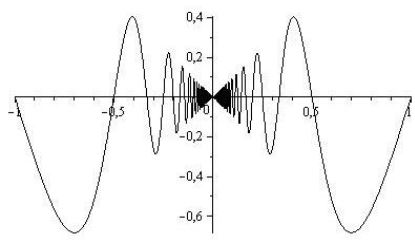
\includegraphics[width=7cm]{xsin_pix}
	\caption{}
	\label{xsin_pix}
\end{figure}
%\newpage

\begin{thm}\label{Continuidad_definicion_secilla}
	Sea una función real $ f $ con dominio $ X $ y un punto $ a\in X $, que a su vez está contenido en infinidad vecindades reducidas de $ a $. Se dice que la función $ f $ es continua en el punto $ a $ si se cumple que:
	\[ \lim\limits_{x\rightarrow a}f(x)=f(a). \]
\end{thm}


\textbf{Observaciones:}\\
La función f es continua en $ x=a $ si:\\
\begin{enumerate}
	\item Está definida en $ x=a $.
	\item Existe y es finito $ \lim\limits_{x\rightarrow a}f(x) $.
	\item $ \lim\limits_{x\rightarrow a}f(x)=f(a) $.
\end{enumerate}
De no cumplirse alguno de estos puntos estamos en presencia de un punto de discontinuidad.\\
 La continuidad de una función $ f $ en un punto a es una \textsl{característica loca}l, es decir,
 depende solo del comportamiento de $ f $ en una vecindad suficientemente pequeña de $ x=a $.

Hay que tener en cuenta que hay tantas definiciones de continuidad como definiciones de límite hay. Pero la m\'as general es esta (\ref{Continuidad_definicion_secilla}).\\
%%%%%%%%%%%%%%%%%%%%%%%%%%%%%%%%%%%%%%%%%%%%%%%%%%%%%%%%%%%%%%%%%%%%%%%%%%%%%%%%
\textbf{Caracterización:}\\
$ f $ es continua en un dominio si es continua en cada punto de ese dominio.\\
\begin{propiedad}
	Todas las funciones elementales son continuas en su dominio de definición.\\	
\end{propiedad}
%%%%%%%%%%%%%%%%%%%%%%%%%%%%%%%%%%%%%%%%%%%%%%%%%%%%%%%%%%%%%%%%%%%%%%%%%%%%%%%1
Ver Análisis Matemático I del CEM (Libro de Texto) e ISPJAE.\\

%%%%%%%%%%%%%%%%%%%%%%%%%%%%%%%%%%%%%%%%%%%%%%%%%%%%%%%%%%%%%%%%%%%%%%%%%%%%%%%%%%%%%%%%%%%%%%%%%%%%%%%%%%%%%%%%%%%%%%%%%%%%%%%%%%%%%%%%%%%%%%%%%%%%%%%%%%%%%%%%%%%%%%%%%%%%%%%%%%%%%%%%%%%%%%%%%%%%%%%%%%%%%%%%%%%%%%%%%%%%%%%%%%%%%%%%%%%%%%%%%%%%%%%%%%%
\begin{ejemplo}
	Dada $ f(x)= \ln x $ analice su continuidad en $ x=1 $.\\
	*\textbf{Recordatorio}: $ \ln x $ es una función logarítmica de base $ e $. Conocida como logaritmo natural o neperiano $ \log_{e}x =\ln x$.\\
	También se tiene que\\
\begin{eqnarray}
e^{x}=y\\
\ln (e^{x})=\ln y\\
x=\ln y
\end{eqnarray}
Entonces \[ 1=\ln e \]
Todo esto por propiedad de los logaritmos.\\

\end{ejemplo}


\textbf{Notación:}
\[ f,g\in\textsf{C}(E) \]
Quiere decir: las funciones $ f, g $ pertenecen al conjunto de las funciones continuas en $ E $, es decir, son continuas en todo $ E $.\\

\textbf{Propiedades de las funciones continuas:}
El estudio de estas propiedades facilitar\'ia en gran medida, la determinación del dominio de continuidad de innumerables funciones. Tener en cuenta que la continuidad es una propiedad local.
\begin{propiedad}\label{propiedad1_continuidad}
	Si las funciones $ f $ y $ g $ son continuas en $ a $, entonces, también son continuas en $ a  $ las funciones $ f\pm g $, $ f\cdot g $, $ f/g $ en este último para $ g(a)\neq0 $.
\end{propiedad}
\begin{center}
	\textbf{¿Qué usos tiene esta propiedad?}
\end{center}
Antes de todo hay que percatarse de que estas propiedades se derivan de las de límite. Los usos estan en propiedades derivadas de la (propiedad \ref{propiedad1_continuidad}). Aquí se puede ver con la linealidad.
\begin{propiedad}\label{linealidad_propiedad}
	Dada $ f,g\in\textsf{C}(E)\Rightarrow\alpha f+\beta g \in\textsf{C}(E) $ para cualesquiera $ \alpha, \beta\in\mathbb{R} $.
\end{propiedad}
Esta propiedad es conocida cmo la linealidad.\\
\textbf{*Notación:}\\
$ \Rightarrow $ significa implicación. Por otro lado, $ \alpha f+\beta g $ es la combinaci\'on lineal de dos funciones. Producto de una constante por una función sumado por el producto de otra función multiplicada por una constante.\\
\begin{ejemplo}
	Es evidente que $ f(x)=x $ es continua en todo $ \mathbb{R} $, entonces $ g(x)=f^{2}(x)=x^{2} $ y $ x^{2}+2x $ tambi\'en son continuas en todo $ \mathbb{R} $. Por cumplir las pripiedades antes enunciadas.\\
\end{ejemplo}

\begin{propiedad}
	(Continuidad de la función compuesta)\\
	Sean la función $ y=f(x) $, definida en $ V(a) $ y continua en $ a $ y la función $ z=g(y) $ definida en $ V(b) $ y continua en $ b $, donde $ b=f(a) $. Entonces, la función compuesta $ g\circ f $ es continua en $ a $.
	 \begin{equation}
	\lim\limits_{x\rightarrow a}g(f(x))=g\left  (\lim\limits_{x\rightarrow a}f(x)\right  )
	\end{equation} 
	
\end{propiedad}
\begin{propiedad}
	(Conservación del signo)\\
	Supongamos que la función $ f $ es continua en el punto $ a $ y $ f(a)\neq0 $, entonces exite alguna $ V(a) $ tal que $ sgn(f(x))=sgn(f(a)) $ para $ x\in V(a) $.
\end{propiedad}

\begin{figure}[h]
	\centering
	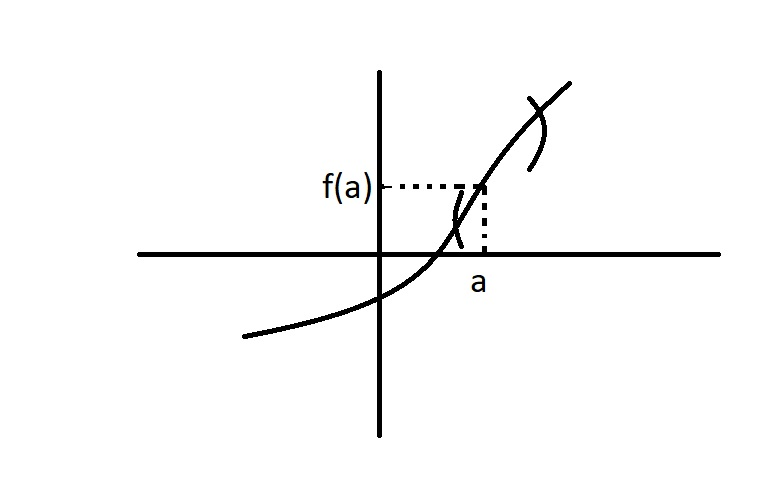
\includegraphics[width=7cm]{Conservacion_signo}
	\caption{En la vecindad de $ a $ se conserva el signo, positivo en este caso.}
	\label{Conservacion_signo}
\end{figure}
\begin{propiedad}
	(Acotación local)\\
	Sea la funci\'on definida en el conjunto $ X $. Si $ f $ es continua en $ a\in X $, entonces exite una vecindad de $ a $, $ V(a) $ tal que $ f $ esta acotada en $ V(a)\cap X $.
\end{propiedad}
\begin{ejemplo}
	Analice la continuidad de
	\[ f(x)=\dfrac{1}{\sin x}-1  \;\;\;\;\;\;\;\;\;\;\;\;\;\;\; \hbox{en $ (0,\pi) $}.\]
\end{ejemplo}




%%%%%%%%%%%%%%%%%%%%%%%%%%%%%%%%%%%%%%%%%%%%%%%%%%%%%%%%%%%%%%%%%%%%%%%%%%%%%%%%%%%%%%%%%%%%%%%%%%%%%%%%%%%%%%%%%%%%%%%%%%%%%%%%%%%%%%%%%%%%%%%%%%%%%%%%%%%%%%%%%%%%%%%%%%%%%%%%%%%%%%%%%%%%%%%%%%%%%%%%%%%%%%%%%%%%%%%%%%%%%%%%%%%%%%%%%%%%%%%%%%%%%%%%%%%%%%%%%%%%
\subsection{Tipos de discontinuidades}
Cuando una función no es continua, no cumple con (\ref{Continuidad_definicion_secilla}), es decir es discontinua en el punto en cuesti\'on y por tanto si ese punto pertenece a su dominio en ese dominio.\\
\textbf{Tipos de discontinuidades:}\\
Existen tres tipos de discontinuidades, si la función $ f $ cumple que en $ x=a $:
\begin{enumerate}
	\item Evitable: $ f(a+)=f(a-)=L $ y $ f(a) $ no existe o es distinto de $ L $.
	\item Salto finito: si $ f(a+) $ y $ f(a-) $ existen y son finitos, pero $ f(a+)\neq f(a-) $
	\item Salto infinito: si $ f(a+) $ o $ f(a-) $ es $ \infty $.
\end{enumerate}

Son muchas las variedades de funciones discontinuas. Con la composici\'on de funciones elementales resultan unos casos:
\begin{enumerate}
	\item $ f(x)=\dfrac{1}{x-a} +b $ en $ x=a $ la discontinuidad es de salto infinito.(Ver (\ref{modulo1sobrex}))
	\item $ f(x)=\dfrac{\sin x}{x} $ en $ x=0 $ la discontinuidad es evitanble.
	\item $ f(x)=sgn(x) $, es salto finito. (Ver (\ref{funcion_signo_x}))
\end{enumerate}
\begin{figure}[h]
	\centering
	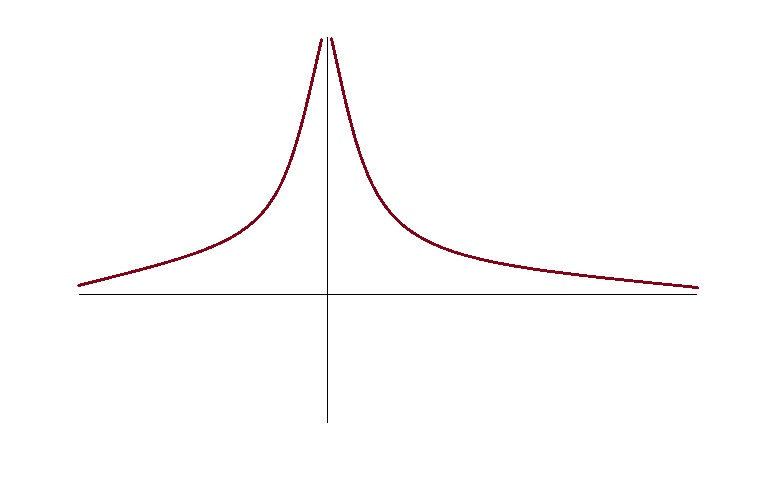
\includegraphics[width=7cm]{modulo1sobrex}
	\caption{Funci\'on  módulo de proporcionalidad inversa}
	\label{modulo1sobrex}
\end{figure}
%%%%%%%%%%%%%%%%%%%%%%%%%%%%%%%%%%%%%%%%%%%%%%%%%%%%%%%%%%%%%%%%%%%%%%%%%%%%%%%%%%%%%%%%%%%%%%%%%%%%%%%%%%%%%%%%%%%%%%%%%%%%%%%%%%%%%%%%%%%%%%%%%%%%%%%%%%%%%%%%%%%%%%%%%%%%%%%%%%%%%%%%%%%%%%%%%%%%%%%%%%%%%%%%%%%%%%%%%%%%%%%%%%%%%%%%%%%%%%%%%%%%%%%%%%%%%%%%%%%%%%%%%%%%%%%%
\begin{figure}[h]
	\centering
	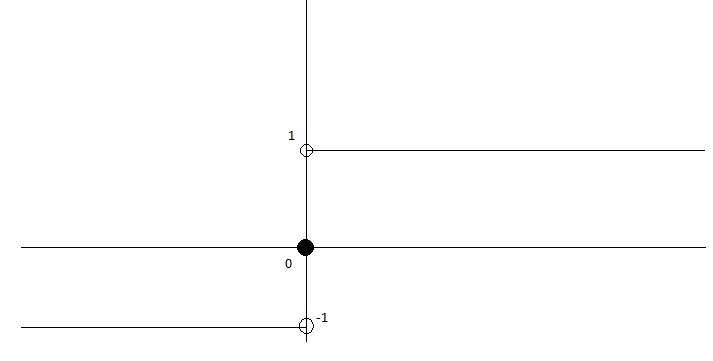
\includegraphics[width=7cm]{funcion_signo_x}
	\caption{Función signo de $ x $}
	\label{funcion_signo_x}
\end{figure}
La mayoría de las funciones con las que estamos familiarizados son muy bondadozas. Estas son continuas y derivables en todo su dominio, salvo una cantidad limitada de puntos. Pero se presenta excepciones como la función de Dirichlet
\[ D(x)=\begin{cases}
1 & \mbox{$ x\in\mathbb{Q} $}\\
0 & \mbox{$ x\in\mathbb{I} $}
\end{cases} \]

%\textbf{Notación:}\\
%$ f(a+)=\lim\limits_{x\rightarrow a+}f(x)$ l\'imite lateral derecho.\\
%$  f(a-)=\lim\limits_{x\rightarrow a-}f(x) $  l\'imite lateral izquierdo.\\

%%%%%%%%%%%%%%%%%%%%%%%%%%%%%%%%%%%%%%%%%%%%%%%%%%%%%%%%%%%%%%%%%%%%%%%%%%%%%%%%%%%%%%%%%%%%%%%%%%%%%%%%%%%%%%%%%%%%%%%%%%%%%%%%%%%%%%%%%%%%%%%%%%%%%%%%%%%%%%%%%%%%%%%%%%%%%%%%%%%%%%%%%%%%%%%%%%%%%%%%%%%%%%%%%%%%%%%%%%%%%%%%%%%%%%%%%%%%%%%%%%%%%%%%%%%%%%%%%%%%%%%%%%%%%%%%%%%%%%%%%%%%%%%%%%%%%%%%%%%%%%%%%%%%%%%%%%%%%%%%%%%%%%%%%%%%%%%%%%%%%%%%%%%%%%%%%%%%%%%%%%%%%%%%%%%%%%%%%%%%%%%%%%%



\subsection{Infinitos e infinit\'esimos}
%%%%%%%%%%%%%%%%%%%%%%%%%%%%%%%%%%%%%%%%%%%%%%%%%%%%%%%%%%%%%%%%%%%%%%%%%%%%%%%%%%%%%%%%%%%%%%%%%%%%%%%%%%%%%%%%%%%%%%%%%%%%%%%%%%%%%%%%%%%%%%%%%%%%%%%%%%%%%%%%%%%%%%%%%%%%%%%%%%%%%%%%%%%%%%%%%%%%%%%%%%%%%%%%%%%%%%%%%%%%%%%%%%%%%%%%%%%%%%%%%%%%%%%%%%%%%%%%%%%%%%%%%%%%%%%%%
El estudio de los límites de ciertas funciones ha demostrado la existencia de algunas que decrecen (crecen) indefinidamente. Estas tienen límite, en unos casos cero, en otros el infinito.\\
\begin{thm}
	El conjunto formado por los números reales y el objeto $ \infty $, punto del infinito, es conocido como la recta real ampliada o recta real extendida .
\[ \overline{\mathbb{R}}=[-\infty,+\infty]=\mathbb{R}\cup\{-\infty\}\cup\{\infty\} \]
\end{thm}	
La importancia de esta definición está en el hecho de que ya no habrá que decir que el límite no existe en $ \mathbb{R} $. Porque se estará calculando este en el conjunto de los reales ampliados $ \overline{\mathbb{R}} $.\\
\textbf{Función infinitesimal:}\\
En él se definen las siguientes operaciones:\\
\begin{enumerate}\label{operaciones_infty}
	\item $ x+\infty=\infty+x=\infty $, $ \forall x\in\mathbb{R} $.
	\item $ x-\infty=-\infty+x=-\infty $, $ \forall x\in\mathbb{R} $.
	\item $ x\cdot(\pm\infty)=(\pm\infty)\cdot x=\pm\infty $, $ \forall x\in\mathbb{R}; x>0 $.
	\item $ x\cdot(\mp\infty)=(\mp\infty)\cdot x=\pm\infty $, $ \forall x\in\mathbb{R}; x<0 $.
	\item $ (+\infty)+(+\infty)=(+\infty)(+\infty)=(-\infty)(-\infty)=+\infty $.
	\item $ (-\infty)+(-\infty)=(+\infty)(-\infty)=-\infty $.
	\item $ \dfrac{x}{\infty}=0 $.
\end{enumerate}
%x+∞=∞+x=∞		∀x∈ R
%x-∞=-∞+x=-∞		∀x∈ R
%x⋅(±∞)=(±∞)⋅x=±∞		∀x∈ R;x>0
%x⋅(∓∞)=(∓∞)⋅x=∓∞		∀x∈ R;x<0
%(+∞)+(+∞)=(+∞)(+∞)=(-∞)(-∞)=+∞		
%(-∞)+(-∞)=(+∞)(-∞)=-∞		
%x/∞=0					∀x∈ R

\begin{thm}
La función $ \alpha=\alpha(x) $ se denomina infinitamente pequeña o infinitesimal para $ x\rightarrow a $ si $ \lim\limits_{x\rightarrow a}\alpha(x)=0 $.\\
\end{thm}
\begin{teorema}
%\textbf{Teorema:}\\
La suma  de dos infinitesimales para $ x\rightarrow a $ es un infinitesimal para $ x\rightarrow a $.\\	
\end{teorema}



\begin{teorema}
El producto de un infinitésimo por una función acotada en un  entorno de $ x=a $ es un infinitésimo.\\
\end{teorema}


\newtheorem{corolario}{Corolario:}
\begin{corolario}
El producto de dos infinitesimales es un infinitesimal.\\
\end{corolario}

%\newpage


\textbf{Función infinitamente grande:}
\begin{thm}
La función $ \beta=\beta(x) $ es infinitamente grande o infinita para $ x\rightarrow a $ si $ \lim\limits_{x\rightarrow a}\beta(x) =\infty$.
	
\end{thm}
%\textbf{Teorema:}\\
\begin{teorema}
Si $ \alpha(x) $ es un infinitesimal para $ x\rightarrow a $ y $ \alpha(x)\neq 0 $ para todo $ x\in \Re $, entonces $ \beta(x)=1/\alpha(x) $ es un infinito.\\
	
\end{teorema}
\textbf{Demostración:}
Como $ \alpha(x) $ es un infinitesimal para $ x\rightarrow a $, para todo $ \epsilon>0 $ existe $ \delta>0 $ tal que si $ 0<|x-a|<\delta $ entonces $ |\alpha(x)|<\epsilon $\\
Que se puede escribir como
\[  \left|\frac{1}{\alpha(x)} \right|<\frac{1}{\epsilon}  \]



\begin{ejemplo}
	A continuación algunos casos:\\
\begin{enumerate}
	\item $ f(x)=\frac{1}{x} \;\;\;\;\;\;\;\;\;\;\;\;\;\;	 \lim\limits_{x\rightarrow\infty}f(x)=0 $
	\item $	G(x)=\frac{1}{x}+\sin(x) \;\;\;\;\;\;\;\;\;\;\;\;\;\;	 \lim\limits_{x\rightarrow 0}G(x)=0 $
	\item $	h(x)=x\cos(x)	\;\;\;\;\;\;\;\;\;\;\;\;\;\;	\lim\limits_{x\rightarrow 0}h(x)=0 $
	
\end{enumerate}
%
\end{ejemplo}
%%%%%%%%%%%%%%%%%%%%%%%%%%%%%%%%%%%%%%%%%%%%%%%%%%%%%%%%%%%%%%%%%%%%%%%%%%%%%%%%%%%%%%%%%%%%%%%%%%%%%%%%%%%%%%%%%%%%%%%%%%%%%%%%%%%%%%%%%%%%%%%%%%%%%%%%%%%%%%%%%%%%%%%%%%%%%%%%%%%%%%%%%%%%%%%%%%%%%%%%%%%%%%%%%%%%%%%%%%%%%%%%%%%%%%%%%%%%%%%%%%%%%%%%%%%%%%%%%%%%%%%%%%%%%%%%%%%%%%%%%%%%%%%%%%%%%%%%%%%%%%%%%%%%%%%%%%%%%%%%%%%%%%%%%%%%%%%%%%%%%%%%%%%%%%%%%%%%%%%%%%%%%%%%%%%%%%%%%%%%%%%%%%%
\subsubsection{Infitésimos equivalentes}

Estos surgen a partir de la observaci\'on de que dos funciones infinitamente pequeñas tienden a cero en el mismo punto. 
\\

Límites fundamentales:
\begin{enumerate}
	\item El límite fundamental trigonom\'etrico $ \lim\limits_{x\rightarrow0}\dfrac{\sin x}{x}=1 $.
	
	\item El límite fundamental algebraico $ \lim\limits_{x\rightarrow\infty}\left (1+\dfrac{1}{x}\right )^{x}=e $
\end{enumerate}

%\newtheorem{definicion}{Definición:}
\begin{thm}
	Sean $ \alpha $ y $ \beta $ infinitesimales para $ x=a $. Si
	\[ \lim\limits_{x\rightarrow a}\dfrac{\alpha(x)}{\beta(x)}=L\neq0 \]
	Entonces $ \alpha $ y $ \beta $  son infinitesimales del mismo orden.
	
\end{thm}

\begin{thm}
	Si $ \alpha $ y $ \beta $ son infinitesimales para $ x\rightarrow a $ y $ \lim\limits_{x\rightarrow a}\dfrac{\alpha(x)}{\beta(x)}=1 $
	Entonces $ \alpha $ y $ \beta $  son infinitesimales equivalentes.\\
	Se designa $  \alpha(x)\sim\beta(x) $  cuando $ x\rightarrow a $.
	
\end{thm}

Algunos infinitesimales equivalentes cuando $ x\rightarrow0 $:\\
\begin{enumerate}\label{infinitesimos_tabla}
	\item $ \sin(x)\sim x $
	\item $ \tan x \sim x $
	\item $ \arcsin x\sim x $
	\item $ \ln(1+x)\sim x $
	\item $ (1+x)^{\alpha}-1\sim\alpha x $
	\item $ e^{x}-1\sim x $
	\item $ 1-\cos x\sim\dfrac{x^{2}}{2} $
	
%	\newtheorem{ejemplo}{Ejemplo:}
	\begin{ejemplo}
		Calcular $ \lim\limits_{x\rightarrow0}\dfrac{\ln(\sin x)}{\tan x^{2}} $.\\
		\textbf{Respuesta:}\\
		Hay que tener en cuenta que por lo general, los infinitésimos equivalentes son usados para resolver ejercicios con indeterminaciones del tipo $ \dfrac{0}{0} $ o $ \dfrac{\infty}{\infty}
		$.
		\begin{equation}
		\lim\limits_{x\rightarrow0}\dfrac{\ln(\sin x)}{\tan x^{2}}
		\end{equation}
		aplicando propiedades de los límites, tenemos:
		\begin{equation}
		=\dfrac{\lim\limits_{x\rightarrow0}\ln(\sin x)}{\lim\limits_{x\rightarrow0}\tan x^{2}}
		\end{equation}
		\begin{equation}
		=\dfrac{\ln(\sin \lim\limits_{x\rightarrow0}x)}{\tan \lim\limits_{x\rightarrow0}x^{2}}=0/0
		\end{equation}
		que se puede apreciar una indetermincación del tipo $ \dfrac{0}{0} $.
		Aplicando infinitésimos, es la forma de solucionarla:
		\begin{equation}
		\lim\limits_{x\rightarrow0}\dfrac{\ln(\sin x)}{\tan x^{2}}
		\end{equation}
		Con la equivalencia 1 y 2 de (\ref{infinitesimos_tabla}), se tiene
		\begin{equation}
		=\lim\limits_{x\rightarrow0}\dfrac{\ln(x)}{ x^{2}}
		\end{equation}
		si se suma y resta $ 1 $ para aplicar el 5 de (\ref{infinitesimos_tabla})
		\begin{equation}
		=\lim\limits_{x\rightarrow0}\dfrac{\ln(1+x-1)}{ x^{2}}
		\end{equation}
		\begin{equation}
		=\lim\limits_{x\rightarrow0}\dfrac{x}{ x^{2}}
		\end{equation}
		\begin{equation}
		=\lim\limits_{x\rightarrow0}\dfrac{1}{ x}=\infty
		\end{equation}
	\end{ejemplo}
	
	
\end{enumerate}
\subsubsection{Límites fundamentales}

\textbf{Límite fundamental trigonométrico}\\
\[ \lim\limits_{x\rightarrow0}\dfrac{\sin x}{x}=1 \]
\textbf{Demostración:}\\
Cuando comenzamos a calcular el límite, notamos que
\[ \lim\limits_{x\rightarrow0}\dfrac{\sin x}{x}=\dfrac{0}{0} \]
lo cual es una indeterminación.\\
De un análisis geométrico (\ref{limite_fundamental}) tenemos,
\begin{equation}
 \sin x< x<\tan x 
\end{equation}

\begin{figure}[h]
	\centering
	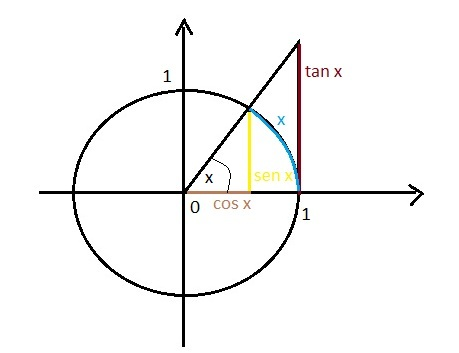
\includegraphics[width=7cm]{limite_fundamental}
	\caption{Circunferencia de radio 1}
	\label{limite_fundamental}
\end{figure}
Si se divide por $ \sin x $
\begin{equation}
 \dfrac{\sin x}{\sin x}< \dfrac{x}{\sin x}<\dfrac{\tan x }{\sin x}
\end{equation}
\begin{equation}
1< \dfrac{x}{\sin x}<\dfrac{1}{\cos x}
\end{equation}
Haciendo transformaciones algebraicas
\begin{equation}
\cos x<\dfrac{\sin x}{x}<1
\end{equation}
Pasando al límite, se procede a calcular el límite de cada elemento de la desigualdad, de esta el único de interés es 
\[ \lim\limits_{x\rightarrow0+}\cos x =1 \]
\begin{equation}
\lim\limits_{x\rightarrow0}\cos x
<\lim\limits_{x\rightarrow0}\dfrac{\sin x}{x}
<\lim\limits_{x\rightarrow0}1
\end{equation}
\begin{equation}
1<\lim\limits_{x\rightarrow0}\dfrac{\sin x}{x}<1
\end{equation}
Entonces por el criterio del emparedado se tiene que $ \lim\limits_{x\rightarrow0}\dfrac{\sin x}{x}=1 \boxtimes$\\

\begin{thm}
	Se denomina número $ "e" $ a:
	\[ e=\lim\limits_{n\rightarrow\infty}\left (1+\dfrac{1}{n}\right )^{n} \]
	con $ n\in\mathbb{N} $\\
	$ e $ es un número irracional, también conocido como número de Euler.
	
\end{thm}
\textbf{Límite fundamental algebraico:}\\
	\[ \lim\limits_{x\rightarrow\infty}\left (1+\dfrac{1}{x}\right )^{x}=e \]
	con $ x\in\mathbb{R} $\\
\textsf{Notar la diferencia en este caso $ x $ es real.}\\
\textbf{Demostración:}\\
Supongamos que:
\[ x\rightarrow+\infty \]
entonces se va a cumplir
\[ n\leq x\leq n+1 \]
\[ \dfrac{1}{n}\geq\dfrac{1}{x}\geq\dfrac{1}{n+1} \]
\begin{equation}
\left ( 1+\dfrac{1}{n}\right )^{n+1}
\geq \left ( 1+\dfrac{1}{x}\right )^{x}
\geq \left ( 1+\dfrac{1}{n+1}\right )^{n}
\end{equation}
Hallando los límites de las cotas
\begin{equation}
\lim\limits_{n\rightarrow\infty}\left ( 1+\dfrac{1}{n}\right )^{n+1}
=\lim\limits_{n\rightarrow\infty}\left ( 1+\dfrac{1}{n}\right )^{n}\cdot\lim\limits_{n\rightarrow\infty}\left ( 1+\dfrac{1}{n}\right )
=e
\end{equation}
Por otro lado
\begin{equation}
\lim\limits_{n\rightarrow\infty}\left ( 1+\dfrac{1}{n+1}\right )^{n}
=\dfrac{\lim\limits_{n\rightarrow\infty}\left ( 1+\dfrac{1}{n+1}\right )^{n+1}}{\lim\limits_{n\rightarrow\infty}\left ( 1+\dfrac{1}{n+1}\right )}
=e
\end{equation}
Y por el criterio del emparedado se tiene que 
	\[ \lim\limits_{x\rightarrow\infty}\left (1+\dfrac{1}{x}\right )^{x}=e \]
	$ \blacksquare $
	\\
	Lo mismo sucede con $ x\rightarrow-\infty. $\\


\textbf{Generalización con respecto al límite fundamental algebraico:}\\
Si $ f(x) \rightarrow0 $ y $ g(x)\rightarrow0 $ cuando $ x\rightarrow x_{0} $, entonces:
\[ \lim\limits_{x\rightarrow x_{0}}\left (1+f(x)\right )^{g(x)}  \]
\[ =\lim\limits_{x\rightarrow x_{0}}e^{g(x)\ln(1+f(x))} \]
\[ =e^{\lim\limits_{x\rightarrow x_{0}}f(x)\cdot g(x)} \]
pues si $ f(x)\rightarrow0\Rightarrow\ln(1+f(x))\sim f(x) $.




\subsubsection{As\'intotas de una funci\'on}
\begin{thm}
	Una recta se llama \textsf{asíntota de una curva} si la distancia de un punto $ M $ de la curva a la recta tiende a cero, cuando este punto se aleja infinitamente sonbre la curva.
\end{thm}

\textbf{Asíntota horizontal}\\
Son asíntotas paralelas al eje $ "x" $.\\


\textbf{Asíntota vertical}\\
Son asíntotas paralelas al eje $ "y" $. Se determinan buscando valores finitos para los cuales la función en cuestión tiene límite infinito ($ \lim\limits_{x\rightarrow x_{0}}f(x)=\infty $).\\

\textbf{Asíntota no vertica (oblicua)}\\
Es la asíntota que no es paralela a ningún eje. Es una recta de la forma $ y=mx+b $\\
\[ m=\lim\limits_{x\rightarrow\infty}\dfrac{f(x)}{x} \]
\[ b=\lim\limits_{x\rightarrow\infty}(f(x)-mx) \]

\begin{ejemplo}
	Sea $ f(x)=\dfrac{1}{x-1} $
	Esta función tiene una asíntota horizontal en $ y=0 $ y una vertical el $ x=1 $.
\end{ejemplo}

\begin{ejemplo}
	Sea
	\[ f(x)=\dfrac{x^{2}+2x-1}{x} \]
	para calcular sus as\'intotas oblicuas
	\begin{equation}
	m=\lim\limits_{x\rightarrow\infty}\dfrac{x^{2}+2x-1}{x}\cdot\dfrac{1}{x}
	\end{equation}
	\begin{equation}
		m=\lim\limits_{x\rightarrow\infty}\dfrac{x^{2}+2x-1}{x^{2}}=1
	\end{equation}
	\begin{equation}
		b=\lim\limits_{x\rightarrow\infty}\left (\dfrac{x^{2}+2x-1}{x}-x\right )
	\end{equation}
	\begin{equation}
	b=\lim\limits_{x\rightarrow\infty}(x-x+2x-\dfrac{1}{x})=2
	\end{equation}
\end{ejemplo}



%%%%%%%%%%%%%%%%%%%%%%%%%%%%%%%%%%%%%%%%%%%%%%%%%%%%%%%%%%%%%%%%%%%%%%%%%%%%%%%%%%%%%%%%%%%%%%%%%%%%%%%%%%%%%%%%%%%%%%%%%%%%%%%%%%%%%%%%%%%%%%%%%%%%%%%%%%%%%%%%%%%%%%%%%%%%%%%%%%%%%%%%%%%%%%%%%%%%%%%%%%%%%%%%%%%%%%%%%%%%%%%%%%%%%%%%%%%%%%%%%%%%%%%%%%%%%%%%%%%%%%%%%%%%%%%%%%%%%%%%%%%%%%%%%%%%%%%%%%%%%%%%%%%%%%%%%%%%%%%%%%%%%%%%%%%%%%%%%%%%%%%%%%%%%%%%%%%%%%%%%%%%%%%%%%%%%%%%%%%%%%%%%%%


\subsection{Formas indeterminadas. Regla de Leibniz.}

\textbf{Formas indeterminadas:}\\
 
\begin{enumerate}\label{formasIndeterminadas}
	\item $ \frac{\infty}{\infty} $
	\item $ \frac{0}{0} $
	\item $ 0\cdot \infty $
	\item $ 0^{0} $
	\item $ \infty^{o} $
	\item $ 1^{\infty} $
	\item $ \infty-\infty $
\end{enumerate}
Prestarle atención a las operaciones entre infinitos (\ref{operaciones_infty}) y comparar con estas. Se puede notar que el c\'alculo del límite que en los casos usuales se resume a la aplicación de la propiedad correspondiente y evaluar en el punto en cuestión; no es solo eso, sino el resumen del comportamiento de la función en la vecindad del punto.\\
\begin{center}
\textbf{Regla de Leibniz}\\	
\end{center}

\begin{thm}
	Sea $ P(x) $ un polinomio de grado $ n $ y $ Q(x) $, de grado $ m $ :\\
	\[ P(x)=a_{n} x^{n}+...+a_{1} x+a_{0} \]
	\[ Q(x)=b_{m} x^{m}+...+b_{1} x+b_{0} \]
	\[ \lim\limits_{x\rightarrow\infty} \frac{P(x)}{Q(x)}=
	\begin{cases}
	0, & \mbox{$ n<m $} \\
	\frac{a_{n}}{b_{m}}, & \mbox{ $ n=m $}\\
	\infty, & \mbox{ $ n>m $}
	\end{cases}
	\]
		
\end{thm}

\textbf{Demostración}\\
La fracción a la que le estamos calculando el límite es\\
\[ \frac{P(x)}{Q(x)}=\frac{a_{n} x^{n}+...+a_{1} x+a_{0}}{b_{m} x^{m}+...+b_{1} x+b_{0}} \]
Que es equivalente a:\\
\[ \frac{\frac{a_{n} x^{n}+...+a_{1} x+a_{0}}{x^{m}}}{\frac{b_{m} x^{m}+...+b_{1} x+b_{0}}{x^{m}}}= 
\frac{\frac{a_{n} x^{n}}{x^{m}}+...+\frac{a_{1} x}{x^{m}}+\frac{a_{0}}{x^{m}}}{\frac{b_{m} x^{m}}{x^{m}}+...+\frac{b_{1} x}{x^{m}}+\frac{b_{0}}{x^{m}}}
\]
Todo depende del témino\\
\[ \dfrac{x^{n}}{x^{m}}=x^{n-m} \]
Calculádole el límite a esta última expresión se tiene que:\\
\[ \lim\limits_{x\rightarrow\infty}\dfrac{x^{n}}{x^{m}}=\lim\limits_{x\rightarrow\infty}x^{n-m}=\begin{cases}
0, & \mbox{$ n < m $} \\
1, & \mbox{$  n=m $}\\
\infty, &  \mbox{$ n>m $}\\
\end{cases}
\]


La demostración se completa con el cálculo del resto de los límites de la expresión, lo cual queda propuesto.\\



%%%%%%%%%%%%%%%%%%%%%%%%%%%%%%%%%%%%%%%%%%%%%%%%%%%%%%%%%%%%%%%%%%%%%%%%%%%%%%%%%%%%%%%%%%%%%%%%%%%%%%%%%%%%%%%%%%%%%%%%%%%%%%%%%%%%%%%%%%%%%%%%%%%%%%%%%%%%%%%%%%%%%%%%%%%%%%%%%%%%%%%%%%%%%%%%%%%%%%%%%%%%%%%%%%%%%%%%%%%%%%%%%%%%%%%%%%%%%%%%%%%%%%%%%%%%%%%%%%%%%%%%%%%%%%%%%%%%%%%%%%%%%%%%%%%%%%%%%%%%%%%%%%%%%%%%%%%%%%%%%%%%%%%%%%%%%%%%%%%%%%%%%%%%%%%%%%%%%%%%%%%%%%%%%%%%%%%%%%%%%%%%%%%
\subsection{Ejercicios Resueltos}

%%%%%%%%%%%%%%%%%%%%%%%%%%%%%%%%%%%%%%%%%%%%%%%%%%%%%%%%%%%%%%%%%%%%%%%%%%%%%%%%%%%%%%%%%%%%%%%%%%%%%%%%%%%%%%%%%%%%%%%%%%%%%%%%%%%%%%%%%
\begin{enumerate}
	\item Dadas las siguientes funciones %Pregunta1
		\begin{enumerate}
			\item[a)]$  y=x^{3}+5  $
			\item[b)] $ x^{2}+y^{2}=9 $ 
			\item[c)] $ \begin{cases}
			x=t+1\\
			y=t+2
			\end{cases} $ 
		\end{enumerate}
		\begin{enumerate}
			\item[i)]		Encuentra su dominio e imagen .
			\item[ii)]		Expresa las funciones en una forma distinta a la que está escrita.
		\end{enumerate}
%%%%%%%%%%%%%%%%%%%%%%%%%%%%%%%%%%%%%%%%%%%%%%%%%%%%%%%%%%%%%%%%%%%%%%%%%%%%%%%%%%%%%%%%%%%%%%%%%%%%%%%%%%%%%%%%%%%%%%%%%%%%%%%%		
\textbf{Respuesta}	%respuesta1
Para la resolución de estos incisos hay que usar bien el concepto de función, y tener en cuenta que siempre que no se diga el dominio de una función se asumirá al conjunto de los reales primero, luego se analizará si esta está definida en todo $ \mathbb{R} $.
\begin{enumerate}
	\item[\textbf{Respuesta (a)}]
	\[ y=x^{3}+5 \]
	Esta funci\'on viene expresada en forma expl\'icita, recu\'erdese  que su forma general es $ y=f(x) $, siendo $ f(x)=x^{3}+5 $.\\
	\textbf{Forma impl\'icita}: $ y-x^{3}-5=0 $. Para obtenerla a partir de la expl\'icita, solo hubo que llevar todos los t\'eminos al mismo miembro.\\
	Para llevarla a forma param\'etrica:\\
	\begin{enumerate}
		\item[Paso1]	Se toma la forma expl\'icita y se iguala a una variable $ t $.\\
		\[  y=f(x)=t  \]
		En este caso $ y=x^{3}+5=t $; que es lo mismo que $ y=t=x^{3}+5 $.
		\item	Extaer dos ecuaci\'ones: 
		\[ y=t\;\;\;\;\;\;\;\;\;\;\;\;\;\;\;\;\;\;\;\;\;\;\;\;\;\;\;\;\;\;\;\;\;\;\;\;\ t=x^{3}+5 \]
		\item[Paso2]	Hallarle la inversa a la segunda funci\'on:
		\[ t=x^{3}+5 \]
		se toma esta, y se pasa para el miembro izquierdo el $ 5 $,
		\[ t-5=x^{3} \]
		luego, se busca la ra\'iz c\'ubica de la expresi\'on,
		\[ \sqrt[3]{t-5}=x \]
		\item[Paso3] Se escribe la funci\'on en la forma pedida $ f(t)=\begin{cases}
		x=\sqrt[3]{t-5}\\
		y=t
		\end{cases} $
	\end{enumerate}
	
	\textbf{Forma Paramétrica}: $ f(t)=\begin{cases}
	x=\sqrt[3]{t-5}\\
	y=t
	\end{cases} $
	\\
	\textbf{Forma vectorial:} $ \vec{f}(x)=(\sqrt[3]{t-5},x) $
	\\Como se puede apreciar esta última se tomó de la forma paramétrica, y se le cambió la $ t $ por la $ x $.\\
	\textbf{Dominio e imagen:}
	\[ Dom\{x^{3}+5\}=\{x\in\Re\} \]
	\[ Im\{x^{3}+5\}=\{y\in\Re\} \]
%%%%%%%%%%%%%%%%%%%%%%%%%%%%%%%%%%%%%%%%%%%%%%%%%%%%%%%%%%%%%%%%%%%%%%%%%%%%%%%%%%%%%%%%%%%%%%%%%%%%%%%%%%%%%%%%%%%%%%%%%%%%%%%	
	\item[\textbf{Respuesta (b)}]
	\[ x^{2}+y^{2}=9 \]\textbf{Forma implícita}.\\
	Tiene sus dos variables, la dependiente e independiente en el mismo miembro.\\
	Para llevarla a forma explícita, hay que hacer el siguiente trabajo algebraico:\\
	Tomar:
	\[ x^{2}+y^{2}=9 \]
	pasar la $ x $ al miembro derecho
	\[ y^{2}=9-x^{2} \]
	hallar la ra\'iz cuadrada de toda la ecuaci\'on.
	\[ y=\sqrt[2]{9-x^{2}} \]
	\textbf{Forma explícita:} $ y=\sqrt[2]{9-x^{2}} $
	
	\textbf{Dominio e imagen:}
	Observese que esta ecuación hace referencia a una región en el espacio y no a una función. Para clasificarla como función hay que definir correctamente su conjunto de partida y su conjunto de llegada. Una selección puede ser:\\
	$ Dom\{x^{2}+y^{2}=9\} = \{ x\in\Re; -3\leq x\leq3 \} $\\
	$ Im\{x^{2}+y^{2}=9\}=\{y\in\Re; 0\leq x\leq3\} $\\
	Note que si $ |x|>3 $, $ y $ sería un valor imaginario, y a no ser que se pida se estará trabajando con el conjunto de los reales.
%%%%%%%%%%%%%%%%%%%%%%%%%%%%%%%%%%%%%%%%%%%%%%%%%%%%%%%%%%%%%%%%%%%%%%%%%%%%%%%%%%%%%%%%%%%%%%%%%%%%%%%%%%%%%%%%%%%%%%%%%%%%%%%	
	\item[\textbf{Respuesta (c)}]
	
\[ 	 \begin{cases}
	x=t+1\\
	y=t+2
	\end{cases} \]
	\textbf{Forma paramétrica}.\\
	Si se quiere lleva esta funci\'on a forma expl\'icita hay que seguir los suiguientes pasos:
	\begin{enumerate}
		\item[Paso1]	Se toman amabas funciones y se les calcula su inversa,
		\[ x=t+1\;\;\;\;\;\;\;\;\;\;\;\;\;\;\;\;\;\;\;\;\;\;\ t=x-1 \]
		\[ y=t+2\;\;\;\;\;\;\;\;\;\;\;\;\;\;\;\;\;\;\;\;\;\;\ t=y-2 \]
		\item[Paso2]	Con $ t $ despejado en un miembro, se igualan ambas ecuaciones
		\[ x-1=t=y-2 \]
		\[ x-1=y-2 \]
		\item[Paso3]	Se hacen las transformaciones algebraicas pertinentes.
		\[ y=x+1 \]
	\end{enumerate}
	\textbf{Forma Explícita}: $ y=x+1 $\\
	
	\textbf{Dominio e imagen:}
		\[ Dom\{x+1\}=\{x\in\Re\} \]
		\[ Im\{x+1\}=\{y\in\Re\} \]
		Note que es una funci\'on lineal.
%%%%%%%%%%%%%%%%%%%%%%%%%%%%%%%%%%%%%%%%%%%%%%%%%%%%%%%%%%%%%%%%%%%%%%%%%%%%%%%%%%%%%%%%%%%%%%%%%%%%%%%%%%%%%%%%%%%%%%%%%%%%%%%	
\end{enumerate}

%%%%%%%%%%%%%%%%%%%%%%%%%%%%%%%%%%%%%%%%%%%%%%%%%%%%%%%%%%%%%%%%%%%%%%%%%%%%%%%%%%%%%%%%%%%%%%%%%%%%%%%%%%%%%%%%%%%%%%%%%%%%%%%%
	\item	Calcule los siguientes límites:	%Pregunta2
			\begin{enumerate}
				\item[a)] $ \lim\limits_{x\rightarrow\infty}\dfrac{x^{2}}{x^{2}-4} $
				\item[b)] $ \lim\limits_{x\rightarrow1+}\frac{3x+2}{x+1} $
				\item[c)] $ \lim\limits_{x\rightarrow0}\frac{x^{2}-1}{2x^{2}-x-1} $
				
			\end{enumerate}
%%%%%%%%%%%%%%%%%%%%%%%%%%%%%%%%%%%%%%%%%%%%%%%%%%%%%%%%%%%%%%%%%%%%%%%%%%%%%%%%%%%%%%%%%%%%%%%%%%%%%%%%%%%%%%%%%%%%%%%%%%%%%%%%			
\textbf{Respuesta}\\			%respuesta2
Estas preguntas requieren del conocimiento del concepto de límite para funciones, función continua y los tipos de indeterminaciones.\\
\begin{enumerate}
	\item[Respuesta(a)]
	\[ \lim\limits_{x\rightarrow\infty}\dfrac{x^{2}}{x^{2}-4} \]
	
	Esta es una función elemental compuesta por el cociente de dos funciones continuas (funciones cuadráticas) en todo su dominio $ x\in\Re $. Si se procede a calcular su límite aplicando propiedades de los límites; en este caso:
	\[ \lim\limits_{x\rightarrow a}\dfrac{f(x)}{g(x)}=\frac{\lim\limits_{x\rightarrow a}f(x)}{\lim\limits_{x\rightarrow a}g(x)} \]
	Se obtiene:
	\[ \lim\limits_{x\rightarrow\infty}\dfrac{x^{2}}{x^{2}-4}=\frac{\lim\limits_{x\rightarrow\infty}x^{2}}{\lim\limits_{x\rightarrow\infty}x^{2}-4}=\frac{\infty}{\infty} \]
	Que es una indeterminación del tipo $ \frac{\infty}{\infty}  $, la cual hay que salvar. Para ello hay dos vías:
	\begin{enumerate}
		\item[Vía 1]: Usando la Regla de Leibniz\\
		\[ gr(x^{2})=2 \]
		\[ gr(x^{2}-4)=2 \]
		El grado de ambos polinomios es el mismo y ademas ambos tienen coeficiente de mayor grado $ 1 $. Entonces:
		\[ \lim\limits_{x\rightarrow\infty}\dfrac{x^{2}}{x^{2}-4}=1 \]
		\item[Vía 2]: Dividiendo toda la expresión por la variable de mayor grado del denominador:
		\[ \lim\limits_{x\rightarrow\infty}\dfrac{x^{2}}{x^{2}-4}=\lim\limits_{x\rightarrow\infty}\dfrac{\dfrac{x^{2}}{x^{2}}}{\dfrac{x^{2}-4}{x^{2}}}=\lim\limits_{x\rightarrow\infty}\dfrac{1}{1-\dfrac{4}{x^{2}}}=1 \]
		Prestar atención al siguiente límite: $ \lim\limits_{x\rightarrow\infty}\dfrac{4}{x^{2}}=0 $
	\end{enumerate}
%%%%%%%%%%%%%%%%%%%%%%%%%%%%%%%%%%%%%%%%%%%%%%%%%%%%%%%%%%%%%%%%%%%%%%%%%%%%%%%%%%%%%%%%%%%%%%%%%%%%%%%%%%%%%%%%%%%%%%%%%%%%%%%	
	\item[Respuesta(b)]
	\[ \lim\limits_{x\rightarrow1+}\frac{3x+2}{x+1} \]
	Es un límite lateral lo que se desea encontrar, límite lateral derecho, lo indica la expresión $ x\rightarrow1+ $. Un análisis previo de la función con la que se esta trabajando $ f(x)=\frac{3x+2}{x+1} $, indica que $ f $ es el cociente de dos funciones lineales y que $ x+1 $, la función del denominador, se anula en $ x=-1 $. Para el cálculo del límite en el punto anterior, se requiere de otro análisis. Por lo tanto en $ x=1 $ no ocurren anomalías.\\
	\[ \lim\limits_{x\rightarrow1+}\frac{3x+2}{x+1}=\dfrac{5}{2} \]
	El cáculo del límite se simplificó a la evaluación de la función en el punto, pues en él, es continua.
	
%%%%%%%%%%%%%%%%%%%%%%%%%%%%%%%%%%%%%%%%%%%%%%%%%%%%%%%%%%%%%%%%%%%%%%%%%%%%%%%%%%%%%%%%%%%%%%%%%%%%%%%%%%%%%%%%%%%%%%%%%%%%%%%	
	\item[Respuesta(c)]
	\[ \lim\limits_{x\rightarrow0}\frac{x^{2}-1}{2x^{2}-x-1} \]
	aplicando propiedades de los límites
	\[ \lim\limits_{x\rightarrow0}\frac{x^{2}-1}{2x^{2}-x-1}=\frac{\lim\limits_{x\rightarrow0}(x^{2}-1)}{\lim\limits_{x\rightarrow0}(2x^{2}-x-1)} \]
	\[ =\frac{\lim\limits_{x\rightarrow0}x^{2}-\lim\limits_{x\rightarrow0}1}{\lim\limits_{x\rightarrow0}2x^{2}-\lim\limits_{x\rightarrow0}x-\lim\limits_{x\rightarrow0}1}
	=\dfrac{-1}{-1}=1 \]
\end{enumerate}
%%%%%%%%%%%%%%%%%%%%%%%%%%%%%%%%%%%%%%%%%%%%%%%%%%%%%%%%%%%%%%%%%%%%%%%%%%%%%%%%%%%%%%%%%%%%%%%%%%%%%%%%%%%%%%%%%%%%%%%%%%%%%%%%
	\item	Analice la continuidad de las siguientes fuciones: %Pregunta3
			\begin{enumerate}
				\item[a)]	$ h(x)=\begin{cases}
				x^{2} & \hbox{ si $ x\geq3 $}\\
				2x+1 & \hbox{si $ x<3 $}
				\end{cases} $
				\item[b)]	$ k(x)=\dfrac{\arcsin(x)}{\sin(x)} $
				\item[c)]	$ t(x)=\arctan(\dfrac{1}{x-2}) $
			\end{enumerate}
%%%%%%%%%%%%%%%%%%%%%%%%%%%%%%%%%%%%%%%%%%%%%%%%%%%%%%%%%%%%%%%%%%%%%%%%%%%%%%%%%%%%%%%%%%%%%%%%%%%%%%%%%%%%%%%%%%%%%%%%%%%%%%%%			
\textbf{Respuesta}			%respuesta3
\\
Es importante aplicar correctamente los conceptos de funci\'on continua y el conocimiento de las propiedades de las funciones elementales, esto reducir\'a los an'alisis.
\begin{enumerate}
	\item[Respuesta(a)]	
	\[ h(x)=\begin{cases}
	x^{2} & \hbox{ si $ x\geq3 $}\\
	2x+1 & \hbox{si $ x<3 $}
	\end{cases} \]
	$ h(x) $ es una función definida por trozos. Para $ x\geq3 $ se tiene a $ x^{2} $, una función elemental, continua en todo su dominio; y para $ x<3 $, $ 2x+1 $, con la que sucede lo mismo. \\
	Por lo tanto, que sea continua o no en $ x\in\mathbb{R} $, depende de los an\'alisis de los l\'imites laterales en $ x=3 $ y su evaluaci\'on en el punto.\\
	\[ h(3+)=\lim\limits_{x\rightarrow3+}h(x)=\lim\limits_{x\rightarrow3+}(2x+1)=7 \]
	\[ h(3-)=\lim\limits_{x\rightarrow3-}h(x)=\lim\limits_{x\rightarrow3-}x^{2}=9 \]
	Con los límites laterales, se puede comprobar la existencia de límite en el punto $ h(3+)\neq h(3-) $,  y la evaluaci\'on en el punto es $ h(3)=9 $.\\
	Por lo tanto, en el punto $ x=3 $ se tiene una discontinuidad de salto finito; mientras que para $ {x\in\Re: x\neq3} $ la función es continua.
	
	
%%%%%%%%%%%%%%%%%%%%%%%%%%%%%%%%%%%%%%%%%%%%%%%%%%%%%%%%%%%%%%%%%%%%%%%%%%%%%%%%%%%%%%%%%%%%%%%%%%%%%%%%%%%%%%%%%%%%%%%%%%%%%%%	
	\item[Respuesta(b)]
	\[ k(x)=\dfrac{\arcsin(x)}{\sin(x)} \]
	La función es el cociente de dos funciones trigonométricas $ \arcsin(x) $ y  su inversa $ \sin(x) $. El denominador se anula para:
	\[ A=\{x\in\Re:\;\;\; x=k\pi;\;\;\; k\in Z\} \]
	Como la división por cero no esta definida, $ k(x) $ se indefine en $ A $.\\
	El dominio de las funciones que componen a es:
	\[ Dom\{\arcsin(x)\}=\{x\in\Re: x\in[-1,1] \} \]
	\[ Dom\{\sin(x)\}=\{x\in\Re \} \]
	Para conocer el dominio de $ k $, solo hay que tomar:
	\[ Dom\;k=A^{c}\bigcap Dom\{\arcsin(x)\}\bigcap Dom\{\sin(x)\}=\{x\in\Re: x\in[-1,1] \backslash \{0\} \} \]
	Nota: El \'unico elemento de $ A $ que pertenece al dominio de $ \arcsin(x) $ es el cero;
 $ \pi\approx 3.14 \notin [-1,1] $
 \[ \lim\limits_{x\rightarrow0}\dfrac{\arcsin(x)}{\sin(x)}=\dfrac{0}{0} \]
 Esta indeterminaci\'on se resuelve con los infinit\'esimos equivalentes, $ \sin(x)\sim x $, $ \arcsin(x)\sim x $ cuando $ x\rightarrow0 $.
	 \[ \lim\limits_{x\rightarrow0}\dfrac{\arcsin(x)}{\sin(x)}=\lim\limits_{x\rightarrow0}\frac{x}{x}=\lim\limits_{x\rightarrow0}1=1 \]
	 $ k(x) $ tiene una discontinuidad evitable en $ x=0 $.\\

%%%%%%%%%%%%%%%%%%%%%%%%%%%%%%%%%%%%%%%%%%%%%%%%%%%%%%%%%%%%%%%%%%%%%%%%%%%%%%%%%%%%%%%%%%%%%%%%%%%%%%%%%%%%%%%%%%%%%%%%%%%%%%%	
	\item[Respuesta(c)]
	\[ t(x)=\arctan(\dfrac{1}{x-2}) \]
	
	$ t(x) $ es una función compuesta, donde $ \arctan(x) $ es la función externa y $ \dfrac{1}{x-2} $, la interna.
	\[ Dom\{\arctan x\} =\{x\in\Re\}\]
	\[ Dom\{\dfrac{1}{x-2}\}=\{ x\in\Re\:x\neq2 \}\] 
	Hay que saber que: $ \lim\limits_{x\rightarrow2}\dfrac{1}{x-2}=\infty $.
	\[ Dom t= Dom\{\arctan x\}\bigcap Dom\{\dfrac{1}{x-2}\}=\{ x\in\mathbb{R}\:x\neq2 \} \]
\textbf{	¿Qué sucede en $ x=2 $?}\\
	Como cuando $ x\rightarrow2 $; $ \dfrac{1}{x-2} $ tiende al infinito; calcular el l\'imite de $ t(x) $ en $ x=2 $, es equivalente a calcular:
	\[ \lim\limits_{x\rightarrow\infty}\arctan x =\dfrac{\pi}{2}. \]
	La función es discontinua evitable, ya que tiene un límite  único en el punto $ x=2 $ pero no está definida en este. En resumen, es continua en todo su dominio.
	
	
%%%%%%%%%%%%%%%%%%%%%%%%%%%%%%%%%%%%%%%%%%%%%%%%%%%%%%%%%%%%%%%%%%%%%%%%%%%%%%%%%%%%%%%%%%%%%%%%%%%%%%%%%%%%%%%%%%%%%%%%%%%%%%%	
\end{enumerate}	
%%%%%%%%%%%%%%%%%%%%%%%%%%%%%%%%%%%%%%%%%%%%%%%%%%%%%%%%%%%%%%%%%%%%%%%%%%%%%%%%%%%%%%%%%%%%%%%%%%%%%%%%%%%%%%%%%%%%%%%%%%%%%%%%
\end{enumerate}
%%%%%%%%%%%%%%%%%%%%%%%%%%%%%%%%%%%%%%%%%%%%%%%%%%%%%%%%%%%%%%%%%%%%%%%%%%%%%%%%%%%%%%%%%%%%%%%%%%%%%%%%%%%%%%%%%%%%%%%%%%%%%%%%%%%%%%%%%%%%%%%%%%%%%%%%%%%%%%%%%%%%%%%%%%%%%%%%%%%%%%%%%%%%%%%%%%%%%%%%%%%%%%%%%%%%%%%%%%%%%%%%%%%%%%%%%%%%%%%%%%%%%%%%%%%%%%%%%%%%%%%%%%%%%%%%%%%%%%%%%%%%%%%%%%%%%%%%%%%%%%%%%%%%%%%%%%%%%%%%%%%%%%%%%%%%%%%%%%%%%%%%%%%%%%%%%%%%%%%%%%%%%%%%%%%%%%%%%%%%%%%%%%%
\subsection{Ejercicios Propuestos}
\begin{enumerate}
	\item	¿Son continuas las funciones siguientes: %pregunta 1
		\begin{enumerate}
			\item[a)] $ y=\dfrac{x^{2}}{x-2} $
			\item[b)] $ y=\dfrac{|x|}{x} $
			\item[c)] $ y=\begin{cases}
			x^{2} & \hbox{si $ x\geq2 $}\\
			2x & \hbox{si $ x<2 $}
			\end{cases} $
		\end{enumerate}
		? Argumente su respuesta.
%%%%%%%%%%%%%%%%%%%%%%%%%%%%%%%%%%%%%%%%%%%%%%%%%%%%%%%%%%%%%%%%%%%%%%%%%%%%%%%%%%%%%%%%%%%%%%%%%%%%%%%%%%%%%%%%%%%%%%%%%%%%%%%%%		
	\item Dada la función  %pregunta 2
	\[ f(x)=\begin{cases}
	\dfrac{x^{2}-A}{x-2} & \hbox{ si $ x\neq2 $}\\
	2 & \hbox{si $ x=2 $}
	\end{cases}
	 \]
	 ¿Para qué valos de $ A $ es continua en el punto $ x=2 $? Argumente su respuesta.
%%%%%%%%%%%%%%%%%%%%%%%%%%%%%%%%%%%%%%%%%%%%%%%%%%%%%%%%%%%%%%%%%%%%%%%%%%%%%%%%%%%%%%%%%%%%%%%%%%%%%%%%%%%%%%%%%%%%%%%%%%%%%%%%	 
	\item	Sean las siguientes funciones dadas en forma expl\'icita:	%Pregunta3
		\begin{enumerate}
			\item[(a)]	$ y=\sqrt{4-x^{2}} $
			\item[(b)]	$ y=\sqrt{x^{2}-16} $
			\item[(c)]	$ y=\frac{1}{x-2} $
			\item[(d)]	$ y=\cos(x) $
			\item[(e)]	$ y=\exp(x) $
			\item[(f)]	$ y=\arctan(x) $
		\end{enumerate}
		Expresarlas en las otras tres formas.
%%%%%%%%%%%%%%%%%%%%%%%%%%%%%%%%%%%%%%%%%%%%%%%%%%%%%%%%%%%%%%%%%%%%%%%%%%%%%%%%%%%%%%%%%%%%%%%%%%%%%%%%%%%%%%%%%%%%%%%%%%%%%%%%		
	\item	Calcule %Pregunta4
		\begin{enumerate}
			\item[(a)]	$ \lim\limits_{x\rightarrow\infty}\frac{\ln(1-e^{x})}{\sin(x)} $
			\item[(b)]	$ \lim\limits_{x\rightarrow0-}\frac{|\sin(x)|}{x} $
			\item[(c)]	$ \lim\limits_{x\rightarrow0}\dfrac{\arcsin(\frac{x}{\sqrt{1-x^{2}}})}{ln(1-x)} $
			
		\end{enumerate}
	
%%%%%%%%%%%%%%%%%%%%%%%%%%%%%%%%%%%%%%%%%%%%%%%%%%%%%%%%%%%%%%%%%%%%%%%%%%%%%%%%%%%%%%%%%%%%%%%%%%%%%%%%%%%%%%%%%%%%%%%%%%%%%%%%	
	\item	Demostrar que son equivalentes, cuando $ x\rightarrow0 $:	%Pregunta5
		\begin{enumerate}
			\item[(a)]	$ \dfrac{1}{1+x} $ y $  1-x $ 
			\item[(b)]	$ \sqrt{9+x} $ y $ 9+\frac{x}{18} $
			\item[(c)]	$ 1+x^{n} $ y $ 1+nx\;\;\;\;\;\;\;n\in\mathbb{N}$
			\item[(d)]	$ \ln(1+x) $ y $ Mx $
		\end{enumerate}
%	\item
%	\item
%	\item
%	\item
%	\item

	
\end{enumerate}
%%%%%%%%%%%%%%%%%%%%%%%%%%%%%%%%%%%%%%%%%%%%%%%%%%%%%%%%%%%%%%%%%%%%%%%%%%%%%%%%%%%%%%%%%%%%%%%%%%%%%%%%%%%%%%%%%%%%%%%%%%%%%%%%%%%%%%%%%%%%%%%%%%%%%%%%%%%%%%%%%%%%%%%%%%%%%%%%%%%%%%%%%%%%%%%%%%%%%%%%%%%%%%%%%%%%%%%%%%%%%%%%%%%%%%%%%%%%%%%%%%%%%%%%%%%%%%%%%%%%%%%%%%%%%%%%%%%%%%%%%%%%%%%%%%%%%%%%%%%%%%%%%%%%%%%%%%%%%


%fin del tema
\newpage
%%%%%%%%%%%%%%%%%%%%%%%%%%%%%%%%%%%%%%%%%%%%%%%%%%%%%%%%%%%%%%%%%%%%%%
\section{Derivadas y sus aplicaciones}
%%%%%%%%%%%%%%%%%%%%%%%%%%%%%%%%%%%%%%%%%%%%%%%%%%%%%%%%%%%%%%%%%%%%%%%%%%%%%%%%%%%%%%%%%%%%%%%%%%%%%%%%%%%%%%%%%%%%%%%%%%%%%%%%%%%%%%%%%%%%%%%%%%%%%%%%%%%%%%%%%%%%%%%%%%%%%%%%%%%%%%%%%%%%%%%%%%%%%%%%%%%%%%%%%%%%%%%%%%%%%%%%%%%%%%%%%%%%%%%%%%%%%%%%%%%%%%%%%%%%%%%%%%%%%%%%%%%%%%%%%%%%%%%%%%%%%%%%%%%%%%%%%%%%%%%%%%%%%%%%%%%%%%%%%%%%%%%%%%%%%%%%%%%%%%%%%%%%%%%%%%%%%%%%%%%%%%%%%%%%%%%%%%%
Los logros obtenidos durante un largo proceso socio-económico conocido como Revolución Comercial y la emergencia de una pujante clase burguesa en el occidente europeo, fueron creando nuevos intereses que pronto necesitaron expandirse. La búsqueda de nuevas rutas comerciales impulsó la navegación, ésta a la astronomía y a la mecánica. En los 200 años que median entre 1450 y 1650 se gestaron las condiciones para que los sabios crearan una disciplina que respondiera a las nuevas exigencias. Muy en especial, esta nueva disciplina debía brindar algoritmos generales para cálculos más precisos y eficaces en la resolución de los apremiantes problemas asociados al estudio del movimiento y la variabilidad. \\
Las aplicaciones de las derivadas son inumerables, pero de ellas destacan los problemas fisico y matemático que le dieron origen. De ellos se derivan el resto de sus aplicaciones. La velocidad media, la pendiente de una recta son problemas que se resuelven con esta.



\subsection{Problemas físico y matemático que le dieron origen al concepto de derivada}
%%%%%%%%%%%%%%%%%%%%%%%%%%%%%%%%%%%%%%%%%%%%%%%%%%%%%%%%%%%%%%%%%%%%%%%%%%%%%%%%%%%%%%%%%%%%%%%%%%%%%%%%%%%%%%%%%%%%%%%%%%%%
El concepto de derivada viene relacionado con el de recta tangente. Por ende, es bueno recordar que una recta tangente es la que corta a una curva en un único punto. En la enseñanza media solo se conocía la recta tangente a una circunferencia y la secante a esta. Ahora se está viendo una generalización.


\begin{figure}[h]
	\centering
	
	\subfigure[Recta seccante y recta tangente a la curva.]{
		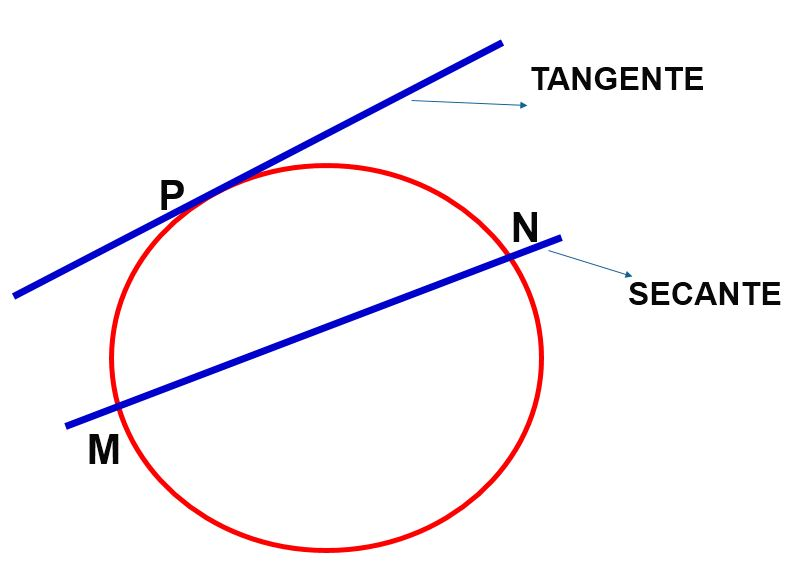
\includegraphics[width=5cm]{recta_seccante} 	\label{recta_seccante}}


	\subfigure[Recta que pasa por $ P_{1} $ y $ P_{2} $.]{
		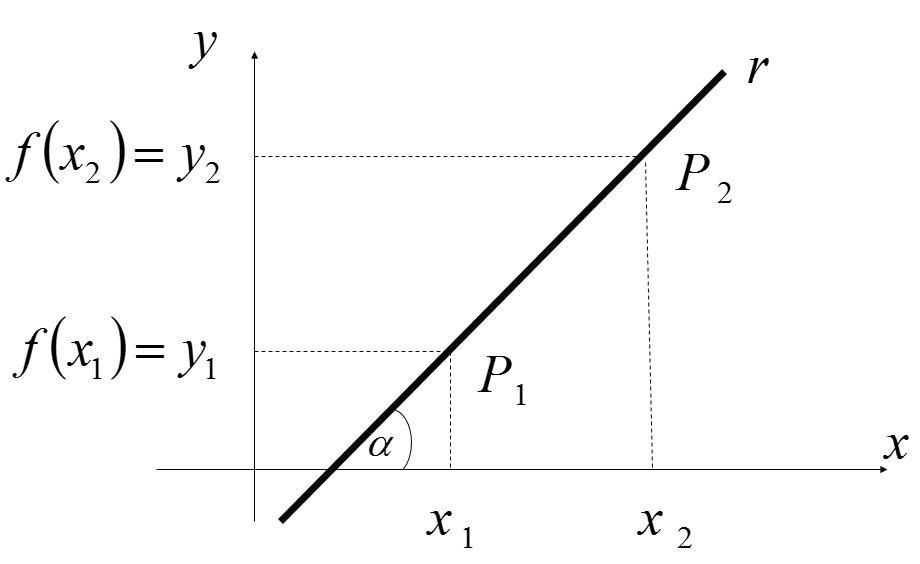
\includegraphics[width=5cm]{pendiente} \label{pendiente}}
	
		\caption{}
\end{figure}


\textsl{Recordatorio}:\\
La pendiente de una recta que pasa por dos puntos es $ m=\dfrac{y_{2}-y_{1}}{x_{2}-x_{1}} $, la ecuación de la recta es $ y=mx+n $.\\
\subsubsection{Problema matemático}

Sea una curva $ C $ dad por la ecuación $ y=f(x) $ donde la función $ f $ es continua en el intervalo $ (a,b) $. Sea $ P(x_{0},y_{0})$,  con $ x_{0}\in(a,b) $ un punto fijo de $ C $ y $ Q(x,f(x)) $ un punto variable, tal que $ x\in(a,b) $. Ver (\ref{curva_con_secante}).\\
\begin{figure}[h]
	\centering
	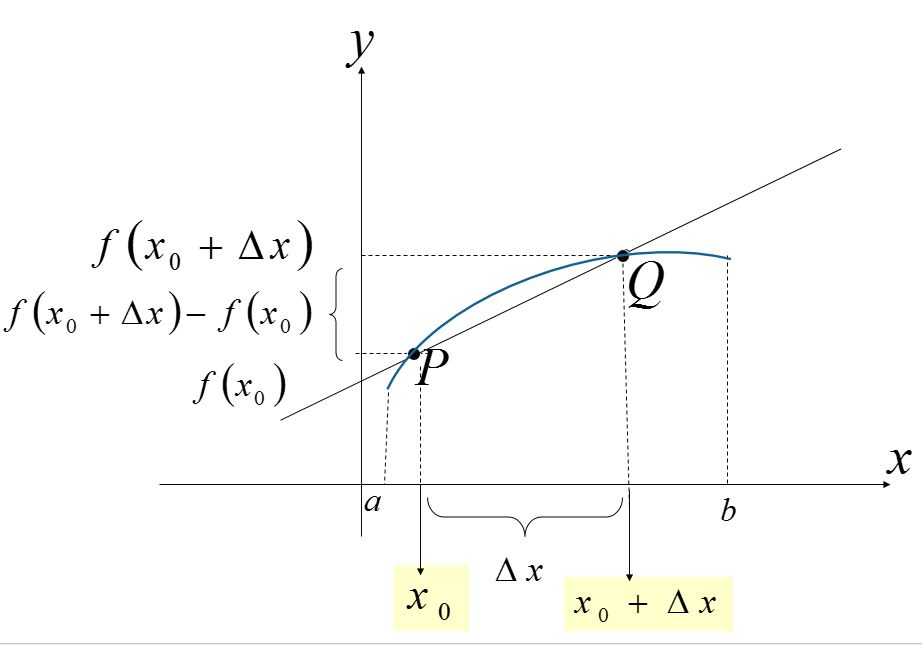
\includegraphics[width=10cm]{curva_con_secante} 
	\caption{Curva con secante}
	\label{curva_con_secante}
\end{figure}

Como se puede apreciar entre el punto $ P $ y el $ Q $, se puede trazar una recta secante a la curva, con pendiente
\[ m_{sec}=\dfrac{f(x_{0}+\Delta x)-f(x_{0})}{\Delta x} \]
Si trazamos sucesivas rectas secantes con $ x $ cada vez más cerca de $ x_{0} $. Es decir $ x\rightarrow x_{0} $ o lo que es lo mismo $ \Delta x\rightarrow0 $. Se obtendr\'a que la recta límite esuna recta tangente a la curva en el punto $ P $.

\begin{figure}[h]
	\centering
	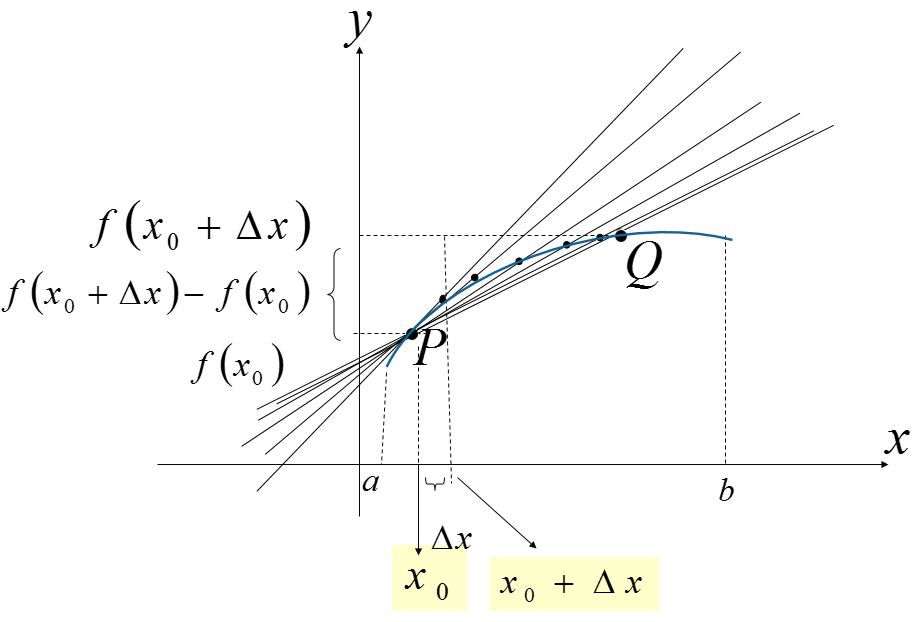
\includegraphics[width=10cm]{curvas_con_secantes}
	\label{curvas_con_secantes}
	\caption{Interpretaci\'on geom\'etrica}
\end{figure}



Por otra parte hay que tener en cuenta que la tangente es una razón trigonométrica
\begin{equation}
\tan\alpha=\dfrac{CO}{CA}=\dfrac{\Delta y}{\Delta x}=\dfrac{f(x_{0}+\Delta x)-f(x_{0})}{\Delta x}
\end{equation}










\subsubsection{Problema físico}
%%%%%%%%%%%%%%%%%%%%%%%%%%%%%%%%%%%%%%%%%%%%%%%%%%%%%%%%%%%%%%%%%%%%%%%%%%%%%%%%%%%%%%%%%%%%%%%%%%%%%%%%%%%%%%%%%%%%%%%%%%%%
Dado un cuerpo que se mueve siguiendo la ley $ s=f(t) $ tiempo en función del desplazamiento. Cuando transcurre un lapso  $ \Delta t $, ocurre un desplazamiento de tamaño $ \Delta s $
\begin{equation}
V_{media}=\dfrac{f(t_{0}+\Delta t)-f(t_{0})}{\Delta t}=\dfrac{\Delta s}{\Delta t}
\end{equation}
Una fórmula muy conocida por todos, \textsf{velocidad igual a desplazamiento sobre tiempo}, es lo que se acostumbra a decir. Pero si se fijan bien solo se cambió de contexto lo visto en el problema matemático, y esa sigue siendo la fórmula de una pendiente a una recta secante. En conclusión, la interpretación física está en que las velocidades medias van tendiendo a la velocidad instantánea.





%%%%%%%%%%%%%%%%%%%%%%%%%%%%%%%%%%%%%%%%%%%%%%%%%%%%%%%%%%%%%%

\subsection{Concepto de derivada}

%%%%%%%%%%%%%%%%%%%%%%%%%%%%%%%%%%%%%%%%%%%%%%%%%%%%%%%%%%%%%%%%%%%%%%%%%%%%%
\begin{thm}
Sea la función $ y=f(x) $ definida en cierto punto $ x_{0}\in\mathbb{R} $, y $ x $ un punto arbitrario de ese entorno. Si la relación
\[ \dfrac{f(x)-f(x_{0})}{x-x_{0}} \]
tiene límite, entonces se conoce como derivada a:
\[ f'(x_{0})=\lim\limits_{x\rightarrow x_{0}}\dfrac{f(x)-f(x_{0})}{x-x_{0}} \]
Donde:\\
$ \Delta x= x-x_{0} $ es el incremento por el eje de las $ x $.\\
$ \Delta y=f(x)-f(x_{0} $ es el incremento por el eje de las $ y $.\\

A la expresión $ y=\dfrac{\Delta y}{\Delta x} $ se le conoce también como el límite del cociente incremental.
	
\end{thm}
Son usadas para el c\'alculo límite por la definición las siguientes fórmulas:
\begin{enumerate}\label{ecuaciones_derivadas}
	\item $ f'(x_{0})=\lim\limits_{x\rightarrow x_{0}}\dfrac{f(x)-f(x_{0})}{x-x_{0}} $.
	\item $ f'(x)=\lim\limits_{\Delta x\rightarrow 0}\dfrac{f(x+\Delta x)-f(x)}{\Delta x} $.
	\item $ f'(x)=\lim\limits_{\Delta x\rightarrow 0}\dfrac{\Delta y}{\Delta x} $.
\end{enumerate}
Todas son equivalentes, su uso está en dependencia del fin de la demostración.
%%%%%%%%%%%%%%%%%%%%%%%%%%%%%%%%%%%%%%%%%%%%%%%%%%%%%%%%%%%%%%%%%%%%%%%%%%%%%%%%%%%%%%%%%%%%%%%%%%%%%%%%%%%%%%%%%%%%%%%%%%%%
\subsection{Reglas de derivaci\'on más usadas}




%\begin{equation}
%[cf(x)]'=\lim\limits_{\Delta x\rightarrow 0}\dfrac{cf(x+\Delta x)-cf(x)}{\Delta x} 
%\end{equation}
%Fueron extra\'idas de (\ref{ecuaciones_derivadas}).
%\begin{equation}
%[cf(x)]'=c\cdot\lim\limits_{\Delta x\rightarrow 0}\dfrac{f(x+\Delta x)-f(x)}{\Delta x} 
%\end{equation}
{\fboxsep 8pt\fboxrule 1pt \label{propiedades_derivadas}
Dada una funciones derivables $ f(x), g(x) $ con $ g(x)\neq0 $
\[ \fbox{$\displaystyle[cf(x)]'=cf'(x)$} \]
\[ \fbox{$\displaystyle[cf(x)]'=c\cdot f'(x)$} \]
\[ \fbox{$\displaystyle[f(x)+g(x)]'=f'(x)+g'(x)$} \]
\[ \fbox{$\displaystyle[f(x)-g(x)]'=f'(x)-g'(x)$} \]
\[ \fbox{$\displaystyle[f(x)\cdot g(x)]'=f'(x)\cdot g(x)+g'(x)\cdot f(x)$} \]
\[ \fbox{$\displaystyle\left [\frac{f(x)}{g(x)}\right ]'=\frac{f'(x)\cdot g(x)-g'(x)\cdot f(x)}{[f(x)]^{2}}$} \]
\[ \fbox{$\displaystyle(f[g(x)])'=f'[g(x)] \cdot g'(x)$} \]}
Como se ha enunciado en esta sección, estas reglas no son las únicas pero si las básicas.
%%%%%%%%%%%%%%%%%%%%%%%%%%%%%%%%%%%%%%%%%%%%%%%%%%%%%%%%%%%%%%%%%%%%%%%%%%%%%%%%%%%%%%%%%%%%%%%%%%%%%%%%%%%%%%%%%%%%%%%%%%%%%%%%%%%%%%%%%%%%%%%

\subsubsection{Teoremas acerca de las propiedades de la derivadas}
\begin{teorema}
	Sean $ f $ y $ g $ dos funciones derivables en el punto $ x_{0} $, entonces las funciones $ f+g $, $ f\cdot g $ y $ f/g $ con $ g(x_{0})\neq0 $ son derivables en $ x_{0} $ y se cumple:
	\begin{enumerate}
		\item $ (f+g)'(x_{0})=f'(x_{0})+g'(x_{0}) $;
		\item $ (f\cdot g)'(x_{0})=f'(x_{0})\cdot g(x_{0})+f(x_{0})\cdot g'(x_{0}) $;
		\item $ \left (\dfrac{f}{g}\right  )'(x_{0})=\dfrac{f'(x_{0})\cdot g(x_{0})-f(x_{0})\cdot g'(x_{0})}{g^{2}(x_{0})} $
	\end{enumerate}
\end{teorema}
Si se le presta atención al caso 1, se puede notar que en otras bibliografías sale más generalizada la propiedad. Basta tomar un $ g(x)=-h(x) $, y se esta incluyendo el caso $ (f-g)'(x_{0})$.\\
\textbf{Demostraci\'on}:\\
\begin{enumerate}
	\item 	Como las funciones $ f $ y $ g $ son derivables
	\begin{equation}
	(f+g)'(x)=\lim\limits_{\Delta x\rightarrow 0}\dfrac{(f+g)(x+\Delta x)-(f+g)(x)}{\Delta x}
	\end{equation}
	Usandos las ecuaciones de (\ref{ecuaciones_derivadas}).
	\begin{equation}
	=\lim\limits_{\Delta x\rightarrow 0}\dfrac{f(x+\Delta x)+g(x+\Delta x)-(f(x)+g(x))}{\Delta x}
	\end{equation}
	\begin{equation}
	=\lim\limits_{\Delta x\rightarrow 0}\dfrac{f(x+\Delta x)-f(x)+g(x+\Delta x)-g(x)}{\Delta x}
	\end{equation}
	\begin{equation}
	=\lim\limits_{\Delta x\rightarrow 0}\dfrac{f(x+\Delta x)-f(x)}{\Delta x}
	+\lim\limits_{\Delta x\rightarrow 0}\dfrac{g(x+\Delta x)-g(x)}{\Delta x}
	\end{equation}
	y usando las ecuaciones de (\ref{ecuaciones_derivadas}) a la inversa.
	\begin{equation}
	=f'(x)+g'(x)
	\end{equation}
	Solo con el conocimiento de las propiedades de los l\'imites.$ \blacksquare $
	%%%%%%%%%%%%%%%%%%%%%%%%%%%%%%%%%%%%%%%%%%%%%%%%%%%%%%%%%%%%%%%%%%%%%%%%%%%%%%%%%%%%%%%%%%%%%%%%%%%%%%%%%%%%%%%%%%%
	\item Con las mismas hip\'otesis
	\begin{equation}
	(f\cdot g)'(x)=\lim\limits_{\Delta x\rightarrow 0}\dfrac{(f\cdot g)(x+\Delta x)-(f\cdot g)(x)}{\Delta x}
	%=f'(x)\cdot g(x)+f(x)\cdot g'(x) 
	\end{equation}
	\begin{equation}
	=\lim\limits_{\Delta x\rightarrow 0}\dfrac{(f(x+\Delta x)\cdot g(x+\Delta x))-(f(x)\cdot g(x))}{\Delta x}
	\end{equation}
Sumando y restando por $ f(x)g(x+\Delta x) $
\begin{equation}
	=\lim\limits_{\Delta x\rightarrow 0}\dfrac{f(x+\Delta x)\cdot g(x+\Delta x)-f(x)\cdot g(x)+f(x)g(x+\Delta x)-f(x)g(x+\Delta x)}{\Delta x}
\end{equation}
Agrupando convenientemente
\begin{equation}
	=\lim\limits_{\Delta x\rightarrow 0}\dfrac{f(x+\Delta x)\cdot g(x+\Delta x)-f(x)g(x+\Delta x)+f(x)g(x+\Delta x)-f(x)\cdot g(x)}{\Delta x}
\end{equation}
\begin{equation}
=\lim\limits_{\Delta x\rightarrow 0}\dfrac{f(x+\Delta x)\cdot g(x+\Delta x)-f(x)g(x+\Delta x)}{\Delta x}
+
\lim\limits_{\Delta x\rightarrow 0}\dfrac{f(x)g(x+\Delta x)-f(x)\cdot g(x)}{\Delta x}
\end{equation}
\begin{equation}
=\lim\limits_{\Delta x\rightarrow 0}\dfrac{g(x+\Delta x)(f(x+\Delta x)-f(x))}{\Delta x}
+
\lim\limits_{\Delta x\rightarrow 0}\dfrac{f(x)(g(x+\Delta x)- g(x))}{\Delta x}
\end{equation}
\begin{equation}
=g(x)f'(x)+f(x)g'(x)	\;\;\; \blacksquare 
\end{equation}


	\item Se le agreaga a las hip\'otesis la de $ g(x)\neq0 $.
	\begin{equation}
	\left (\dfrac{f}{g}\right )'(x)=\lim\limits_{\Delta x\rightarrow 0}\dfrac{\left (\dfrac{f}{g}\right )(x+\Delta x)-\left (\dfrac{f}{g}\right )(x)}{\Delta x}
	\end{equation}
	\begin{equation}
	=\lim\limits_{\Delta x\rightarrow 0}\dfrac{\left (\dfrac{f(x+\Delta x)}{g(x+\Delta x)}\right )-\left (\dfrac{f(x)}{g(x)}\right )}{\Delta x}
	\end{equation}
	Sumando y restando por $ \dfrac{f(x+\Delta x)}{g(x)} $
	\begin{equation}
	=\lim\limits_{\Delta x\rightarrow 0}\dfrac{\left (\dfrac{f(x+\Delta x)}{g(x+\Delta x)}\right )-\left (\dfrac{f(x)}{g(x)}\right )+\dfrac{f(x+\Delta x)}{g(x)}-\dfrac{f(x+\Delta x)}{g(x)}}{\Delta x}
	\end{equation}
	\begin{equation}
		=\lim\limits_{\Delta x\rightarrow 0}\dfrac{\dfrac{f(x+\Delta x)}{g(x+\Delta x)}-\dfrac{f(x+\Delta x)}{g(x)}}{\Delta x}
+		\lim\limits_{\Delta x\rightarrow 0}\dfrac{-\dfrac{f(x)}{g(x)}+\dfrac{f(x+\Delta x)}{g(x)}}{\Delta x}
	\end{equation}
	\begin{equation}
			=\lim\limits_{\Delta x\rightarrow 0}\dfrac{\dfrac{f(x+\Delta x)g(x)-f(x+\Delta x)g(x+\Delta x)}{g(x+\Delta x)g(x)}}{\Delta x}
			+		\lim\limits_{\Delta x\rightarrow 0}\dfrac{\dfrac{-f(x)+f(x+\Delta x)}{g(x)}}{\Delta x}
	\end{equation}
	\begin{equation}
	=\lim\limits_{\Delta x\rightarrow 0}\dfrac{f(x+\Delta x)\cdot(g(x)-g(x+\Delta x))}{\Delta x\cdot g(x+\Delta x)\cdot g(x)}
	+		\lim\limits_{\Delta x\rightarrow 0}\dfrac{f(x+\Delta x)-f(x)}{\Delta x\cdot g(x)}
	\end{equation}
	\begin{equation}
		=\lim\limits_{\Delta x\rightarrow 0}\dfrac{-f(x+\Delta x)\cdot(g(x+\Delta x)-g(x))}{\Delta x\cdot g(x+\Delta x)\cdot g(x)}
		+		\lim\limits_{\Delta x\rightarrow 0}\dfrac{f(x+\Delta x)-f(x)}{\Delta x\cdot g(x)}
	\end{equation}
	\begin{equation}
			=\dfrac{-f(x)g'(x)}{ g(x)\cdot g(x)}
			+	\dfrac{f'(x)}{g(x)}
	\end{equation}
	\begin{equation}
=		\dfrac{f'(x)}{g(x)}-\dfrac{f(x)g'(x)}{ g(x)\cdot g(x)}=\dfrac{f'(x)g(x)-f(x)g'(x)}{g^{2}(x)}
	 \blacksquare 
	\end{equation}
\end{enumerate}
\begin{teorema}
	\textbf{(Derivada de la función compuesta)}\\
	Si la función $ y=f(x) $ es derivable  en el punto $ x_{0} $ y la función $ z=g(y) $ lo es en $ y_{0}=f(x_{0}) $, entonces la función $ z=(g\circ f)(x) $ es derivable en $ x_{0} $ y se cumple:
	\begin{equation}
	(g\circ f)'(x_{0})=g'(f(x_{0}))\cdot f'(x_{0}) \label{Regla_de_la_cadena}
	\end{equation}
\end{teorema}
Este teorema también es conocido como la regla de la cadena. En la práctica como más se va a utilizar (\ref{Regla_de_la_cadena}) es:
\begin{equation}
 (g\circ f)'(x_{0})=f'(x_{0})\cdot g'(f(x_{0}))  
\end{equation}
Por estética, luego de que se resuelve un ejercicio casi siempre se pone adelante la derivada de la función interna.\\
\textbf{Demostración:}\\
Usando el mismo procedimiento ya visto en las anteriores demostraciones y (\ref{ecuaciones_derivadas}):\\
\begin{equation}
(g\circ f)'(x)=\lim\limits_{\Delta x\rightarrow0}\dfrac{(g\circ f)(x+\Delta x)-(g\circ f)(x)}{\Delta x}
\end{equation}
\begin{equation}
=\lim\limits_{\Delta x\rightarrow0}\dfrac{g [f(x+\Delta x)]-g[f(x)]}{\Delta x}
\end{equation}
Como $ f(x)=y $ y $ f(x+\Delta x)=y+\Delta y $, se va a multiplicar la expresión por $ \dfrac{\Delta y}{\Delta y} $
\begin{equation}
=\lim\limits_{\Delta x\rightarrow0}\dfrac{g (y+\Delta y)-g(y)}{\Delta x}\dfrac{\Delta y}{\Delta y}
\end{equation}
Como $ f $ y $ g $ son derivables $ \Delta x\rightarrow0 $ implica que $ \Delta y\rightarrow0 $
\begin{equation}
=\lim\limits_{\Delta x\rightarrow0}\dfrac{g (y+\Delta y)-g(y)}{\Delta y}\dfrac{\Delta y}{\Delta x}
\end{equation}
\begin{equation}
=\lim\limits_{\Delta y\rightarrow0}\dfrac{g (y+\Delta y)-g(y)}{\Delta y}\cdot\lim\limits_{\Delta x\rightarrow0}\dfrac{\Delta y}{\Delta x}
\end{equation}
por las f\'ormulas de (\ref{ecuaciones_derivadas}).
\begin{equation}
=g'(y)\cdot f'(x)=g'(f(x))\cdot f'(x)\;\;\blacksquare
\end{equation}
%%%%%%%%%%%%%%%%%%%%%%%%%%%%%%%%%%%%%%%%%%%%%%%%%%%%
\begin{teorema}
	\textbf{Derivada de la funci\'on inversa}\\
	Sea $ f:(a,b)\rightarrow(c,d) $ funci\'on biyectiva y continua. Si $ f $ es derivable en $ x_{0}\in(a,b) $ y $ f'(x_{0})\neq0,  $
	entonces la funci\'on inversa $ f^{-1} $, es derivable en $ y_{0}=f(x_{0}) $ y se cumple
	\begin{equation}
	(f^{-1})'(y_{0})=\dfrac{1}{f'(x_{0})}
	\end{equation}
\end{teorema}
\textbf{Demostración:}\\
\begin{equation}
(f^{-1})'(y)=\lim\limits_{\Delta x\rightarrow0}\dfrac{f^{-1}(x+\Delta x)-f^{-1}(x)}{\Delta x}
\end{equation}
Por ser $ f^{-1} $ la funci\'on inversa de $ f $.
\[ f^{-1}(x+\Delta x)-f^{-1}(x)=\Delta y \]
\[ \Delta x= f(y+\Delta y)-f(y)\]
\begin{equation}
=\lim\limits_{\Delta x\rightarrow0}\dfrac{1}{\dfrac{f(y+\Delta y)-f(y)}{\Delta y}}
\end{equation}
La continuidad de $ f $ y $ f^{-1} $, garantiza que $ \Delta x\rightarrow0\Rightarrow\Delta y\rightarrow0 $
\begin{equation}
=\lim\limits_{\Delta x\rightarrow0}\dfrac{1}{\dfrac{f(y+\Delta y)-f(y)}{\Delta y}}
=\lim\limits_{\Delta y\rightarrow0}\dfrac{1}{\dfrac{f(y+\Delta y)-f(y)}{\Delta y}}
\end{equation}
\begin{equation}
=\dfrac{1}{f'(y)}\;\;\;\blacksquare
\end{equation}
%%%%%%%%%%%%%%%%%%%%%%%%%%%%%%%%%%%%%%%%%%%%%%%%%%%%%%%%%%%%%%%%%%%%%%%%%%%%%%%%%%%%%%%%%%%%%%%%%%%%%%%%%%%%%%%%%%%%%%%%%%%%%%%%%%%%%%%%%%%%%%%%%%%%%%%%%%%%%%%%%%%%%%%%%%%%%%%%%%%%%%%%%%%%%%%%
 %%%%%
\subsection{Tabla de las derivadas (las más usadas)}
$ (c)'=0 $\\
$ (x^{n})'=n\cdot x^{n-1} $\\
$ (\log_{a}x)=\dfrac{1}{x}\log_{a}e $ en particular $ (\ln x)'= \dfrac{1}{x} $\\
$ (a^{x})'=a^{x}\cdot\ln a $ en particular  $ (e^{x})'=e^{x} $
$ (\sen x)'=\cos x $\\
$ (\cos x)'=-\sen x $\\
$ (\tan x)'=\dfrac{1}{\cos^{2} x}=\sec^{2}x $\\
$ (\cot x)'=-\dfrac{1}{\sen^{2}x}=-\csc^{2}x $\\
$ (\arcsin x)'=\dfrac{1}{\sqrt{1-x^{2}}} $\\
$ (\arccos x)'=-\dfrac{1}{\sqrt{1-x^{2}}} $\\
$ (\arctan x)'=\dfrac{1}{1+x^{2}} $\\
$ (arccot x)'=-\dfrac{1}{1+x^{2}} $\\

%%%%%%%%%%%%%%%%%%%%%%%%%%%%%%%%%%%%%%%%%%%%%%%%%%%%%%%%%%%%%%%%%%%%%%%%%%%%%%%%%%%%%%%%%%%%%%%%%%%%%%%%%%%%%%%%%%%%%%%%%%%%%%%%%%%%%%%%%%%%%%%%%%%%%%%%%%%%%%%%%%%%%%%%%%%%%%%%%%%%%%%%%%%%%%%%%%%%%%%%%%%%%%%%%%%%%%%%%%%%%%%%%%%%%%%%%%%%%%%%%%%%%%%%%%%%%%%%%%%%%%%%%%%%%%%%%%


\subsection{Derivadas de orden superior.}
Supongamos que una funci\'on $ f:(a,b)\rightarrow\mathbb{R} $ es derivable en el intervalo $ (a,b) $, entonces su función derivada $ f' $ tiene como dominio en intervalo $ (a,b) $.
Si $ f' $ es tambi\'en derivable en $ (a,b) $, entonces la derivada de $ f' $ se denomina segunda derivada de la función $ f $ y se denota por $ f''(x) $.
\[ f''(x)=[f'(x)]' \]
\begin{thm}
	Si existe la derivada $ f^{(n-1)}(x) $ de orden $ n-1 $ $ (n>2) $ en $ (a,b) $, entonces la derivada de orden $ n $ se define por
	\begin{equation}
	f^{(n)}(x)=\dfrac{d^{n}f(x)}{dx^{n}}=[f^{(n-1)}]'(x)  \hbox{ con $x\in(a,b)  $}
	\end{equation}
\end{thm}
Por convenio muchos autores toman $ f^{0}(x)=f(x) $.\\
\begin{thm}
El conjunto de las funciones $ f:(a,b)\rightarrow\mathbb{R} $ que tienen \textsf{derivada continua de orden menor o igual a $ n $}, en dicho intervalo; ser\'a denotado por $ C^{(n)}(a,b) $. En particular, es com\'un denotar por $ C^{(0)}(a,b) $ a $ C(a,b) $, al conjunto de las funciones continuas en $ (a,b) $.
\end{thm}


%%%%%%%%%%%%%%%%%%%%%%%%%%%%%%%%%%%%%
Entonces siguiendo esta notaci\'on $ C^{(\infty)}(a,b) $ denota al conjunto de las funciones que tienen derivadas continuas de todos los \'ordenes en el intervalo $ (a,b) $.\\
\begin{ejemplo}
	La funci\'on es un caso de los que pertenecen a $ C^{n}(\mathbb{R}) $.
	\begin{equation}
	\begin{array}{llll}
	f(x)=e^{x} & f'(x)=e^{x} & .... & f^{(n)}(x)=e^{x}
	\end{array}
	\end{equation}
\end{ejemplo}


\begin{propiedad}
	Si $ f,g\in C^{(n)}(a,b) $, entnces $ (f+g) $, $ (f\cdot g)\in C^{(n)}(a,b) $ y se cumplen
	\begin{enumerate}
		\item [a)]	$ \displaystyle (f+g)^{(n)}(x)=f^{(n)}(x)+g^{(n)}(x) $
		\item [b)]	$\displaystyle  (f\cdot g)^{(n)}(x)=\sum_{k=0}^{n}{n \choose k } \left (f^{(n-k)}\cdot g^{(k)}\right )(x) $
	\end{enumerate}
	donde $ {n \choose k }=
	\frac{n!}{k!\, (n-k)!} $
\end{propiedad}
Esta última  es la Fórmula de Leibniz, que guarda relación con el binomio de Newton.\\
\fbox{Todas las funciones elemnetales son de clase $ C^{(\infty)} $ en su dominio natural de definici\'on.}



%%%%%%%%%%%%%%%%%%%%%%%%%%%%%%%%%%%%%%%%%%%%%%%%%%%%%%%%%%%%%%%%%%%%%%%%%%%%%%%%%%%%%%%%%%%%%%%%%%%%%%%%%%%%%%%%%%%%%%%%%%%%%%%%%%%%%%%%%%%%%%%%%%%%%%%%%%%%%%%%%%%%%%%%%%%%%%%%%%%%%%%%%%%%%%%%%%%%%%%%%%%%%%%%%%%%%%%%%%%%%%%%%%%%%%%%%%%%%%%%%%%%%%%%%%%%%%%%%%%%%%%%%%%%%%%%%%%%%%%%%%%%%%%%%%%%%%%%%%%%%%%%%%%%%%%%%%%%%%%%%%%%%%%%%%%%%%%%%%%%%%%%%%%%%%
\subsection{Derivada de la función implícita}

%\textbf{Ejemplo}:
\begin{ejemplo}
Encuentre la derivada con respecto a $ x $ de la función $ x^{2}+y^{2}=25 $.\\
Esta es una función escrita en forma implícita. Para calcular su derivada con respecto a $ x $ es necesario llevarla a forma explícita. Lo cual en algunos casos será un proceso complicado:
\begin{equation}
 x^{2}+y^{2}=25 
\end{equation}
\begin{equation}
 y^{2}=25-x^{2} 
\end{equation}
\begin{equation}
 y=\sqrt{25-x^{2}} 
\end{equation}
**Es importante tener en cuenta que para usar esta función en forma explícita no se debe perder de vista el hecho de que la imagen son los $ y $ mayores que cero.
\begin{equation}
 f'(x)=\left[\sqrt{25-x^{2}}\right ]'=\left[(25-x^{2})^{1/2}\right]' 
\end{equation}
Hasta aquí, se han aplicado las propiedades de la potencia. Luego con las propiedades de la derivada se resuelve el ejercicio:
\begin{equation}
 f'(x)=1/2(25-x^{2})^{-1/2}\cdot (-2x) 
\end{equation}
\begin{equation}
 f'(x)=\frac{-x}{\sqrt{25-x^{2}}} \;\;\; \blacksquare 
\end{equation}

\end{ejemplo}
 
%\textbf{Teorema:}\\
\begin{teorema}
Supongamos la variable $ y $ como función continua de $ x $ definida implícitamente por la ecuación $ F(x,y)=0 $, en una vecindad del punto $ (x_{0}, y_{0}). $ Sean 
\begin{equation}
 F(x,y), \dfrac{\partial F}{\partial x}, \dfrac{\partial F}{\partial y} 
\end{equation}
funciones continuas en algún dominio D, que contenga al punto $ (x_{0}, y_{0}) $ cuyas coordenadas satisfacen la ecuación $ F(x,y)=0 $ y además en ese punto
\begin{equation}
  \dfrac{\partial F}{\partial y}\neq0  
\end{equation}

Entonces se tendrá que en el punto $ (x_{0}, y_{0}) $ exite la derivada de la función $" y "$ respecto a la variable $ "x" $ siendo esta expresada por la fórmula:
\begin{equation}\label{funcion_implicita}
 \frac{dy}{dx}\Bigg|_{x=x_{0}}=-\dfrac{\dfrac{\partial F}{\partial x}\Bigg|_{(x_{0}, y_{0})}}{\dfrac{\partial F}{\partial y}\Bigg|_{(x_{0}, y_{0})}} 
\end{equation}
	
\end{teorema}

\textbf{Nota}: $ \partial $ es el símbolo de derivada parcial, se usa en el caso de tener una función de varias variables, en este caso $ F(x,y) $ es una función de dos variables y puede ser derivada con respecto a $ x $ o a $ y $; $ \frac{\partial F}{\partial x}(x,y) $ y $ \frac{\partial F}{\partial y}(x,y)  $ respectivamente.\\

Aplicando el teorema(\ref{funcion_implicita}):\\
\begin{equation}
 F(x,y)=x^{2}+y^{2}-25\,\,\,\,\,\,\,\,\,\,\, continua 
\end{equation}
\begin{equation}
 \frac{\partial F}{\partial y}(x,y)\neq0  
\end{equation}
es continua, y se tomar\'a $ y\neq0 $
\begin{equation}
 \dfrac{\partial F}{\partial x} \,\,\,\,\,\,\,\,\,\,\, continua 
\end{equation}
	En virtud del teorema se puede encontrar la derivada de la función $ y $ respecto a la variable $ x $. En todo punto de la región del espacio excepto $ (-5,0) $ y $ (5,0) $.\\
\begin{equation}
	 g'(x)=-\frac{2x}{2y}=-\frac{x}{y} 
\end{equation}
y del caso anterior se tiene que $ y=\sqrt{25-x^{2}} $.\\
\begin{equation}
	 g'(x)=-\frac{x}{y}=-\frac{x}{\sqrt{25-x^{2}}} 
\end{equation}
	
%	{\Large Usos de la derivación implícita:}\par
%	\\
\subsubsection{Usos de la derivación implícita}
	Determinación de la recta tangente a la superficie en un punto.\\
	Volviendo al ejemplo, para calcular la recta tangente en $ x=0 $.
	 Se tiene:
\begin{equation}
	  g'(x)=-\frac{x}{y} 
\end{equation}
\begin{equation}
	  F(x,y):x^{2}+y^{2}-25=0 
\end{equation}
	 que evaluando,
\begin{equation}
	 g'(x)=0 
\end{equation}
\begin{equation}
	  F(0,y)=y^{2}-25=0\Rightarrow y^{2}=25\Rightarrow y=\pm5 
\end{equation}
	 Pero como en la definición de la función se tomó al conjunto imagen con $ y>0 $. Se tiene que la recta tangente a la curva en el punto $ x=0 $ en $ y=5 $.
	
	



%%%%%%%%%%%%%%%%%%%%%%%%%%%%%%%%%%%%%%%%%%%%%%%%%%%%%%%%%%%%%%%%%%%%%%%%%%%%%%%%%%%%%%%%%%%%%%%%%%%%%%%%%%%%%%%%%%%%%%%%%%%%%%%%%%%%%%%%%%%%%%%%%%%%%%%%%%%%%%%%%%%%%%%%%%%%%%%%%%%%%%%%%%%%%%%%%%%%%%%%%%%%%%%%%%%%%%%%%%%%%%%%%%%%%%%%%%%%%%%%%%%%%%%%%%%%%%%%%%%%%%%%%%%%%%%%%%%%%%%%%%%%%%%%%%%%%%%%%%%%%%%%%%%%%%%%%%%%%%%%%%%%%%%%%%%%%%%%%%%%%%%%%%%%%%%%%%%%%%%%%%%%%%%%%%%%%%%%%%%%%%%%%%%%%%%%%%%%%%%%%%%%%%%%%%%%%%%%%%%%%%%%%%%%%%%%%%%%%%%%%%%%%%%%%%%%%%%%%%%%%%%%%%%%%%%%%%%%%%%%%%%%%%%%%%%%%%%%%%%%%%%%%%%%%%%%%%%%%%%%%%%%%%%%%%%%%%%%%%%%%%%%%%%%%%%%%%%%%%%%%%%%%%%%%%%%%%%%%%%%%%%%%%%%%%%%%%%%%%%%%%%%%%%%%%%%%%%%%%%%%%%%%%%%%%%%%%%%%%%%%%%%%%%%%%%%%%%%%%%%%%%%%%%%%%%%%%%%%%%%%%%%%%%%%%%%%%%%%%%%%%%%%%%%%%%%%%%%%%%%%%%%%%%%%%%%%%%%%%%%%%%%%%%%%%%%%%%%%%%%%%%%%%%%%%%%%%
\subsection{Ejercicios Resueltos}

\begin{enumerate}
	\item Calcular la derivada de las siguientes funciones aplicando las propiedades.
	\begin{enumerate}
		\item[(a)]	$ y=2x^{3}-5x^{2}+7 $
		\item[(b)]	$ y=\left(\dfrac{x+1}{\sin x}\right)\cdot\exp x $
		\item[(c)]	$ f(x)=\arctan\left (\ln\left (\dfrac{1}{x}\right )\right ) $
	\end{enumerate}
	\textbf{Respuesta1}\\
\begin{enumerate}
	\item[(Respuesta-a)]
	\[  y=2x^{3}-5x^{2}+7  \]
	\[ y'=(2x^{3}-5x^{2}+7)' \]
	Por propiedad de la derivada
	\[ y'=(2x^{3})'-(5x^{2})'+(7)' \]
	\[ y'=2(x^{3})'-5(x^{2})'+(7)' \]
	Haciendo uso de la tabla de las derivadas
	\[ y'=2\cdot3x-5\cdot2x+0 \] 
	\[ y'=6x^{2}-10x \]
	
	\item[(Respuesta-b)]
	\[ y=\left(\dfrac{x+1}{\sen x}\right)\cdot\exp x \]
	\[ y'=\left (\left(\dfrac{x+1}{\sen x}\right)\cdot\exp x\right )' \]
	Si se quiere calcular la derivada hay que percatarse de que hay un cociente, una suma y un producto de funciones.\\
	Aplicacndo la propiedad de la derivada del producto
	\[ y'=\left(\dfrac{x+1}{\sen x}\right)'\cdot\exp x+\left(\dfrac{x+1}{\sen x}\right)\cdot(\exp x)' \]
	Hay que tener en cuenta de que $ \exp x=e^{x} $
	\[ y'=\left(\dfrac{x+1}{\sen x}\right)'\cdot e^{x}+\left(\dfrac{x+1}{\sen x}\right)\cdot (e^{x})' \]
	
	\[ y'=\left[\dfrac{(x+1)'\cdot\sen x -(\sen x)'(x+1)}{(\sen x)^{2}}\right]\cdot e^{x}+\left(\dfrac{x+1}{\sen x}\right)\cdot (e^{x})'
\]
	derivando con la tabla
	
	\[ y'=\left[\dfrac{(1+0)\cdot\sen x -(\cos x)(x+1)}{\sen^{2} x}\right]\cdot e^{x}+\left(\dfrac{x+1}{\sen x}\right)\cdot e^{x}
	\]
	\[ y'=\dfrac{\sen x-x\cos x-\cos x}{\sen^{2}x}\cdot e^{x}+\dfrac{x+1}{\sen x}\cdot e^{x} \]
	Ya con la derivada calculada se realiza el trabajo algebraico:\\
	\[ y'=\left [\dfrac{\sen x-x\cos x-\cos x}{\sen^{2}x}+\dfrac{x+1}{\sen x}\right ]\cdot e^{x} \]
	
	
	
	\item[(Respuesta-c)]	
	\[  f(x)=\arctan\left (\ln\left (\dfrac{1}{x}\right )\right )  \]
	Esta es una función compuesta
	\[  f'(x)=\left[\arctan\left (\ln\left (\dfrac{1}{x}\right )\right)\right]' \]
	\[ =\arctan'\left[ \ln\left (\dfrac{1}{x}\right )\right ]\cdot\ln'\left (\dfrac{1}{x}\right )\cdot\left (\dfrac{1}{x}\right )'  \]
	Haciendo uso de la tabla:
	\[ f'(x)=\dfrac{1}{1+\ln \left (\dfrac{1}{x} \right )}\cdot\dfrac{1}{(1/x)}\cdot(x^{-1})' \]
	por propiedad de la potencia $ \dfrac{1}{x}=x^{-1} $, por tanto $ \left [\dfrac{1}{x}\right ]'=\left [x^{-1}\right ]'=-x^{-2}=-\dfrac{1}{x^{2}} $.
	
	
	\[ f'(x)=\dfrac{-x^{2}}{1+\ln \left (\dfrac{1}{x} \right )}\cdot\dfrac{1}{x^{2}} \]
	\[ f'(x)=\dfrac{-1}{x+x\ln \left (\dfrac{1}{x} \right )} \]
	
	
	
	
\end{enumerate}
	
	\item	Calcula la recta tangente a la funci\'on $ x^{2}y^{2}=(y+1)^{2}(4-y^{2}) $ que pasa por el punto $ (x,y)=(0,-2) $.

\textbf{Respuesta-2}\\

Lo primero es identificar el tipo de función con el que se está trabajando,
\[ x^{2}y^{2}=(y+1)^{2}(4-y^{2}) \]
la cual, está escrita en forma implícita, pero para tener mayor organización se va a llevar a la forma $ F(x,y)=0 $.
\[ x^{2}y^{2}-(y+1)^{2}(4-y^{2})=0 \]
¿El punto $ (x,y)=(0,-2) $ pertenece a la curva?
\[ F(0,-2)=0^{2}\cdot(-2)^{2}-(-2+1)^{2}(4-(-2)^{2})=0 \]
Esta comprobación lo dice todo.\\
Calculando sus derivadas parciales
\[ \dfrac{\partial F}{\partial x}=2xy^{2} \]
\[ \dfrac{\partial F}{\partial y}=2x^{2}y-[2(y+1)(4-y^{2})+(y+1)^{2}(-2y)] \]
Según el teorema de la función implícita, la pendiente de la recta que pasa por el punto se calcula:\\
\[ m=- \dfrac{2xy^{2}}{2x^{2}y-[2(y+1)(4-y^{2})+(y+1)^{2}(-2y)]}\Bigg|_{(0,-2)}=0\]
**\textbf{Percatarse de que}  $ 2x^{2}y-[2(y+1)(4-y^{2})+(y+1)^{2}(-2y)]\Bigg|_{(0,-2)}\neq0 $, en caso contrario no se puede aplicar el teorema.
\[ y=mx+n \]
\[ -2=0\cdot0+n \]
\[ n=-2 \]
La recta buscada es $ y=-2 $.






\end{enumerate}
%%%%%%%%%%%%%%%%%%%%%%%%%%%%%%%%%%%%%%%%%%%%%%%%%%%%%%%%%%%%%%%%%%%%%%%%%%%%%%%%%%%%%%%%%%%%%%%%%%%%%%%%%%%%%%%%%%%%%%%%%%%%%%%%%%%%%%%%%%%%%%%%%%%%%%%%%%%%%%%%%%%%%%%%%%%%%%%%%%%%%%%%%%%%%%%%%%%%%%%%%%%%%%%%%%%%%%%%%%%%%%%%%%%%%%%%%%%%%%%%%%%%%%%%%%%%%%%%%%%%%%%%%%%%%%%%%%%%%%%%%%%%%%%%%%%%%%%%%%%%%%%%%%%%%%%%%%%%%%%%%%%%%%%%%%%%%%%%%%%%%%%%%%%%%%%%%%%%%%%%%%%%%%%%%%%%%%%%%%%%%%%%%%%%%%%%%%%%%%%%%%%%%%%%%%%%%%%%%%%%%%%%%%%%%%%%%%%%%%%%%%%%%%%%%%%%%%%%%%%%%%%%%%%%%%%%%%%%%%%%%%%%%%%%%%%%%%%%
%%%%%%%%%%%%%%%%%%%%%%%%%%%%%%%%%%%%%%%%%%%%%%%%%%%%%%%%%%%%%%%%%%%%%%%%%%%%%%%%%%%%%%%%%%%%%%%%%%%%%%%%%%%%%%%%%%%%%%%%%%%%%%%%%%%%%%%%%%%%%%%%%%%%%%%%%%%%%%%%%%%%%%%%%%%%%%%%%%%%%%%%%%%%%%%%%%%%%%%%%%%%%%%%%%%%%%%%%%%%%%%%%%%%%%%%%%%%%%%%%%%%%%%%%%%%%%%%%%%%%%%%%%%%%%%%%%%%%%
\subsection{Ejercicios Propuestos}
\begin{enumerate}
	\item 	Identificar la forma en que esta expresada la funci\'on y calcular su derivada
	\begin{enumerate}
		\item[(a)]	$ \begin{cases}
		x=\dfrac{1}{t}\\
		y=\dfrac{1}{t+1}
		\end{cases} $ $ t\in \mathbb{R} $
		\item[(b)]	$ f(x)=\left (\dfrac{2x}{1-x^{2}},\dfrac{x^{2}}{1-x}\right  ) $

	\end{enumerate}


	\item 	Llevar las siguientes funciones, dadas en forma param\'etrica, a forma expl\'icita
	\begin{enumerate}
		\item[(a)]	$ \begin{cases}
			x=t^{3}+3t+1\\
			y=t^{3}-3t+1
		\end{cases} $ $ t\in \mathbb{R} $
		\item[(b)]$ \begin{cases}
			x=te^{t}\\
			y=te^{-t}
			\end{cases} $ $ t\in \mathbb{R} $
		\item[(c)]$ \begin{cases}
			x=t^{3}-3\pi\\
			y=t^{3}-6\arctan t
			\end{cases} $ $ t\in \mathbb{R} $
	\end{enumerate}
	\begin{enumerate}
		\item[2.1]	Calcular su derivada.
		\item[2.2]	Calcular las rectas tangentes a la curva en el punto $ t=0 $.
	\end{enumerate}
	\item	Sea la curva:\\
	
	$ \begin{cases}
	x=\dfrac{2t}{1-(t-1)^{3}}\\
	y=\dfrac{2t^{2}}{1-(t-1)^{3}}
	\end{cases} $
	$ t\in\mathbb{R} $\\
	Calcular su derivada en $ t=1 $.
	
	\item	La curva con ecuación $ y^{2}=x^{3}+3x^{2} $ se llama cúbica de Tscherhausen. Encuentre una ecuación de la recta tangente a esta en $ (1,-2) $. ¿En cuáles puntos tiene una tangente horizontal?
	
	\item	Calcule
	\begin{enumerate}
		\item[(a)]	$ \left [ \sin\left (\dfrac{1}{\pi-x}\right )\right ]' $
		\item[(b)]	$ \left [ \sqrt[3]{|x|}\right ]' $
		
		\item[(c)]	$ \left [ e^{\sin(\ln x)}\right ]' $
	\end{enumerate}
	
	
\end{enumerate}

%fin de seccion
\newpage
 \section{Diferencial y sus aplicaciones}
 %%%%%%%%%%%%%%%%%%%%%%%%%%%%%%%%%%%%%%%%%%%%%%%%%%%%%%%%%%%%%%%%%%%%%%%%%%%%%%%%%%%%%%%%%%%%%%%%%%%%%%%%%%%%%%%%%%%%%%%%%%%%%%%%%%%%%%
 Puede confundir un poco ver este tema separado del anterior titulado derivada y sus aplicaciones; cuando la derivada y el diferencial guardan una relación muy estrecha. Se confeccionó así porque se está cumpliendo con lo que orientan las indicaciones metodológicas del curso para técnicos de ciclo corto. Lo que tendremos es una extension del tema anterior a la cual se le agrega el concepto de diferencial que es más abarcador que el de derivada.\\
 Con este concepto se abren las puertas a nuevas herramientas muy \'utiles  en el cálculo aproximado y más.
 
 
 
 %%%%%%%%%%%%%%%%%%%%%%%%%%%%%%%%%%%%%%%%%%%%%%%%%%%%%%%%%%%%%%%%%%%%%%%%%%%%%%%%%%%%%%%%%%%%%%%%%%%%%%%%%%%%%%%%%%%%%%%%%%%%%%%%%%%%%% %%%%%%%%%%%%%%%%%%%%%%%%%%%%%%%%%%%%%%%%%%%%%%%%%%%%%%%%%%%%%%%%%%%%%%%%%%%%%%%%%%%%%%%%%%%%%%%%%%%%%%%%%%%%%%%%%%%%%%%%%%%%%%%%%%%%%% 




 \subsection{Diferencial en una variable}
  %%%%%%%%%%%%%%%%%%%%%%%%%%%%%%%%%%%%%%%%%%%%%%%%%%%%%%%%%%%%%%%%%%%%%%%%%%%%%%%%%%%%%%%%%%%%%%%%%%%%%%%%%%%%%%%%%%%%%%%%%%%%%%%%%%%%%%
  
  
  
  
  
 %%%%%%%%%%%%%%%%%%%%%%%%%%%%%%%%%%%%%%%%%%%%%%%%%%%%%%%%%%%%%%%%%%%%%%%%%%%%%%%%%%%%%%%%%%%%%%%%%%%%%%%%%%%%%%%%%%%%%%%%%%%%%%%%%%%%%%
  La relación con la noción intuitiva y geométrica de derivada,se ve con el concepto de diferencial. 
  Este viene con la necesidad de rectificar una curva.\\
\begin{figure}[h]
	\centering
	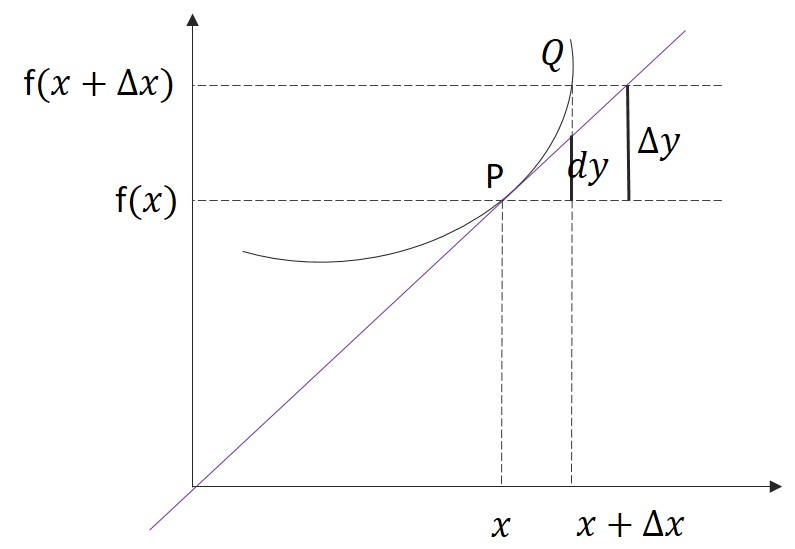
\includegraphics[width=9cm]{curva_diferencial}
	\label{curva_diferencial}
	\caption{Representación geométrica del diferencial y el incremento.}
\end{figure}
\begin{thm}
	Una función $ y=f(x) $ se llama diferenciable en el punto $ x $, si el incremento de la función puede ser representado en la forma
	\begin{equation}
	\Delta y=A\Delta x+\alpha\Delta x\label{diferencial}
	\end{equation}
	donde $ A $ es un número independiente de $ \Delta x $ y $ \alpha\rightarrow0 $ cuando $ \Delta x\rightarrow0 $.
\end{thm}  

\begin{teorema}
	Para que un función $ y=f(x) $ sea diferenciable en el punto $ x $ es necesario y suficiente que la función tenga derivada en el punto x.
\end{teorema}
\textbf{  Demostraci\'on}\\
$ (\Rightarrow) $
Supongamos que la funci\'on $ f(x) $ es diferenciable en $ x\in(a,b) $. Entonces su incremento 
\[  	\Delta y=A\Delta x+\alpha\Delta x  \]
al ser dividido por $ \Delta x\neq0 $
\begin{equation}
	\dfrac{\Delta y}{\Delta x}=\dfrac{A\Delta x+\alpha\Delta x}{\Delta x}
\end{equation}
\begin{equation}
\dfrac{\Delta y}{\Delta x}=A+\alpha
\end{equation}
pasando al límite cuando $ \Delta x\rightarrow0 $, se tiene
\begin{equation}
\lim\limits_{\Delta x\rightarrow0}\dfrac{\Delta y}{\Delta x}=A
\end{equation}
Recordar que $ A $ no dependía de $ \Delta x $ y que $ \alpha\rightarrow0 $ cuando $ \Delta x\rightarrow0 $. Esta ecuación coincide con (\ref{ecuaciones_derivadas}), por lo tanto diferenciable implica derivable.\\
$ (\Leftarrow) $\\
  Supongamos que la función es derivable en x
\begin{equation}
  \lim\limits_{\Delta x\rightarrow0}\dfrac{\Delta y}{\Delta x}=f'(x)
\end{equation}
 definici\'on de l\'imite de un funci\'on, la diferencia
 \begin{equation}
 \alpha=\dfrac{\Delta y}{\Delta x}-f'(x)
 \end{equation}  
 tiende a cero cuando $ \Delta x\rightarrow0 $.\\
 Si son multiplicados los t\'erminos de la igualdad por $ \Delta x $
 \begin{equation}
 \alpha\Delta x=\Delta y-f'(x)\Delta x
 \end{equation}
  \begin{equation}
  \Delta y=f'(x)\Delta x+\alpha\Delta x
  \end{equation}
  
  por la definici\'on de diferencial se tiene que ya llegamos a donde se quer\'ia $ \blacksquare $.\\
  \begin{center}
  \fbox{Con funciones $ f:\mathbb{R}\rightarrow\mathbb{R} $ se tiene que 
  	derivada $ \Leftrightarrow $ diferencial }
 \end{center}
  
  
  \textbf{Consideraciones}\\
  El diferencial de $ x $ variable independiente coincide con su incremento 
  \[ \Delta x=dx \]
  \[ 
  \begin{array}{ll}
  dy\approx f'(x)dx & f'(x)\approx\dfrac{dy}{dx}
  \end{array}dy \]
  El diferencial de una funci\'on difiere de la derivada solamente de un factor $ dx $. Su búsqueda se resume al c\'alculo de la derivada. Los teoremas que se refieren a las derivadas siguensiendo v\'alidos para el diferencial.\\
  \textbf{Reglas de diferenciaci\'on:}\\
  \begin{enumerate}
  	\item $ d(c\cdot f)=c\cdot df $ donde $ c=cte $.
  	\item $ d(f\mp g)=df\pm dg $
  	\item $ d(f\cdot g)=g\cdot df+f\cdot dg $
  	\item $ d\left (\dfrac{f}{g}\right )=\dfrac{gdf-fdg}{g^{2}} $; $ g\neq0 $
  	\item En el caso de la funci\'on compuesta $ y=f(g(x)) $
  	\begin{equation}
  	\dfrac{dy}{dx}=\dfrac{df}{dx}=\dfrac{df}{dg}\cdot\dfrac{dg}{dx}=f'(g(x))g'(x)
  	\end{equation}
  \end{enumerate}
  \textbf{Observaciones:}\\
  Cuando se estudian las funciones reales que dependen de dos o más variables, los
  conceptos función diferenciable y diferencial adquieren mayor complejidad. Entonces las
  nociones de función derivable y diferenciable dejan de ser equivalentes y el diferencial de
  una función en un punto se concibe como una aplicación lineal del espacio $ \mathbb{R}^{n}(n>1) $ en $ \mathbb{R} $.
  
  
  
  
  \subsubsection{C\'alculo aproximado}
   %%%%%%%%%%%%%%%%%%%%%%%%%%%%%%%%%%%%%%%%%%%%%%%%%%%%%%%%%%%%%%%%%%%%%%%%%%%%%%%%%%%%%%%%%%%%%%%%%%%%%%%%%%%%%%%%%%%%%%%%%%%%%%%%%%%%%%
  El diferencial es muy útil en el cáculo aproximado de magnitudes de forma rápida.
  \begin{equation}
  \Delta y\approx dy
  \end{equation}
  \begin{equation}
  f(x+\Delta x)-f(x)=f'(x)dx\label{resultado_util}
  \end{equation}
  Son resultados muy \'utiles para el c\'alculo aproximado.
  \begin{ejemplo}
  	Calcular aproximadamente\\
  	\[ \sqrt{\dfrac{(2.03)^{2}-3}{(2.03)^{2}+5}} \]
  	Lo primero es notar la similitud con la funci\'on 
\[ f(x)=\sqrt{\dfrac{x^{2}-3}{x^{2}+5}} \]
\begin{equation}
f'(x)=\sqrt{\dfrac{x^{2}+5}{x^{2}-3}}\cdot\dfrac{2x(x^{2}-3)-2x(x^{2}+5)}{(x^{2}+5)^{2}}
\end{equation}
Ahora se tomar\'a
\[ 
\begin{array}{lll}
x+\Delta x=2.03 & x=2 & \Delta x= 0.03
\end{array}
 \]
 Usando (\ref{resultado_util})
 \begin{equation}
 f(2.03)=f(2)+f'(2)\cdot0.03
 \end{equation}
 \begin{equation}
 =\dfrac{1}{3}+\left (\dfrac{-10}{3}\right )\cdot\dfrac{3}{100}
 \end{equation}
 \begin{equation}
 f(2.03)=0.233
 \end{equation}
  \end{ejemplo}
  
  \subsection{Teoremas Fermat, Rolle, Lagrange, Cauchy y Regla de L'Hopital}
 %%%%%%%%%%%%%%%%%%%%%%%%%%%%%%%%%%%%%%%%%%%%%%%%%%%%%%%%%%%%%%%%%%%%%%%%%%%%%%%%%%%%%%%%%%%%%%%%%%%%%%%%%%%%%%%%%%%%%%%%%%%%%%%%%%%%% %%%%%%%%%%%%%%%%%%%%%%%%%%%%%%%%%%%%%%%%%%%%%%%%%%%%%%%%%%%%%%%%%%%%%%%%%%%%%%%%%%%%%%%%%%%%%%%%%%%%%%%%%%%%%%%%%%%%%%%%%%%%%%%%%%%%% %%%%%%%%%%%%%%%%%%%%%%%%%%%%%%%%%%%%%%%%%%%%%%%%%%%%%%%%%%%%%%%%%%%%%%%%%%%%%%%%%%%%%%%%%%%%%%%%%%%%%%%%%%%%%%%%%%%%%%%%%%%%%%%%%%%%%
 En esta sección se verán n conjunto de teoremas relacionados con el comportamiento de las funciones derivables.
 \begin{figure}
 	\centering
 	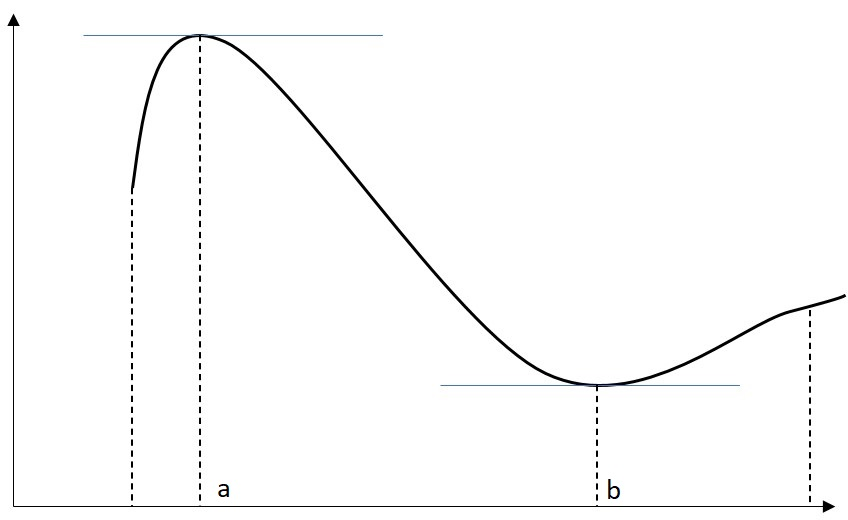
\includegraphics[width=5cm]{fermat1}
 	\caption{En el punto $ x=a $ se alcanza un m\'aximo y en el $ x=b $ un m\'inimo.}
 	\label{fermat1}
 \end{figure}
 \begin{teorema}
 	( Teorema de Fermat)
 	Sea la función definida en cieto entorno del punto $ x_{0} $ y que toma en ese punto su valor máximo o mínimo. Entonces, si para $ x=x_{0} $ existe la derivada en el punto en el sentido amplio, ella es igual a cero.(ver \ref{fermat1})
 \end{teorema}
 Este teorema nos brinda como resultado que es posible encontrar los extremos de una función con encontrar el punto donde su derivada es igual a cero.\\
 \textbf{Demostración:}\\
 Sea la funci\'on definida en el entorno $ U(x_{0}) $ del punto $ x_{0} $, suponamos que en ese punto la funci\'on alcanza un m\'aximo. 
 Como es un máximo se cumple en la vecindad que $ f(x)\leq f(x_{0}) $ para todo punto $ x\in U(x_{0}) $.
 Entonces si se hace tender por la derecha a un punto de la vecindad hasta llegar al $ x_{0} $, se observ\'a el comportamiento de las secantes, las cuales se\'an igual a 
 \begin{equation}
\dfrac{ f(x)-f(x_{0})}{x-x_{0}}\leq0
 \end{equation}
 que indica que la pendiente es negativa y por tanto en ese intervalo la funci\'on es decreciente.\\
 Repitiendo el mismo porcedimiento pero por la izquierda, se tiene
 \begin{equation}
 \dfrac{ f(x)-f(x_{0})}{x-x_{0}}\geq0
 \end{equation}
 Si existe la derivada en el punto $ x_{0} $
 \begin{equation}
 \lim\limits_{x\rightarrow x_{0}} \dfrac{ f(x)-f(x_{0})}{x-x_{0}}\geq0
 \end{equation}
\begin{equation}
 \lim\limits_{x\rightarrow x_{0}} \dfrac{ f(x)-f(x_{0})}{x-x_{0}}\leq0
\end{equation} 
 Ambas desigualdades se cumplen simult\'aneamente cuando son cero; 
 \begin{equation}
 \lim\limits_{x\rightarrow x_{0-}} \dfrac{ f(x)-f(x_{0})}{x-x_{0}}=0=\lim\limits_{x\rightarrow x_{0+}} \dfrac{ f(x)-f(x_{0})}{x-x_{0}}
 \end{equation}
 Lo cual se resume a
 \begin{equation}
 f'(x_{0})=0
 \end{equation}
 
 \begin{ejemplo}
 	Sea la funci\'on $ f(x)=|x| $, analice si en $ x=0 $ la funci\'on tiene un m\'inimo.\\
 	Para comenzar es necesario analizar si $ f(0)\geq f(x) $ para todo $ x $ en una vecindad; para ello es bueno apoyarse en una gr\'afica. Ver funci\'on m\'odulo en (\ref{funciones algebraicas1})
 \end{ejemplo} 
 
\begin{teorema}
	(Teorema de Rolle)\\
	Sea la función $ f $:
	\begin{enumerate}
		\item Continua sobre el segmento $ [a,b] $;
		\item derivable en cada punto del intervalo $ (a,b) $;
		\item tome valores iguales en los extremos del segmento, es decir, $ f(a)=f(b) $.
	\end{enumerate}
	Entonces; existe al menos un $ c\in(a,b) $, tal que $ f'(x)=0 $.(Ver figuras \ref{rolle})
\end{teorema}
 %%%%%%%%%%%%%%%%%%%%%%%%%%%%%%%%%%%%%%%%%%%%%%%%%%%%%%%%%%%%%%%%%%%%%%%%%%%%%%%%%%%%%%%%%%%%%%%%%%%%%%%%%%%%%%%%%%%%%%%%%%%%%%%%%%%%%%%%%%%%Imagenes
\begin{figure}[h]
\centering
\subfigure[Funci\'on con m\'as de un extremo]{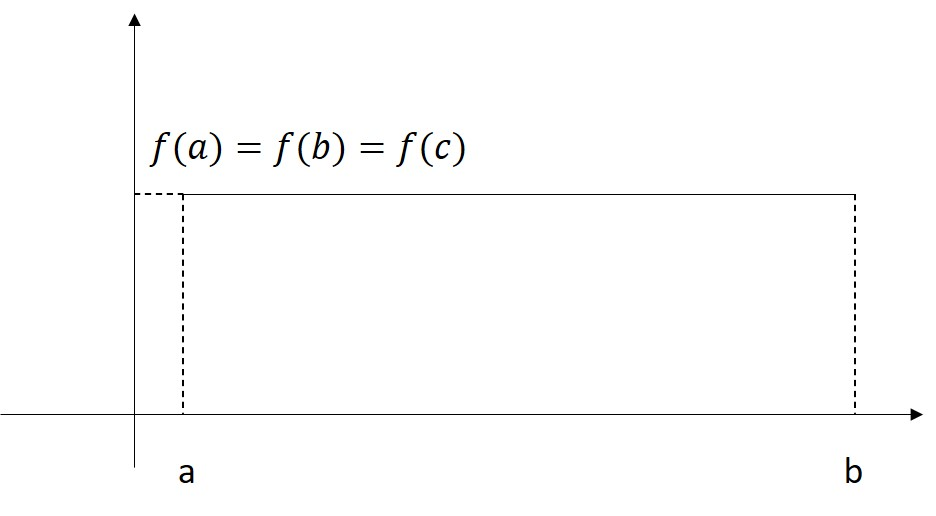
\includegraphics[width=8cm]{rolle1}}
\subfigure[Funci\'on constante]{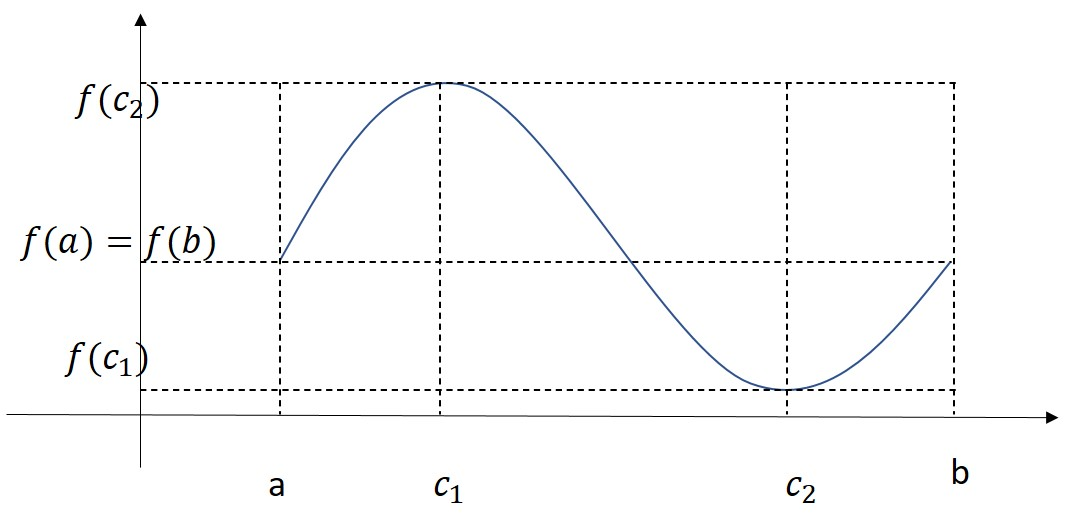
\includegraphics[width=8cm]{rolle2}}
\caption{Casos del teorema de Rolle}
\label{rolle}
\end{figure}
 \textbf{Demostración:}\\
 Por se $ f $ continua, se alcanza en ese intervalo un máximo $ M $ y un mínimo $ m $. Donde 
 \[ m=\min_{[a,b]}f(x) \]
 \[ M=\max_{[a,b]}f(x) \]
 Si $ m=M $, se tendr\'a que el máximo coincidirá con el mínimo y por lo tanto en el intervalo todos los valores serán iguales.
 \begin{equation}
 f'(c)=0
 \end{equation}
 En este caso $ c $ es cualquier valor en $ [a,b] $.\\
 Ahora si $ M\neq m $ que por su definici\'on es $ M>m $. Como una de las hipótesis del teorema me exige $ f(a)=f(b) $, como $ M\neq m $; imposible que se alcancen en los extremos del intervalo ambos valores a la vez. Por otro lado estas hipótesis obligan a que exista al menos un extremo en el intervalo. Y para ser encontrado se pueda aplicar el teorema de Fermat.$ \blacksquare $
 
 
  
 \begin{teorema}
 	(De Lagrange), también teorema del valor medio.\\
 	Si $ f $ es continua en $ [a,b] $ y derivable en $ (a,b) $; entonces existe un $ c\in(a,b) $ tal que 
 	\begin{equation}
 	f'(c)=\dfrac{f(b)-f(a)}{b-a}\label{valorMedio}
 	\end{equation}
  \end{teorema}
 Ver (figura \ref{lagrange1}).\\
 \begin{figure}[h]
 	\centering
 	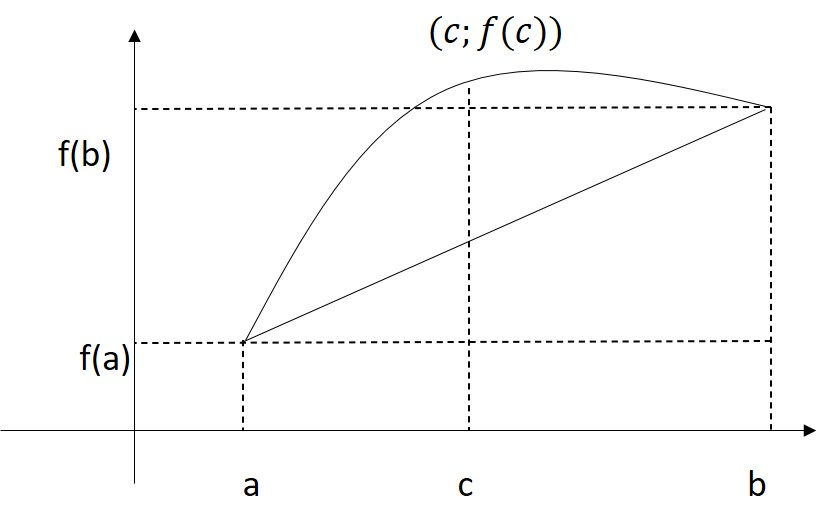
\includegraphics[width=8cm]{lagrange1}
 	\caption{Gráfica de una recta y una curva diferenciable en el intervalo $ [a,b] $.}
 	\label{lagrange1}
 \end{figure}
 \textbf{Demostración:}\\
 Teniendo en cuenta una recta que pasa por $ (a,f(a)) $ y $ (b,f(b)) $. Esta recta será llamada $ L $
 \begin{equation}
 y=\dfrac{f(b)-f(a)}{b-a}(x-a)+f(a)
 \end{equation}
 La función auxiliar formada por la diferencia entre las ordenadas de la curva $ L $ y $ f $, queda del siguiente modo
 \begin{equation}
 h(x)=f(x)-\left [ \dfrac{f(b)-f(a)}{b-a}(x-a)+f(a)\right ]
 \end{equation}
 Vemos que se cumplen  las hipótesis del teorema de Rolle
 \begin{enumerate}
 	\item $ h\in C[a,b] $, por ser la diferencia de dos funciones continuas en $ [a,b] $.
 	\item $ h\in D(a,b) $, por ser la diferencia de dos funciones derivables en $ (a,b) $.
 	\item $ h(a)=h(b) $. 
 	Como se puede ver:
 	\[ h(a)=f(a)-\left [ \dfrac{f(b)-f(a)}{b-a}(a-a)+f(a)\right ]=0 \]
 	\[ h(b)=f(b)-\left [ \dfrac{f(b)-f(a)}{b-a}(b-a)+f(a)\right ] \]
 \end{enumerate}
 Entonces por el teorema de Rolle existe $ c\in(a,b) $ tal que $ h'(c)=0 \blacksquare$.\\
 
\textbf{ *Observación}: la gráfica de $ h(x) $ es una rotación de la (\ref{lagrange1}), en la cual, la recta que intercepta a la curva, se convierte en el eje de las $ "x" $.
 \begin{corolario}
 	Sea la funci\'on $ f $
 	\begin{enumerate}
 		\item Continua sobre un intervalo finito o infinito
 		\item Con derivada nula en todos los puntos de este intervalo, a excepci\'on, opcional, de un conjunto finito.
 	\end{enumerate}
 Entonces la funci\'on es constante sobre el intervalo señalado.
 \end{corolario}
\begin{corolario}
	Si las funciones $ f $ y $ g $ son continuas sobre un intervalo y en todos sus puntos excepto en un conjunto finito de estos, tienen derivadas iguales
	\[ f'(x)=g'(x) \]
	entonces estas funciones se diferencian sobre el segmento analizado solo en una constante:
	\begin{equation}
	f(x)=g(x)+c
	\end{equation}
	$ "c" $ constante.
\end{corolario}
 \begin{ejemplo}
¿En dónde alcanza el valor medio la funci\'on $ f(x)=x^{2}+1  $ en el intervalo $ (1,3) $?
Usando el teorema del valor medio se tiene en la comprobación de hipótesis que la función es continua y derivable en el intervalo dado.
\begin{equation}
f'(x)=2x
\end{equation}
Usando la f\'ormula (\ref{valorMedio}) se tiene
\begin{equation}
f'(c)=\dfrac{f(3)-f(1)}{3-1}
\end{equation}
\begin{equation}
2c=\dfrac{10-2}{2}
\end{equation}
\begin{equation}
2c=4
\end{equation}
\begin{equation}
c=2
\end{equation}
el punto medio se alcanza en $ c=2 $.
 \end{ejemplo}
\begin{teorema}
	(Teorema de Cauchy)\\
	Sean las funciones $ f $ y $ g $
	\begin{enumerate}
		\item Continuas sobre el segmento $ [a,b] $;
		\item Tienen derivadas en cada punto del intervalo $ (a,b) $;
		\item $ g'\neq 0 $ en todos los puntos del intervalo $ (a,b) $.
	\end{enumerate}
	Entonces, existe un punto $ c\in (a,b) $, tal que
	\begin{equation}
	\dfrac{f(b)-f(a)}{g(b)-g(a)}=\dfrac{f'(c)}{g'(c)}.
	\end{equation}
\end{teorema} 
 \textbf{Demostración:}\\
 Para demostrar este teorema es útil el teorema de Rolle. Se comienza definiendo una función auxiliar
 \begin{equation}
 h(x)=f(x)-\dfrac{f(b)-f(a)}{g(b)-g(a)}\left (g(x)-g(a)\right )-f(a)
 \end{equation}
 Esta función cumple con las hipótesis del teorema de Rolle
 \begin{enumerate}
 \item $ h $	 es continua en $ [a,b] $ por ser la composición de funciones continuas.
 \item $ h $ es diferenciable en $ (a,b) $ por ser la composición de funciones difernciables.
 \item $ h(a)=h(b)=0 $
 \[  h(a)=f(a)-\dfrac{f(b)-f(a)}{g(b)-g(a)}\left (g(a)-g(a)\right )-f(a)=0 \]
 \[  h(b)=f(b)-\dfrac{f(b)-f(a)}{g(b)-g(a)}\left (g(b)-g(a)\right )-f(a)=0 \]
 \end{enumerate}
 Entonces por el teorema de Rolle, se puede encontrar un $ c\in(a,b) $ tal que $ h(c)=0 $
 \begin{equation}
  h'(x)=f'(x)-\dfrac{f(b)-f(a)}{g(b)-g(a)}g'(x)
 \end{equation}
 es la derivada.
 \begin{equation}
  h'(c)=f'(c)-\dfrac{f(b)-f(a)}{g(b)-g(a)}g'(c)
 \end{equation}
 que es igual a cero por el teroema de Rolle
 \begin{equation}
  h'(c)=f'(c)-\dfrac{f(b)-f(a)}{g(b)-g(a)}g'(c)=0
 \end{equation}
 \begin{equation}
0=f'(c)-\dfrac{f(b)-f(a)}{g(b)-g(a)}g'(c)
 \end{equation}
 \begin{equation}
\dfrac{f'(c)}{g'(c)}=\dfrac{f(b)-f(a)}{g(b)-g(a)}\blacksquare
 \end{equation}
 Este teorema también es conocido como una generalización del teorema de Lagrange. En fin, este conjunto de teoremas son uno consecuencias del otro.\\
 
 


  \subsubsection{Regla de L'Hopital}
   %%%%%%%%%%%%%%%%%%%%%%%%%%%%%%%%%%%%%%%%%%%%%%%%%%%%%%%%%%%%%%%%%%%%%%%%%%%%%%%%%%%%%%%%%%%%%%%%%%%%%%%%%%%%%%%%%%%%%%%%%%%%%%%%%%%%% %%%%%%%%%%%%%%%%%%%%%
   En algunos casos al calcular el límite de una función tenemos una indeterminación. Ver (\ref{formasIndeterminadas}), esta regla se encarga de resolver las del tipo $ \frac{\infty}{\infty} $ y   $ \frac{0}{0} $
   \begin{teorema}
   	Sea $ f,g:(a,b)\rightarrow\mathbb{R} $, diferenciables en $ (a,b) $ y supongamos que $ g(x)\neq0 \forall x\in(a,b) $. Si adem\'as
   	\begin{equation}
   	\lim_{x\rightarrow a}f(x)=\lim_{x\rightarrow a}g(x)=0
   	\end{equation}
   	O en otro caso
   	\begin{equation}
   	   	\lim_{x\rightarrow a}f(x)=\lim_{x\rightarrow a}g(x)=\infty\label{LHcaso1}
   	\end{equation}
   	Entonces 
   	\begin{equation}
   	   	\lim_{x\rightarrow a}\dfrac{f(x)}{g(x)}=\lim_{x\rightarrow a}\dfrac{f'(x)}{g'(x)}=l\label{LHcaso2}
   	\end{equation}
   	Si este l\'imite existe.
   \end{teorema}
   En la literatura suele encontrarse este teorema, m\'as conocido como regla de L'Hopital, dividido en dos teoremas. Pero en su aplicaci\'on este es el razonamiento que se tiene.\\
   \textbf{Demostración:}\\
   Para el caso de \ref{LHcaso1}, como $ f,g $ son funciones continuas en un punto $ a $ y satisfacen las condiciones de Cauchy en una vecindad de este $ a $. Se tiene que 
   \begin{equation}
   \dfrac{f(x)}{g(x)}=  \dfrac{f(x)-f(a)}{g(x)-g(a)}=  \dfrac{f'(c)}{g'(c)}
   \end{equation}
   Siendo $ c=c(x) $ un valor de $ V(a) $, vecindad de $ a $, en este caso por la derecha. Tal que $ \lim_{x\rightarrow a+}c(x)=a $.Entonces la regla del cambio de variable para l\'imites funciona y se deduce que existe
   \begin{equation}
   \lim\limits_{x\rightarrow a+}\dfrac{f'(c)}{g'(c}=k
   \end{equation}
   Luego se hace lo mismo pero con el l\'imite lateral izquierdo.
   \\
   Para probar el otro caso es similar solo hay que tener en cuenta que 
   \begin{equation}
   \dfrac{f(x)}{g(x)}=\dfrac{\dfrac{1}{g(x)}}{\dfrac{1}{f(x)}}
   \end{equation}
   $ \blacksquare $
   \begin{ejemplo}
   	Calcular\\
   	\begin{equation}
   	\lim\limits_{x\rightarrow0}\dfrac{\sen x}{x}
   	\end{equation}
   	Recordar que este el el l\'imite fundamental trigonom\'etrico y que su resultado es 1.(Ver \ref{limite_fundamental}).
   	\begin{equation}
   	\lim\limits_{x\rightarrow0}\dfrac{\sen x}{x}=\dfrac{0}{0}
   	\end{equation}
   	Esto es sabido.
   	\begin{equation}
   	\lim\limits_{x\rightarrow0}\dfrac{\sen x}{x}=\lim\limits_{x\rightarrow0}\dfrac{\cos x}{1}=1
   	\end{equation}
   	Es m\'as f\'acil, usando la regla de L'Hopital.
   \end{ejemplo}
   \begin{ejemplo}
   	Calcule\\
\[    	\lim\limits_{x\rightarrow\infty}\dfrac{\ln x}{x} \]
\begin{equation}
\lim\limits_{x\rightarrow\infty}\dfrac{\ln x}{x}=\dfrac{\infty}{\infty}
\end{equation}
Y aplicando la regla de L'Hopital se tiene
\begin{equation}
\lim\limits_{x\rightarrow\infty}\dfrac{\ln x}{x}=\lim\limits_{x\rightarrow\infty}\dfrac{1/x}{1}=\lim\limits_{x\rightarrow\infty}\dfrac{1}{x}=0
\end{equation}
   \end{ejemplo}
   
   
   
   
   
   
   
   
   %%%%%%%%%%%%%%%%%%%%%%%%%%%%%%%%%%%%%%%%%%%%%%%%%%%%%%%%%%%%%%%%%%%%%%%%%%%%%%%%%%%%%%%%%%%%%%%%%%%%%%%%%%%%%%%% 
   %%%%%%%%%%%%%%%%%%%%%%%%%%%%%%%%%%%%%%%%%%%%%%%%%%%%%%%%%%%%%%%%%%%%%%%%%%%%%%%%%%%%%%%%%%%%%%%%%%%%%%%%%%%%%%%%%%%%%%%%%%%%%%%%%%%%% %%%%%%%%%%%%%%%%%%%%%%%%%%%%%%%%%%%%%%%%%%%%%%%%%%%%%%%%%%%%%%%%%%%%%%%%%%%%%%%%%%%%%%%%%%%%%%%%%%%%%%%%%%%%%%%%%%%%%%%%%%%%%%%%%%%%%
  \subsection{B\'usqueda de extremos de funciones de una variable}
  
   %%%%%%%%%%%%%%%%%%%%%%%%%%%%%%%%%%%%%%%%%%%%%%%%%%%%%%%%%%%%%%%%%%%%%%%%%%%%%%%%%%%%%%%%%%%%%%%%%%%%%%%%%%%%%%%%%%%%%%
   
   Para la resolución de múltiples problemas de la práctica es necesaria la búsqueda de extremos. Con la localización de estos puntos se puede analizar el comportamiento de muchos procesos.\\
\begin{ejemplo}
	Sea la función $ f(x)=x^{3}+2x^{2}+3x+1 $ que modela el comportamiento del consumo energético  de un frigorífico en función de la candidad de carne que este almacena. (Caso hipotético).
\end{ejemplo}	
   Con los teoremas anteriores se puede buscar información acerca del consumo máximo, mínimo, intermedio; en función de la cantidad de carne y de cómo controlarlo.
   \begin{center}
   	¿Qué se entiende por extremo de una función?
   \end{center}
   \begin{thm}
   	Dada un función definida y continua en un segmento $ [a,b] $ es un
   	\begin{enumerate}
   		\item  máximo absoluto:
   		\[ f(x_{0})=M\geq f(x) \;\;\;\;\; \forall x\in[a,b]\]
   		\item mínimo absoluto:
   		\[ f(x_{0})=m\leq f(x) \;\;\;\;\; \forall x\in[a,b]\]
   		\item máximo relativo:
   		\[ f(x_{0})\geq f(x) \;\;\;\;\; \forall x\in V^{*}(x_{0})\]
   		\item mínimo relativo:
   		\[ f(x_{0})\leq f(x) \;\;\;\;\; \forall x\in V^{*}(x_{0})\]
   	\end{enumerate}
   	Con $ V^{*}(x_{0})={x\in \mathbb{R}| 0<|x-x_{0}|<\delta} $. Una vecindad de este intervalo.
   \end{thm}
   \fbox{Un supremo(\'infimo) es siplemente  lo mismo, lo que a diferencia del máximo(mínimo) estos no se alcanzan en el punto.}
   
   \begin{center}
\textbf{Criterio de monotonía de las funciones}
   \end{center}
   \begin{teorema}\label{Criteriomonoton}
   	Para que una función $ f $ dierenciable sobre el intervalo $ (a,b) $ crezca(decrezca) sobre ese intervalo, es necesario y suficiente que su derivada en todos los puntos de esta sea no negativa, $ f'(x)\geq0 $ (no positiva $ f'(x)\leq 0 $).
   \end{teorema}
   %%%%%%%%%%%%%%%%
    Este teorema guarda una fuerte relación con el razonamiento que hay atras del teorema de Fermat.(\ref{fermat1}) En el cual se analiza la monotonía.
   \begin{teorema}
   	(Condiciones necesarias de extremo)\\
   	Supongamos que $ x_{0} $ es un punto de extremo de la funci\'on $ f $, definida en cierto entorno del punto $ x_{0} $. Entonces o bien la derivada de $ f'(x_{0}) $ no existe, o bien $ f'(x_{0})=0 $.
   \end{teorema}
   Con este teorema se tiene una herramienta sumamente importante para la búsqueda de extremos y el análisis de los intervalos de monotonía. Pero solo es una condición necesaria y no suficiente.
   \begin{ejemplo}\label{cond}
   	Analizar si donde se anula la derivada de la función $ f(x)=x^{3}$ existe un extremo.
   	\begin{equation}
   	f'(x)=3x^{2}
   	\end{equation}
   	Es su derivada y $ f'(x)=0 $ en $ x=0 $, lo cual no es cierto. Esto se puede comprobar con el gráfico de la función.(Ver \ref{funciones algebraicas1})
   \end{ejemplo}
   Paa que este problema no nos suceda estan las condiciones suficientes.
   \begin{teorema}\label{CondicioneSuficientExtremo}
   	(Condiciones suficientes de extremo extricto)\\
   	Sea la fución $ f $ diferenciable en cierto entorno del punto $ x_{0} $, excepto, puede ser en el propio punto $ x_{0}\in(a,b)  $, en el cual es ella, sin embargo, continua. Si la derivada $ f'(x) $ cambia de signo cuando pasa por $ x_{0} $, entonces $ x_{0} $, es un punto de extremo estricto.
   \end{teorema}
   Si volvemos al ejemplo anterior (\ref{cond}) podemos comprobar que la derivada $    	f'(x)=3x^{2} $ no cambia de sigo en una vecindad de $ x_{0}=0 $; por lo tanto no se cumplen las condiciones suficientes de extremo.\\
   Ya con todo esta teor\'ia se tiene un algoritmo de trabajo para la búsqueda de extremos.
   \begin{enumerate}
   	\item Derivar la funci\'on.
   	\item Buscar los valores de $ "x" $ para los cuales se anula $ f'(x) $.
   	\item Analizar los cambios de monotonía.
   \end{enumerate}
%   \begin{ejemplo}
%   	Sea \[ f(x)=x^{3}-6x^{2}+12x+4 \]
%   	su derivada es 
%   	\begin{equation}
%   	 f(x)=3x^{2}-12x+12
%   	\end{equation}
%   	\[  f(x)=0 \]
%   	\begin{equation}
%  0=3x^{2}-12x+12
%   	\end{equation}
%   	\begin{equation}
%   	0=(x-2)^{2}
%   	\end{equation}
%   	En el punto $ x=2 $ se alcanza un posible extremo. si verificamos las condiciones suficientes de extemos
%   \end{ejemplo}
%   
    %%%%%%%%%%%%%%%%%%%%%%%%%%%%%%%%%%%%%%%%%%%%%%%%%%%%%%%%%%%%%%%%%%%%%%%%%%%%%%%%%%%%%%%%%%%%%%%%%%%%%%%%%%%%%%%%%%%%%%%%%%%%%%%%%%%%%
    \subsubsection{Criterio de la Segunda Derivada}
    Este es otro criterio que es aplicado en la clasificación de extremos. No es útil en casos donde no hay derivabilidad.
    \begin{teorema}\label{Criterio_de_la_segunda_derivada}
    	(Criterio de la segunda derivada)\\
    	Sea $ y=f(x) $ una función continua y dos veces derivable, y sea $ x=x_{0} $ un posible extremo.($ f'(x_{0})=0$). \\
    	Entonces en $ x=x_{0} $ existe un
    	\begin{enumerate}
    		\item máximo; si $ f''(x_{0})<0 $
    		\item mínimo; si $ f''(x_{0})>0 $
    		\item un punto de inflexión; si $ f''(x_{0})=0 $
    	\end{enumerate}
    \end{teorema}
\textbf{Demostración}:\\
Por la definición de derivada 
\begin{equation}
f''(x_{0})=\lim\limits_{\Delta x\rightarrow0}\dfrac{f'(x_{0}+\Delta x)-f'(x_{0})}{\Delta x}\label{segunda_derivada}
\end{equation}
ya que $ f''(x_{0})= \left[f'(x_{0})\right ]' $.\\
Como $ f'(x_{0})=0 $, la expresión (\ref{segunda_derivada}) la podemos escribir de la siguiente forma:
\begin{equation}
f''(x_{0})=\lim\limits_{\Delta x\rightarrow0}\dfrac{f'(x_{0}+\Delta x)}{\Delta x}
\end{equation}
    %
    Supongamos que $ f''(x_{0})>0 $. Entonces $ \dfrac{f'(x_{0}+\Delta x)}{\Delta x} $ debe ser positivo para $ \Delta x  $ suficientemente pequeño. Y sucede que 
    \begin{enumerate}
    	\item[o] $ f'(x_{0}+\Delta x)>0 $ con $ \Delta x>0 $
		\item[o] $ f'(x_{0}+\Delta x)<0 $ con $ \Delta x<0 $
    \end{enumerate}
    Usando el criterio de la monotonía (\ref{Criteriomonoton}) $ f $ decrece por la izquierda y crece por la derecha del punto $ x_{0} $, por lo tanto es un mínimo lo que hay en $ x_{0} $. Ver (\ref{caso1Criterio}).$ \blacksquare $\\
\begin{figure}[h]\label{casoCriterio}
	\centering
	\subfigure[La gráfica tiene un mínimo.]{
		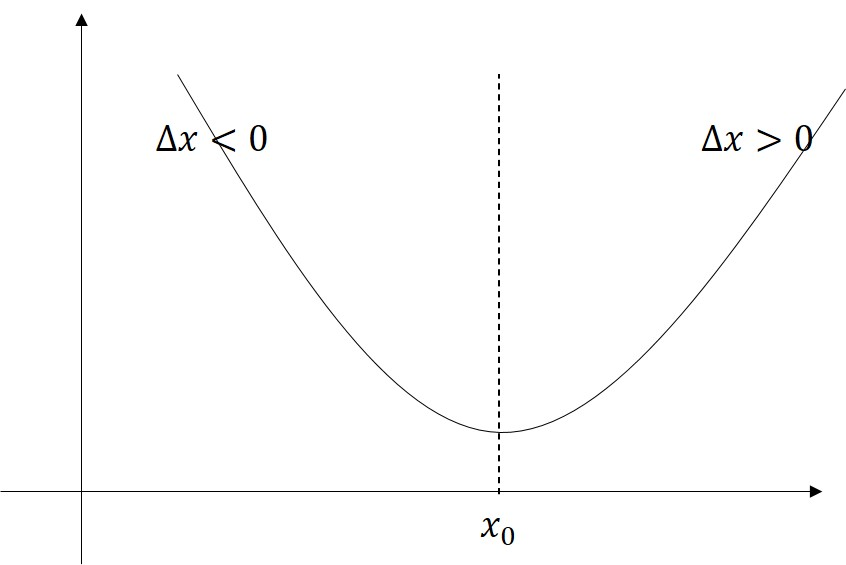
\includegraphics[width=5cm]{caso1Criterio} 	\label{caso1Criterio}}
	\subfigure[La gráfica tiene un máximo.]{
		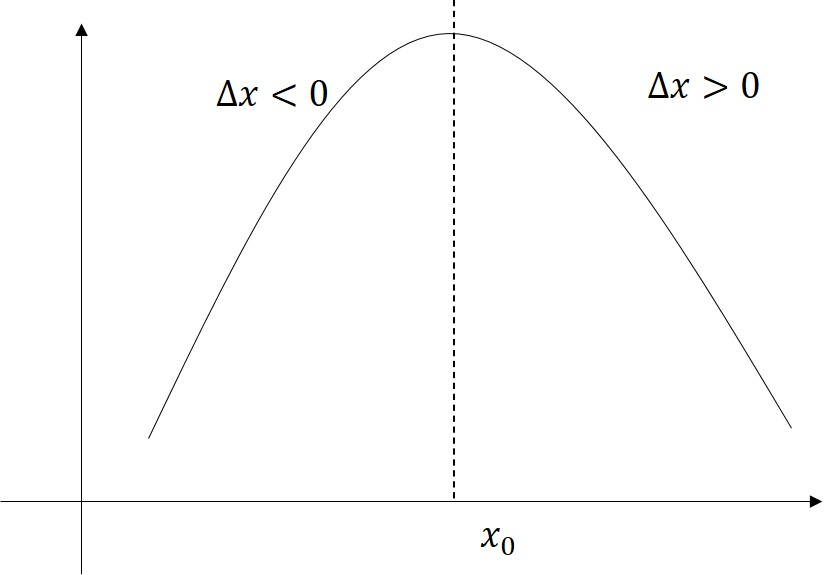
\includegraphics[width=5cm]{caso2Criterio} \label{caso2Criterio}}
	
	\caption{}
\end{figure}
Usando el mismo     razonamiento, si $ f''(x_{0})<0 $.
    sucede que 
    \begin{enumerate}
    	\item[o] $ f'(x_{0}+\Delta x)<0 $ con $ \Delta x>0 $
    	\item[o] $ f'(x_{0}+\Delta x)>0 $ con $ \Delta x<0 $
    \end{enumerate}
    $ f $ decrece por la derecha y crece por la izquierda. Ver (figura \ref{caso2Criterio})$ \blacksquare $
   \begin{ejemplo}
   	Analizar el comportamiento de la función
   	\begin{equation}
   	f(x)=x^{3}-3x+3 \;\;\;\;\;\;\;\;\;\;\;\;\;\;\;\;\mbox{en $ [-3,3/2] $}
   	\end{equation}
   	Para comoenzar con  los extremos, se calcula
   	\begin{equation}
   	f'(x)=3x^{2}-3
   	\end{equation}
   	Los posibles extremos son los puntos en los cuales se anula la derivada
   	\begin{equation}
   	f'(x)=0
   	\end{equation}
   	\begin{equation}
	0=3x^{2}-3
   	\end{equation}
   	\begin{equation}
   	x^{2}-1=0
   	\end{equation}
   	\begin{equation}
   	x^{2}=1
   	\end{equation}
   	Entonces son posibles extremos $ x=1 $ y $ x=-1 $.
   	Nos hacemos una pregunta:
   	\begin{center}
   		\textbf{¿Serán máximos, mínimos o puntos de inflexión?}
   	\end{center}
   	La respuesta esta en el criterio de la segunda derivada (\ref{Criterio_de_la_segunda_derivada})
   	\begin{equation}
   	f''(x)=6x
   	\end{equation}
   	De ahí $ 	f''(-1)=6(-1)=-6<0 $ y $ f''(1)=6(1)=6>0 $, que me da que en $ x=-1 $ hay un máximo, y en $ x=1 $, un mínimo. Y si analizamos la demostración del resultado y vemos la figura (\ref{casoCriterio}), nos podemos hacer una idea acertada de como es la gráfica de forma analítica.
   \end{ejemplo}
    Observación: en caso de que la función no tenga segunda derivada se puede usar las condiciones suficientes de extremo (\ref{CondicioneSuficientExtremo}).
    \textbf{Generalización}: (Criterio de extremos con la derivada de orden $ n $)\\
    Supongamos que $ f $ tiene en $ x_{0} $ derivadas hasta el orden $ n $ inclusive y, adem\'as
    \[ f^{(k)}(x_{0})=0,\;\;\;\;\; \mbox{$ k=1,2,...,n-1 $ y }\;\;\;\;\; f^{(n)}(x_{0})\neq0 \]
    Entonces
    \begin{enumerate}
    	\item [a)]	Si $ n $ es par, $ x_{0} $ es un punto de extremo relativo  de $ f $, mínimo cuando $ f^{(n)}(x_{0})>0 $ y máximo para $ f^{(n)}(x_{0})<0 $.
    	
    	\item [b)]	Si $ n $ es impar, $ x_{0} $ no es  extremo relativo  de $ f $. Más precisamente, cuando $ f^{(n)}(x_{0})>0 $, existe alguna vecindad donde $ V(x_{0}) $ es creciente, y cuando $ f^{(n)}(x_{0})<0 $, existe una vecindad donde $ V(x_{0}) $ es decreciente.
    \end{enumerate}
    
    
    
    
    
    
    
    
     %%%%%%%%%%%%%%%%%%%%%%%%%%%%%%%%%%%%%%%%%%%%%%%%%%%%%%%%%%%%%%%%%%%%%%%%%%%%%%%%%%%%%%%%%%%%%%%%%%%%%%%%%%%%%%%%%%%%%%%%%%%%%%%%%%%%%%
 
 \subsection{Problemas de optimizaci\'on}
  %%%%%%%%%%%%%%%%%%%%%%%%%%%%%%%%%%%%%%%%%%%%%%%%%%%%%%%%%%%%%%%%%%%%%%%%%%%%%%%%%%%%%%%%%%%%%%%%%%%%%%%%%%%%%%%%%%%%%%%%%%%%%%%%%%%%%% %%%%%%%%%%%%%%%%%%%%%%%%%%%%%%%%%%%%%%%%%%%%%%%%%%%%%%%%%%%%%%%%%%%%%%%%%%%%%%%%%%%%%%%%%%%%%%%%%%%%%%%%%%%%%%%%%%%%%%%%%%%%%%%%%%%%%% 
  Desde la antiguedad, la sociedad humana ha enfrentado situaciones como son
  usar racionalmente recursos, planificar actividades, maximizar la ganancia de la
  producción o minimizar el costo de transportar un objeto. Sin embargo, con el
  desarrollo económico, surgen problemas a gran escala y se hace necesario contar
  con un método científico que ayude a tomar decisiones para conducir y coordinar las actividades de una organizaci\'on: as\'i surge la investigaci\'on operacional.\\
  Se dice que esta aparece formalmente con el desarrollo de investigaciones conjuntas entre militares y cient\'ificos civiles para planificar operaciones de vuelo en  la Royal Air Force y posteriormente durante la Segunda Guerra Mundial. 
  Estos  problemas ya eran a gran escala, por lo que una soluci\'on em\'ipirica conllevar\'ia  grandes gastos.
   Es por esto que se precisaba de m\'etodos bien fundamentados para tomar decisiones racionales, que resuelvan la situaci\'on con ayuda de m\'aquinas
  computadoras, por ejemplo para el uso racional del radar en Gran Bretaña.
  Al estudiar un problema real, las alternativas de operación del mismo se describen, con frecuencia, a través de variables de decisión, las cuales pueden tomar
  determinados valores, mientras que el criterio de selecci\'on entre las distintas
  alternativas, se representa a partir de la minimizaci\'on de una funci\'on. Resulta
  entonces el problema:
  
  \begin{equation}
  \min f(x) s.a x\in M
  \end{equation}
  donde $ f:M\rightarrow\mathbb{R} $ y $ M\subset\mathbb{R}^{n} $ este se conoce como problema de optimización. Si además $ M $ está descrito por una cantidad finita de inecuaciones y ecuaciones,
  entonces se le llama problema de programación matemática; este término proviene de la manera en que llaman en la vida militar estadounidense a los
  proyectos.
  \begin{thm}
  	El problema de optimización en dimensión finita consiste en hallar el menor valos de la función $ f(x) $ si $ x\in M $, donde $ M\subset\mathbb{R}^{n} $. Se denota:
  	\begin{equation}
  	(P) \min f(x) \;\;\;\; s.a\;\;\;\;\; x\in M\label{ProblemaDeOptimizacion}
  	\end{equation}
  	Se lee "minimizar la funci\'on $ f $ \textbf{sujeta a} la restricci\'on $ M $"\\
  	o de la forma
  	\begin{equation}
  	(P) \min_{x\in M} f(x)
  	\end{equation}
  	 donde $ f:M\rightarrow\mathbb{R} $ y $ M\subset\mathbb{R}^{n} $.
  \end{thm}
  \begin{enumerate}
	\item   	$ x $ es el vector formado por las variables del problema o variables de decisión.
  	\item   	$ M $ denota el conjunto de soluciones factibles.

	\item   	$ f(x) $ es la función objetivo.
  	\item $ x^{*} $ resuelve $ P $ si $ x^{*}\in M $ y $ \forall x\in M $, $ f(x)\leq f(x^{*}) $. A este punto se le llama también \textsf{mínimo global de $ f $ sobre $ M $} o \textsf{solución óptima de $ P $}.
  \end{enumerate}
  El objetivo del problema (\ref{ProblemaDeOptimizacion}) es hallar los elementos del conjunto $ M $ que minimizan $ f $.
  \begin{ejemplo}
  	\[ \max x^{3}+x^{2}-2x+1 \]
  	s.a
  	\[ x\geq0 \]
  	\[ x\leq8 \]
  	tenemos como funcción objetivo a $ x^{3}+x^{2}-2x+1 $, que en este caso a diferencia  de la definición nos piden maximizar, esto es lo mismo que minimizar; solo que multiplicando por $ -1 $ a la función objetivo. El porblema esta sujeto a las restricciones:  $ x\geq0  $ y
$  x\leq8 $; que pueden ser resumidas en $ 0\leq x\leq8 $. En resumen se quiere encontrar el máximo valor de $ x $ en el intervalo $ 0\leq x\leq8 $, para ello se comenzará analizando a la función sin tener en cuenta el intervalo.
\begin{equation}
f(x)=x^{3}+x^{2}-2x+1
\end{equation}
se toma la función objetivo y se le calcula la derivada
\begin{equation}
f'(x)=3x^{2}+2x-2
\end{equation}
por la vía del discriminante se obtiene que 
\[ x_{1}=\dfrac{-1+\sqrt{7}}{3} \]
\[ x_{2}=\dfrac{-1-\sqrt{7}}{3} \]
y el caso que nos interesa es el de $ x_{1} $ que pertenece al conjunto de restricciones. $ x_{1}\approx0.55 $, que es un posible extremo. Con la segunda derivada se tiene confirmaci\'on
\begin{equation}
f''(x)=6x+2
\end{equation}
que en $ f''(0.55)=6(0.55)+2\approx5.3>0 $. Por lo tanto en el punto se alcanza un mínimo; lo que quiere decir que la función decrece hasta $ x_{1} $ y luego crece hasta el fin del conjunto de las soluciones factibles que es lo que nos atañe, todo esto por el criterio de la segunda derivada. El problema se resume a comparar entre $ x=0 $ y  $ x=8 $ cual es el que tiene mayor evaluación el la función objetivo. 
\[ 
\begin{array}{cc}
f(0)=(0)^{3}+(0)^{2}-2(0)+1 & f(8)=8^{3}+8^{2}-2\cdot8+1\\
f(0)=1                      & f(8)=561     
\end{array}
 \]
 Los números hablan por sí solos, el valor que maximiza es $ x=8 $ en el cual se alcanza el valor de $ 561 $.
  \end{ejemplo}
  
  
  
  
  
  
  
  
  
  
  
  
  
  
  
  
  %%%%%%%%%%%%%%%%%%%%%%%%%%%%%%%%%%%%%%%%%%%%%%%%%%%%%%%%%%%%%%%%%%%%%%%%%%%%%%%%%%%%%%%%%%%%%%%%%%%%%%%%%%%%%%%%%%%%%%%%%%%%%%%%%%%%%%
  
  
  
  \subsection{Ejercicios Resueltos}
  
   %%%%%%%%%%%%%%%%%%%%%%%%%%%%%%%%%%%%%%%%%%%%%%%%%%%%%%%%%%%%%%%%%%%%%%%%%%%%%%%%%%%%%%%%%%%%%%%%%%%%%%%%%%%%%%%%%%%%%%%%%%%%%%%%%%%%%%
   \begin{enumerate}%ejercicio resuelto
		\item  Puede ocurrir que la aplicación de la regla de L'Hopital no simplifique el problema. Como en este caso de 
		\begin{equation}
		\lim\limits_{x\rightarrow\infty}\dfrac{x}{\sqrt{1+x^{2}}}
		\end{equation}
   	Que a simple vista se nota que 
   	\begin{equation}
   	\lim\limits_{x\rightarrow\infty}\dfrac{x}{\sqrt{1+x^{2}}}=\dfrac{\infty}{\infty}
   	\end{equation}
   	Aplicando L'H
   	\begin{equation}
   	=\lim\limits_{x\rightarrow\infty}\dfrac{(x)'}{(\sqrt{1+x^{2}})'}=\lim\limits_{x\rightarrow\infty}\dfrac{\sqrt{1+x^{2}}}{x}
   	\end{equation}
   	Que es la función inicial invertida. Este problema se resuelve fácilmente 
\begin{equation}
   	\lim\limits_{x\rightarrow\infty}\dfrac{x}{\sqrt{1+x^{2}}}=\lim\limits_{x\rightarrow\infty}\dfrac{x}{\sqrt{x^{2}\left (1+\dfrac{1}{x^{2}}\right )}}
\end{equation}
   	\begin{equation}
   	=\lim\limits_{x\rightarrow\infty}\dfrac{x}{x\cdot\sqrt{1+\dfrac{1}{x^{2}}}}
   	\end{equation}
   	\begin{equation}
   	=\lim\limits_{x\rightarrow\infty}\dfrac{1}{\cdot\sqrt{1+\dfrac{1}{x^{2}}}}=1\blacksquare
   	\end{equation}
   	Las indeterminaciones del tipo $ 0^{0} $, $ \infty^{\infty} $ y $ 1^{\infty} $, se pueden resolver tomando previamente el logaritmo de las funciones correspondientes.\\
   	\item Calcular 
   	\begin{equation}
   	\lim\limits_{x\rightarrow0+}x^{x}
   	\end{equation}
\begin{equation}
   	=\lim\limits_{x\rightarrow0+}\ln(x^{x})
\end{equation}
   	\begin{equation}
	=\lim\limits_{x\rightarrow0+}x\ln x
   	\end{equation}
   	\begin{equation}
   		=\lim\limits_{x\rightarrow0+}\dfrac{\ln x}{1/x} 
 	\end{equation}
 	aplicando L'Hopital
 	\begin{equation}
 		=\lim\limits_{x\rightarrow0+}-\dfrac{1/x}{1/x^{2}}=	=\lim\limits_{x\rightarrow0+}-x=0
 	\end{equation}
   	Por eso en virtud de la continuidad de la función exponencial
   	\begin{equation}
   	\lim\limits_{x\rightarrow0+}x^{x}¡\lim\limits_{x\rightarrow0+}e^{x\ln x}=1\blacksquare
   	\end{equation}
   	Las indeterminaciones de las formas $ 0\cdot \infty $ y $ \infty-\infty $ se deben reducir a las formas $ 0/0 $ y $ \infty/\infty $.
   	\item Calcular\\
   	\begin{equation}
   	\lim\limits_{x\rightarrow0}\left (\dfrac{1}{x^{2}}-\cot^{2}x\right )
   	\end{equation}
   	\begin{equation}
   	=\lim\limits_{x\rightarrow0}\dfrac{\sin^{2}x-x^{2}\cos^{2}x}{x^{2}\sin^{2}x}
   	\end{equation}
   	Señalemos que 
   	\[  \dfrac{\sin^{2}x-x^{2}\cos^{2}x}{x^{2}\sin^{2}x}=\dfrac{\sin x+x\cos x}{\sin x}\cdot\dfrac{\sin x-x\cos x}{x^{2}\sin x}\]
   	El límite del primer factor de la parte derecha se halla directamente
   	\begin{equation}
   	\lim\limits_{x\rightarrow0}\dfrac{\sin x+x\cos x}{\sin x}=\lim\limits_{x\rightarrow0}\left (1+\dfrac{x}{\sin x}\cos x\right )=1
   	\end{equation}
   	Y la segunda ecuaci\'on, en la cual se aplica L'Hopital
   	\begin{equation}
   	\lim\limits_{x\rightarrow0}\dfrac{\sin x-x\cos x}{x^{2}\sin x}=\lim\limits_{x\rightarrow0}\dfrac{x\sin x}{2x\sin x+x^{2}\cos x}
   	\end{equation}
   	\begin{equation}
   	\lim\limits_{x\rightarrow0}\dfrac{1}{2+\dfrac{x}{\sin x}\cos x}=\dfrac{1}{3}
   	\end{equation}
Entonces
\begin{equation}
  	\lim\limits_{x\rightarrow0}\left (\dfrac{1}{x^{2}}-\cot^{2}x\right )=1-\dfrac{1}{3}=\dfrac{2}{3}\blacksquare
\end{equation}   	
   	
   	
   	
   \end{enumerate}%ejercicio resuelto
   
   
   
   
   
   
   
   
   
   
   
   
   
   
   
   
   
   
   
   
   
   
   
   
   
   
   
   
    %%%%%%%%%%%%%%%%%%%%%%%%%%%%%%%%%%%%%%%%%%%%%%%%%%%%%%%%%%%%%%%%%%%%%%%%%%%%%%%%%%%%%%%%%%%%%%%%%%%%%%%%%%%%%%%%%%%%%%%%%%%%%%%%%%%%%%
   \subsection{Ejercicios Propuestos}
    %%%%%%%%%%%%%%%%%%%%%%%%%%%%%%%%%%%%%%%%%%%%%%%%%%%%%%%%%%%%%%%%%%%%%%%%%%%%%%%%%%%%%%%%%%%%%%%%%%%%%%%%%%%%%%%%%%%%%%%%%%%%%%%%%%%%%%
    \begin{enumerate}%numereacion de ejercicios
    	\item Usando el diferencial calcule aproximadamente
    	\begin{enumerate}
    		\item $ \sqrt{5} $
    		\item $ \tan 46^{o} $\\
\textbf{ Sugerencia:}    		Recordar que    		$ 180grados=\pi radianes $.
    	\end{enumerate}
    	\item Un cuerpo se mueve conforme a la ley expresada por la ecuación 
    	\begin{equation}
    	s==10t+18t^{2}-2t^{3}
    	\end{equation}
    	\begin{enumerate}
    		\item ¿En el intervalo $ [1,4] $, dónde se alcanza su valor medio?
    		\item Analice su monotonía.
    	\end{enumerate}
    	
    	\item Calcule los límites
    	  \begin{enumerate}
    	  	\item $ \lim\limits_{x\rightarrow0}\dfrac{x-\sin x}{e^{x}-1-x-x^{2}/2} $
    	  	\item $ \lim\limits_{x\rightarrow0}\dfrac{\ln(1+x+x^{2})+\ln(1-x-x^{2})}{x\sin x} $
    	  	\item $ \lim\limits_{x\rightarrow0}\dfrac{(1+x)^{1/x}-e}{x} $
    	  	\item $ \lim\limits_{x\rightarrow0}\dfrac{\cos(\sin x)-\cos x}{x^{4}} $
    	  	\item $ \lim\limits_{x\rightarrow0}(\cot x)^{\sin x} $
    	  \end{enumerate}
       	\item Sean $ f(x)=x^{2}\sin \dfrac{1}{x} $ y $ g(x)=\sin x $. Halle $ \lim\limits_{x\rightarrow0}\dfrac{f(x)}{g(x)} $. Demuestre que en este caso la regla de L'Hopital no es aplicable.	
    	
    	
    	
    	
    \end{enumerate}%numereacion de ejercicios
    
    
    
    
    
    
    
    
    
    
    
    
    
    
    
    
    
    
    
    
    
    
     %%%%%%%%%%%%%%%%%%%%%%%%%%%%%%%%%%%%%%%%%%%%%%%%%%%%%%%%%%%%%%%%%%%%%%%%%%%%%%%%%%%%%%%%%%%%%%%%%%%%%%%%%%%%%%%%%%%%%%%%%%%%%%%%%%%%%% %%%%%%%%%%%%%%%%%%%%%%%%%%%%%%%%%%%%%%%%%%%%%%%%%%%%%%%%%%%%%%%%%%%%%%%%%%%%%%%%%%%%%%%%%%%%%%%%%%%%%%%%%%%%%%%%%%%%%%%%%%%%%%%%%%%%%%
 
 




\section{Integrales}
 %%%%%%%%%%%%%%%%%%%%%%%%%%%%%%%%%%%%%%%%%%%%%%%%%%%%%%%%%%%%%%%%%%%%%%%%%%%%%%%%%%%%%%%%%%%%%%%%%%%%%%%%%%%%%%%%%%%%%%%%%%%%%%%%%%%%%% %%%%%%%%%%%%%%%%%%%%%%%%%%%%%%%%%%%%%%%%%%%%%%%%%%%%%%%%%%%%%%%%%%%%%%%%%%%%%%%%%%%%%%%%%%%%%%%%%%%%%%%%%%%%%%%%%%%%%%%%%%%%%%%%%%%%%%
En el tema anterior  se estuvo resolviendo problemas relacionados con la derivada. En estos se podía realizar un cálculos aproximados, búsqueda de rectas tangentes, hallar valores medios, calcular límites, y de más. En fin, es una herramienta muy potente. ¿Pero ya que se sabe a partir de una función obtener su derivada, cómo será a la inversa?\\
La resolución de este probleba es lo que se conoce como la búsqueda de la antiderivada, o como todos dicen la integración de una función $ f $.
 
 
 
 \subsection{Integral indefinida. }
 \begin{thm}
 	Llamaremos primiteva de una función $ f(x) $ en el intervalo $ [a,b] $, a la función $ F(x) $ cuya derivada en $ [a,b] $ es igual a la función dada; esto es
 	\begin{equation}
 	F'(x)=f(x)
 	\end{equation}
 \end{thm}
 \begin{ejemplo}
 	$ F(x)=4x^{3}+2x+5 $ es primitiva de $ F'(x)=12x^{2}+2=f(x) $.\\
 	Como tambi\'en $ F(x)=4x^{3}+2x $ es primitiva de $ f $.
 \end{ejemplo}
 
% \subsubsection{Concepto de primitiva de una función}

%\begin{thm}
%	Llamaremos primitiva de una función $ f(x) $ en el intervalo $ [a,b] $ a la función $ F(x) $ cuya derivada en es igual a la función dada; es decir
%	\[ F'(x)=f(x) \]
%\end{thm}


 \begin{teorema}
 	Si en algún intervalo $ [a,b] $ la función $ F(x) $ es una primitiva para la función $ f(x) $; la función $ F(x)+c $ donde $ c $ es una constante, es también primitiva para $ f(x) $. Y viceversa, cada función que es primitiva para $ f(x) $ en $ [a,b] $ puede ser representada de la forma $ F(x)+c $.
 \end{teorema}
%  Este teorema se resume a la siguiente equivalencia:
%  \fbox{text}
   \textbf{Demostración}\\
   Como 
   \begin{equation}
   [F(x)+c]'=F'(x)+c'=f(x)
   \end{equation}
   entonces  $ F(x)+c $ es una primitiva para $ f(x) $. \\
   Ahora, con el objetivo de demostrar que todas las primitivas de una función en un intervalo dado difieren en una constante.\\
   Sea cualqier primitiva $ \varPhi(x) $ para $ f(x) $. Entonces 
   \[ \varphi'(x)=f(x) \]
   \[ F'(x)=f(x) \]
   en el intervalo $ [a,b] $. Designando 
   \begin{equation}
   \varphi(x)=\varPhi(x)-F(x)
   \end{equation}
   Derivando se tiene 
   \begin{equation}
    \varphi'(x)=[\varPhi(x)-F(x)]'= \varPhi'(x)-F'(x)=0
   \end{equation}
   para todo valor de $ x\in[a,b] $.
   Es posible en este caso aplicar el teorema de Lagrange, ya que una función derivable también es continua. En virtud de este teorema se tiene que $ \forall x\in[a,b] $
   \begin{equation}
   \varphi(x)-\varphi(a)=\varphi(c)(x-a)\;\;\;\;\;\;\;\;\;\;\;\;\; \mbox{donde $ 0<c<x $}
   \end{equation}
   Puesto que $ \varphi'(x)=0 $ se tiene que el miembro derecho de la ecuación anterior es nulo.
   \begin{equation}
   \varphi(x)-\varphi(a)=0\Leftrightarrow\varphi(x)=\varphi(a)
   \end{equation}
\textbf{   Conclusiones} 
\begin{enumerate}
\item    Las imágenes de la función $ \varphi(x) $ en el intervalo dado son iguales a $ \varphi(a) $, es decir, tenemos una función constante.
\item 	Como consecuencia de lo anterior, $ \varPhi(x)-F(x)=   c $, con $ c $ constante.
   
   
   
   
   
\end{enumerate}   
$ \blacksquare $\\

Como ocurre que si una función tiene primitiva, entonces dos primitivas de una misma función en un intervalo difieren en una constante.

\begin{thm}
	El conjunto de todas las primitivas de una función $ f $ en un intervalo dado se llama integral indefinida y se designa por $ \int f(x)dx $.
\end{thm}
   Haciendo uso del conocimiento anterior, si $ F $ es primitiva de $ f $.
   \[ \int f(x)dx=F(x)+c \]
   $ f(x) $ es conocida como la función integrando\\
   $ f(x)dx $ como la expresión integrando\\
   $ dx $ el famoso diferencial de $ x $\\
   $ \int $ el símbolo de integral indefinida.\\
   
   
   
   \subsubsection{Integrales de tabla}
   
Esta tabla se obtiene directamente de la de las derivadas (\ref{propiedades_derivadas})   
\begin{enumerate}\label{tabla_integrales}
	\item $ \displaystyle\int x^{a}dx=\dfrac{x^{a+1}}{a+1}+c $.
	\item $ \displaystyle\int \dfrac{dx}{x}=\ln |x|+c $ siempre que $ x\neq0 $.
	\item $ \displaystyle\int a^{x}dx=\dfrac{a^{x}}{\ln a}+c $, con $ a>0 $ y $ a\neq1 $, de ah\'i que $ \int e^{x}dx=e^{x}+c. $.
	\item $ \displaystyle\int \sin xdx=-\cos x+ c $.
	\item $ \displaystyle\int \cos xdx=\sin x+c $.
	\item $ \displaystyle\int\dfrac{dx}{\cos^{2}x}=\tan x+c $.
	\item $ \displaystyle\int \dfrac{dx}{\sin^{2}x}=-\cot x+c $.
	\item $ \displaystyle\int \sinh xdx=\cosh x+c $.
	\item $ \displaystyle\int \cosh xdx=\sinh x+c $.
	\item $ \displaystyle\int\dfrac{dx}{\cosh^{2} x}=\tanh x+c $.
	\item $ \displaystyle\int\dfrac{dx}{\sinh^{2} x}=-\coth x+c $.
	\item $ \displaystyle\int \dfrac{dx}{x^{2}+a^{2}}=\dfrac{1}{a}\arctan\dfrac{x}{a}+c=-\dfrac{1}{a}arccot\dfrac{x}{a}+c $.
	\item $ \displaystyle\int \dfrac{dx}{x^{2}-a^{2}}=\dfrac{1}{2a}\ln\left |\dfrac{x-a}{x+a}\right |+c $
	\item $ \displaystyle\int \dfrac{dx}{\sqrt{x^{2}-a^{2}}}=\arcsin \dfrac{x}{a}+c=-\arccos\dfrac{x}{a}+c$, con $ |x|<|a| $.
	\item $ \displaystyle\int \dfrac{dx}{\sqrt{x^{2}\pm a^{2}}}=\ln |x+\sqrt{x^{2}\pm a^{2}}|+c $, con $ |x|<|a| $.
	
	
	
	
	
\end{enumerate}
   
   
   
   
   
   
   
\subsubsection{Reglas de integración (Propiedades)}   
%%%%%%%%%%%%%%%%%%%%%%%%%%%%%%%%%%%%%%%%%%%%%%%%%%%%%%%%%%%%%%%%%%%%%%%%%%%%%%%%%%%%%%%%%%%%%%%%%%%%%%%%%%%%%%%%%%%%%%%%%%%%%%%%%%%%%%
Las reglas de integración al igual que las de derivación, nos facilitarán la resolución de problemas. De la definición de integral indefinida se deducen las mismas.
\begin{enumerate}\label{Reglas_integracion}
	\item $ \displaystyle\left [ \int f(x)dx\right ]'=f(x) $
	\item $ \displaystyle\int f'(x)dx=f(x)+c $
	\item $ \displaystyle\int \left [f(x)\pm g(x)\right]dx=\int f(x)dx\pm\int g(x)dx $
	\item $ \displaystyle\int\alpha f(x)dx=\alpha\int f(x)dx $ siendo $ \alpha $ una constante.
\end{enumerate}
Ver la similitud con las propiedades de las derivadas (\ref{propiedades_derivadas}).
 Estas se extienden igual para el diferencial, como se puede ver en 
 \begin{equation}
 \displaystyle d\left [\int f(x)dx\right ]=f(x)dx
 \end{equation}
 \begin{equation}
 \displaystyle df(x)=f(x)+c
 \end{equation}
\begin{ejemplo}
	Calcular
	\[  \displaystyle\int\left (5\cos x+2-3x^{2}+\dfrac{1}{x}-\dfrac{4}{x^{2}+1}\right )dx \]
	Primero que todo hay que aplicar las propiedades de las integrales
	\begin{equation}
	=\displaystyle\int5\cos xdx+\int2dx-\int3x^{2}dx+\int\dfrac{1}{x}dx-\int\dfrac{4}{x^{2}+1}dx
	\end{equation}
	\begin{equation}
	=\displaystyle5\int\cos xdx+2\int dx-3\int x^{2}dx+\int\dfrac{dx}{x}-4\int\dfrac{dx}{x^{2}+1}
	\end{equation}
	Ahora se busca en la tabla de las integrales
\begin{equation}
	=\displaystyle5(\sin x)+2(x)-3\left (\dfrac{x^{3}}{3}\right )+\ln |x|-4\arctan x+ c
\end{equation}
\begin{equation}
=\displaystyle5\sin x+2x-x^{3}+\ln |x|-4\arctan x+ c\blacksquare
\end{equation}
\end{ejemplo} 
\subsection{Métodos de integración}
%%%%%%%%%%%%%%%%%%%%%%%%%%%%%%%%%%%%%%%%%%%%%%%%%%%%%%%%%%%%%%%%%%%%%%%%%%%%%%%%%%%%%%%%%%%%%%%%%%%%%%%%%%%%%%%%%%%%%%%%%%%%%%%%%%%%%%%%%%%%%%%%
No todas las integrales a las que nos enfrentamos son integrales de tabla. Algunas requieren de otros procedimientos un poco más complejos para ser resueltas.





 %%%%%%%%%%%%%%%%%%%%%%%%%%%%%%%%%%%%%%%%%%%%%%%%%%%%%%%%%%%%%%%%%%%%%%%%%%%%%%%%%%%%%%%%%%%%%%%%%%%%%%%%%%%%%%%%%%%%%%%%%%%%%%%%%%%%%%%%%%%%%%%%%%%%%%%%%%%%%%%%%%%%%%%%%%%%%%%%%%%%%%%%%%%%%%%%%%%%%%%%%%%%%%%%%%%%%%%%%%%%%%%%%%%%%%%%%%%%%%%%%%%%%%%%%%%%%%%%%%%%%%%%%%%%%%%%%%
 \subsubsection{Integración por cambio de variables}
 %%%%%%%%%%%%%%%%%%%%%%%%%%%%%%%%%%%%%%%%%%%%%%%%%%%%%%%%%%%%%%%%%%%%%%%%%%%%%%%%%%%%%%%%%%%%%%%%%%%%%%%%%%%%%%%%%%%%%%%%%%%%%%%%%%%%%%
 Si observamos funciones como $ \sin 2x $ podemos notar que en la tabla de las integrales no est\'a. Estamos en presencia de una función compuesta, de la cual no tenemos reglas de integración hasta el momento. Pero con una combinación de propiedades de la derivada y la integral se puede llegar a un importante resultado. Ver (\ref{propiedades_derivadas}) y (\ref{Reglas_integracion}).\\
 Si la función $ \varphi $ es continua sobre el intervalo $ [a,b] $, es diferenciable en todos sus puntos a excepción de cierto conjunto finito y la preimagen total $ \varphi^{-1}(E_{f}) $ de conjunto $ E_{f} $ también es un conjunto finito, entonces la función $ f[\varphi (t)]\varphi'(t) $ tiene la primitiva $ F(\varphi(t)) $ sobre el intervalo $ [a,b] $.\\
 ¿Para qué nos sirve este análisis?
 Como se han podido percatar de las propiedades de la derivada se tiene que la derivada de  la función compuesta es 
 \[ \displaystyle(f[g(x)])'=f'[g(x)] \cdot g'(x) \]
 Si integramos ambos miembros se obtiene
 \begin{equation}
 \displaystyle\int(f[g(x)])'dx=\int f'[g(x)] \cdot g'(x)dx
 \end{equation}
 y haciendo a $ f=F $( como convenio se está asumiendo que $ F $ es primitiva de $ f $), a $ g=\varphi $ y a l$ f'=f $ se tiene
 \begin{equation}
 \displaystyle F[g(x)]+c=\int f[\varphi(x)] \cdot \varphi'(x)dx
 \end{equation}
 Con esto se acaba de demostrar el siguiente teorema.
 \begin{teorema}
 	Sean las funciones $ y=f(x) $ y $ x=\varphi(t) $ definidas en ciertos intervalos para que exista la función
 	compuesta $ f(\varphi(t)) $, siendo la función  $ \varphi(t) $ diferenciable. Si la función $ f(x) $ tiene primitiva, entonces la función $ f(\varphi(t))\varphi'(t) $ tiene como primitva a la funci\'on $ F[\varphi(t)] $
 	\begin{equation}
 	\displaystyle\int f(\varphi(t))\varphi'(t)dt=F[\varphi(t)]+c
 	\end{equation}
 \end{teorema}
 Entonces siguiendo este resultado el ejercicio anterior queda de la siguiente forma:
 \begin{equation}
 \int\sin2xdx
 \end{equation}
 en este caso $ \varphi=2x $ y $ d\varphi=2dx $
 \begin{equation}
 =\int \dfrac{\sin\varphi}{2} d\varphi
 \end{equation}
 Buscamos en la tabla (\ref{tabla_integrales})
 \begin{equation}
 =-\dfrac{\cos\varphi}{2}+c
 \end{equation}
 \begin{equation}
 =-\dfrac{\cos 2x}{2}+c\blacksquare
 \end{equation}
 \textbf{Procedimiento}
 \begin{enumerate}
 	\item Leer la integral e identificar si la funci\'on integrando es compuesta.(Buscar algo como $ f(g(x))) $
 	\item Calcular el diferencial de $ g(x) $, e igualarlo a $ d\varphi=g'(x)dx $, para luego con transformaciones algebraicas dejar solo en un miembro a $ dx $.
 	\item Realizar el cambio de variables.
 	\item Integral usando las propiedades y la tabla.
 	\item Realizar el cambio de variables en sentido invverso.
 \end{enumerate}
 
 \begin{ejemplo}
 	Calcular
 	\begin{equation}
 	\int \dfrac{dx}{\sqrt{a^{2}-x^{2}}}
 	\end{equation}
 	Antes hay que hacer una pequeña transformación
 	\begin{equation}
\displaystyle\int \dfrac{dx}{\sqrt{a^{2}\left (1-\dfrac{x^{2}}{a^{2}}\right )}}
 	\end{equation}
 	\begin{equation}
 	\displaystyle\dfrac{1}{a}\int \dfrac{dx}{\sqrt{1-(\dfrac{x}{a})^{2}}}
 	\end{equation}
 	Para poder identificar la función interna es de mucha utilidad un previo conocimiento de (\ref{tabla_integrales})
	 \[ \displaystyle\int \dfrac{dx}{\sqrt{x^{2}-a^{2}}}=\arcsin \dfrac{x}{a}+c=-\arccos\dfrac{x}{a}+c, \mbox{con $ |x|<|a| $.} \]
	 Entonces en nuestro caso $ t=\dfrac{x}{a} $ y $ dt=\dfrac{dx}{a} $ lo que implica que $ dx=adt $
	 \begin{equation}
	 \int \dfrac{dt}{1-t^{2}}
	 \end{equation}
es lo que se obtiene del cambio de variable.
\begin{equation}
=\arcsin t +c
\end{equation}
\begin{equation}
=\arcsin \dfrac{x}{a}+c\blacksquare
\end{equation}

 \end{ejemplo}
 
 
 
 
 
 
 
 
 
 
 
 %%%%%%%%%%%%%%%%%%%%%%%%%%%%%%%%%%%%%%%%%%%%%%%%%%%%%%%%%%%%%%%%%%%%%%%%%%%%%%%%%%%%%%%%%%%%%%%%%%%%%%%%%%%%%%%%%%%%%%%%%%%%%%%%%%%%%%
 \subsubsection{Integración por partes}
 %%%%%%%%%%%%%%%%%%%%%%%%%%%%%%%%%%%%%%%%%%%%%%%%%%%%%%%%%%%%%%%%%%%%%%%%%%%%%%%%%%%%%%%%%%%%%%%%%%%%%%%%%%%%%%%%%%%%%%%%%%%%%%%%%%%%%%%%%%%%%%%%%%%%%%%%%%%%%%
 Otra de las formas existentes para reducir una integral dada en una inmediata es mediante el método de integración por partes. El cual tiene la característica de ser útil en la integración del producto de funciones.
 \begin{ejemplo}
 	Son unos casos:
 	\begin{enumerate}
 		\item $ \displaystyle\int\ln xdx $, en este caso la función integrando esta multiplicada por una función constante que es $ f(x)=1 $.
 		\item $ \displaystyle\int x\sin xdx $, es evitente, por un lado $ "x" $ y por el otro $ \sin x $.
 		\item $ \displaystyle\int \dfrac{x}{e^{x}}dx $, $ x $ y $ \dfrac{1}{e^{x}} $.
 	\end{enumerate}
  \end{ejemplo}
  Igual que el método anterior  este se deduce de las propiedades de la derivadas.(\ref{propiedades_derivadas}).
  \begin{teorema}
  	(Fórmula de integración por partes)\\
  	Si las funciones $ u $ y $ v $ son continuamente derivables en cierto intervalo, entonces se cumple que:
  	\begin{equation}
  	\int udv=uv-\int vdu\label{integracion_por_partes}
  	\end{equation}
  \end{teorema}
 Muchos estudiantes y profesores han utilizado el recurso memotécnico de hacer referencia al miembro derecho de la expresión (\ref{integracion_por_partes}) con la frase \textsl{"\textbf{u}na \textbf{v}aca menos(-) \textbf{f}laca \textbf{v}estida \textbf{d}e \textbf{u}niforme"}.
 \textbf{Demostración:}\\
 Tenemos el producto de dos funciones diferenciables $ u $ y $ v $, de las cuales por las propiedades de las derivadas se tiene que
 \begin{equation}
 [u(x)v(x)]'=u'(x)v(x)+v'(x)u(x)
 \end{equation}
 Con tranformaciones algebraicas se tiene
 \begin{equation}
 v'(x)u(x)= [u(x)v(x)]'-u'(x)v(x)
 \end{equation}
 Integrando ambos miembros
\begin{equation}
\int v'(x)u(x)dx= \int \left ([u(x)v(x)]'-u'(x)v(x)\right )dx
\end{equation}
 Aplicando propiedades de la integral
 \begin{equation}
 \int v'(x)u(x)dx= \int[u(x)v(x)]'dx-\int u'(x)v(x)dx
 \end{equation}
 \begin{equation}
 \int v'(x)u(x)dx= u(x)v(x)-\int u'(x)v(x)dx
 \end{equation}
Calculando los diferenciales notamos que $ dv=v'(x)dx $ y que $ du=u'(x)dx $, sustituyendo en la expresión
\begin{equation}
 \int udv= uv-\int vdu\blacksquare
\end{equation}
 \begin{ejemplo}
 	Calcular $ \int \ln x dx $
\[  	\begin{array}{ll}
 		 u=\ln x  &  dv=dx \\
 		 du=\dfrac{dx}{x}  &  v=x 
 	\end{array}
 \] 
 \begin{equation}
= x\ln x-\int x\cdot\dfrac{1}{x}dx
 \end{equation}
 \begin{equation}
 =x\ln x-\int dx
 \end{equation}
 \begin{equation}
= x\ln x-x+c\blacksquare
 \end{equation}
 
 
 
 
 \end{ejemplo}
 \textbf{Procedimiento:}\\
 \begin{enumerate}
 	\item Identificar en la funci\'on integrando $ u $ y $ du $.
 	\item Hallar $ du $ y $ v $.
 	\item Hacer uso de la fórmula de integración por partes $  \int udv= uv-\int vdu $.
 	\item Aplicar propiedades de la integral hasta obtener integrales de tabla.
 	\item Calcular la integral.
 \end{enumerate}
 
 \begin{ejemplo}
 	Calcular $ \int xe^{x}dx $.
 	\begin{equation}
 	\int xe^{x}dx
 	\end{equation}
 	\[ 
 	\begin{array}{ll}
 	u=x & dv=e^{x}\\
 	du=dx & v=e^{x}
 	\end{array}
 	\]
 	\begin{equation}
 	=xe^{x}-\int e^{x}dx
 	\end{equation}
 	\begin{equation}
 	=xe^{x}-e^{x}+c=(x-1)e^{x}+c
 	\end{equation}
 \end{ejemplo}
 
 
 
 
 
 
 
 
 
 
 
 
 
 
 
 
 
 
 
 
 
 
 
\subsubsection{Integración por fracciones simples}
%%%%%%%%%%%%%%%%%%%%%%%%%%%%%%%%%%%%%%%%%%%%%%%%%%%%%%%%%%%%%%%%%%%%%%%%%%%%%%%%%%%%%%%%%%%%%%%%%%%%%%%%%%%%%%%%%%%%%%%%%%%%%%%%%%%%%%%%%%%%%%%%%%%%%%%%%%%%%%%%%%%%%%%%%%%%%%%%%%%%%%%%%%%%%%%%%%%%%%%%
 Existen otras integrales de funciones racionales que no se pueden calcular por nincçguno de los métodos estudiados que aparecen con gran frecuencia. Estas son las integrales de fracciones recionales
 \[ f(x)=\dfrac{P(x)}{Q(x)} \]
 Donde $ P(x) $ y $ Q(x) $ son polinomios.
 \begin{ejemplo}
 	\[ \int\dfrac{2x-3}{x^{2}+4x+5}dx \]
 \end{ejemplo}
 Si nos fijamos bien en el ejemplo estamos en presencia de una función integrando que es una fracción racional.
 \begin{thm}
 	Consideremos una función racional $ P/Q $ donde
 	\[ P(x)=a_{n}x^{n}+a_{n-1}x^{n-1}+...+a_{0} \]
 	\[ Q(x)=b_{m}x^{m}+b_{m-1}x^{m-1}+...+b_{0} \]
 	(Sacado de "Calculus tomo I y II -Spivak)
 \end{thm}
 En la mayoría de los casos se toman $ a_{n}=b_{m}=1 $ y  a $ n<m $, o de otro modo ser\'ia un polinomio, una parte considerable de la expresi\'on.
 \begin{ejemplo}
 	\[ \dfrac{u^{2}}{u-1}=u+1+\dfrac{1}{u-1} \]
 \end{ejemplo}
 La integración racional se basa en dos hechos; el primero de ellos es consecuencia del \textbf{Teorema Fundamental del Álgebra}
 y el segundo es la descomposición en factores de un polinomio.
 \\
 Una fracción racional puede ser descompuesta en varias fracciones simples de la forma:
 \begin{enumerate}
 	\item $  \displaystyle\int \dfrac{A}{x-a}dx  $
 	\item  $ \displaystyle\int \dfrac{A}{(x-a)^{k}}dx  $
 	\item  $ \displaystyle\int\dfrac{Ax+B}{x^{2}+px+q}dx  $, con el denominador que tiene raíces complejas, esto es: $ p^{2}-4q<0 $.
 	\item  $ \displaystyle\int\dfrac{Ax+B}{(x^{2}+px+q)^{k}}dx  $, con $ p^{2}-4q<0 $ y $ k\in\mathbb{N} $.
 \end{enumerate}
 \textbf{Resolución de fracciones simples}\\
%% \begin{enumerate}
   \begin{equation}
 	\displaystyle\int \dfrac{A}{x-a}dx=A\ln|x-a|+c
 	\end{equation}
 	\begin{equation}
 	\displaystyle\int \dfrac{A}{(x-a)^{k}}dx =\dfrac{A}{k+1}(x-a)^{-k+1}+c
 	\end{equation}
 Las dos restantes son un poco más complicadas pero se puede proceder de las siguientes formas:	
% \end{enumerate}
\begin{equation}
\displaystyle\int\dfrac{Ax+B}{x^{2}+px+q}dx  
\end{equation}
Para resolver esta integral primero se hace un \textbf{completamiento cuadrático}
\[ x^{2}+px+q=x^{2}+2\dfrac{p}{2}+\dfrac{p^{2}}{4}+\left (q-\dfrac{p^{2}}{4}\right ) \]
\[ =(x-\dfrac{p}{2})^{2}+(q-\dfrac{p^{2}}{4}) \]
Sea $ a^{2}=q-\dfrac{p}{2} $ y $ t=x+\dfrac{p}{2} $ con $ dx=dt $, se puede realizar el siguiente cambio de variables:
\[ x^{2}+px+q=t^{2}+a^{2} \]
\[ Ax+B=At+(B-1/2Ap) \]
con las segundas expresiones resulta más fácil la integración.
\begin{equation}
	\int \dfrac{Ax+B}{x^{2}+px+q}dx=\int \dfrac{At+(B-1/2Ap)dt}{t^{2}+a^{2}}
\end{equation}
\begin{equation}
=A\int \dfrac{tdt}{t^{2}+a^{2}}+ (B-1/2Ap)\int\dfrac{dt}{t^{2}+a^{2}}
\end{equation}
Calcul\'andolas por separado
\[ \int \dfrac{tdt}{t^{2}+a^{2}}=  \begin{array}{cc}
z=t^{2}+a^{2}\\
dz=2tdt
\end{array} 
= 1/2\int\dfrac{dz}{z}\]
\[ =\dfrac{1}{2}\ln |z|+c=\dfrac{1}{2}\ln (t^{2}+a^{2})+c \]
Y la otra integral se resuelve:
\[ \int\dfrac{dt}{t^{2}+a^{2}}=\int \dfrac{dt}{a^{2}\left (1+\dfrac{t^{2}}{a^{2}}\right )}=\begin{array}{cc}
z=\dfrac{t}{a}\\
dz=\dfrac{dt}{a}
\end{array}=\dfrac{1}{a}\int \dfrac{dz}{1+z^{2}}=\dfrac{1}{a}\arctan z+c=\dfrac{1}{a}\arctan \dfrac{t}{a}+c  \]
es la otra integral.\\
Por lo tanto:
\begin{equation}
\int \dfrac{Ax+B}{x^{2}+px+q}dx=\dfrac{A}{2}\ln (t^{2}+a^{2})+\dfrac{B-1/2Ap}{a}\arctan \dfrac{t}{a}+c
\end{equation}
\begin{equation}
=\dfrac{A}{2}\ln (x^{2}+px+q)+\dfrac{B-1/2Ap}{\sqrt{q-p^{2}/4}}\arctan \dfrac{t}{\sqrt{q-p^{2}/4}}+c
\end{equation}
Por otro lado con la cuarta integral
\begin{equation}
\displaystyle\int\dfrac{Ax+B}{(x^{2}+px+q)^{k}}dx=\int\dfrac{Ax}{(x^{2}+px+q)^{k}}dx+\int\dfrac{B}{(x^{2}+px+q)^{k}}dx
\end{equation}
Usando los resultados anteriores
\begin{equation}
= A\int\dfrac{tdt}{(t^{2}+a^{2})^{k}}+ (B-1/2Ap)\int\dfrac{dt}{(t^{2}+a^{2})^{k}}
\end{equation}
\[ 
\int\dfrac{tdt}{(t^{2}+a^{2})^{k}}=\begin{array}{c}
t^{2}+a^{2}=z\\ tdt=\dfrac{dz}{2}
\end{array}=\int\dfrac{dz}{2z^{k}}=\dfrac{1}{2}\int z^{-k}dz=\dfrac{1}{2}\dfrac{z^{-m+1}}{-m+1}=\dfrac{1}{2(1-m)}\dfrac{1}{(t^{2}+a^{2})^{m-1}}
 \]
\[ =\dfrac{1}{2(1-m)}\dfrac{1}{(x^{2}+px+q)^{m-1}} \]
La otra integral es una interal que se calculamediante la siguiente fórmula recurrente que no vamos a demostrar en este libro
\[ I_{k}=\int\dfrac{dt}{(t^{2}+a^{2})^{k}}=\dfrac{1}{2a^{2}(k-1)(t^{2}+a^{2})^{k-1}}+\dfrac{2k-3}{2a^{2}(k-1)}I_{k-1}
\]
\[ 
I_{1}=\int\frac{dt}{(t^{2}+a^{2})}=\dfrac{1}{a}\arctan\dfrac{t}{a}+c
\]
\begin{ejemplo}
	Calcule
	\begin{equation}
	\int\dfrac{2x+1}{x^{2}+x-2}dx
	\end{equation}
	Si nos percatamos $ \dfrac{2x+1}{x^{2}+x-2} $, es una fracción racional propia y su denominador tiene dos raíces reales simples
	\[ x^{2}+x-2=(x+2)(x-1) \]
	La descomposición viene siendo
	\[ \dfrac{2x+1}{x^{2}+x-2}=\dfrac{A}{x+2}+\dfrac{B}{x-1} \]
	\[ 2x+1=\dfrac{A(x+2)(x-1)}{x+2}+\dfrac{B(x+2)(x-1)}{x-1} \]
	\[ 2x+1=A(x-1)+B(x+2) \]
	para $ x=1 $ se tiene
	\[ 2\cdot1+1=A(1-1)+B(1+2) \]
	\[ 3=3B \]
	\[ B=1 \]
	para $ x=-2 $
	\[ 2(-2)+1=A(-2-1)+B(-2+2) \]
	\[ -3=-3A \]
	\[ A=1 \]
	Entonces
	\[ \dfrac{2x+1}{x^{2}+x-2}=\dfrac{1}{x+2}+\dfrac{1}{x-1} \]
	\[ \int \dfrac{2x+1}{x^{2}+x-2}dx=\int\dfrac{1}{x+2}dx+\int\dfrac{1}{x-1}dx \]
	\[ =\ln |x+2|+\ln|x-1|+c \]
	\[ =\ln|(x+2)(x-1)|+c \]
\end{ejemplo}











 
 \subsection{Integrales definidas}
 %%%%%%%%%%%%%%%%%%%%%%%%%%%%%%%%%%%%%%%%%%%%%%%%%%%%%%%%%%%%%%%%%%%%%%%%%%%%%%%%%%%%%%%%%%%%%%%%%%%%%%%%%%%%%%%%%%%%%%%%%%%%%%%%%%%%%%%%%%%%%%%%%
 Entre los usos de las integrales destacan: el cálculo de áreas limitadas por una curva, cálculo de longitud de arco, volúmenes, trabajo, velocidad, momento de inercia, y más. 
 \begin{figure}[h]
 	\centering
 	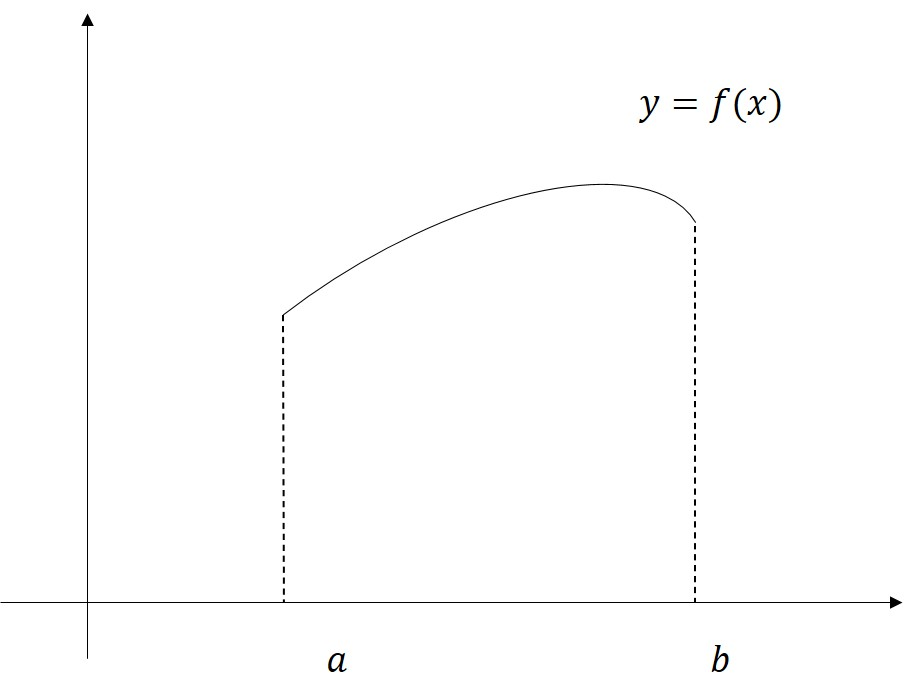
\includegraphics[width=5cm]{integracion1}
 	\caption{}
 	\label{integracion1}
 	
 \end{figure}
 \textbf{Integral de Riemann}\\
% Sea un acurva $ y=f(x) $
\begin{thm}
	Dado un intervalo cerrado $ [a,b] $, llamaremos partición de $ [a,b] $ a una colección finita de puntos $ P=\{x_{0}, x_{1},..., x_{n}\} $ que satisfacen 
	\[ a=x_{0}<x_{1}<x_{2}<...<x_{n}=b \]
	También se puede denotar como $ P=\{x_{i}\}_{i=0}^{n} $.
\end{thm}
\begin{thm}
	Dada una función $ f:[a,b]\rightarrow\mathbb{R} $, llamamos \textsl{suma integral} o \textsl{suma de Riemann} de $ f $, correspondiente a la partición $ P $, a la suma de la forma
	\[ \sigma(f,P,\{\xi_{i}\})=\sum_{i=1}^{n}f(\xi_{i})\delta x_{i} \]
	donde los $ \xi_{i} $ son puntos arbitratios ubicados en los intervalos $ [x_{i-1}, x_{i}], (i=1,...,n) $ y $ \delta x_{i}=x_{i}-x_{i-1} $ es la longitud de dicho intervalo.
\end{thm}
\begin{thm}
	Dada una función $ f:[a,b]\rightarrow\mathbb{R} $, se denomina límite de las sumas integrales $ \sigma(f,P,\{\xi_{i}\}) $ a un número real $ I $ que satisface:\\
	Cualquiera que sea $ \epsilon>0 $, existe una partición $ P_{\epsilon} $ de $ [a,b] $ para toda partición $ P $ más fina que $ P_{\epsilon} $ y toda colección de puntos $ \{\xi_{i}\} $ tiene lugar la desigualdad  
	\[ 	|\sigma(f,P,\{\xi_{i}\})-I|<\epsilon. \]
	Cuando $ I $ es el límite de las sumas integrales $ \sigma(f,P,\{\xi_{i}\}) $ se escribirá
	\[ \lim\limits_{\{P\}}\sigma(f,P,\{\xi_{i}\})=I \]
\end{thm}
\textbf{Definición de una integral según Riemann}\\
\begin{thm}
	La función $ f:[a,b]\rightarrow\mathbb{R} $, se llama \textsl{integrable} (seg\'un Riemann) o \textsl{R-integrable} en el intervalo $ [a,b] $ si sus sumas integrales tienen límite, esto es, si existe $ I\in\mathbb{R} $ tal que 
		\[ \lim\limits_{\{P\}}\sigma(f,P,\{\xi_{i}\})=I \]
		El número $ I $ es la \textsl{integral de f en el intevalo }[a,b] y se denota por
			\[ I=\lim\limits_{\{P\}}\sigma(f,P,\{\xi_{i}\})=\int_{a}^{b}f(x)dx \]
			La función f se denomina integrando y las cantidades a y b respectivamente límites
			inferior y superior de la integral.
\end{thm}
 Dada esta figura (\ref{integracion1}), se nos presenta el problema de calcular el área bajo la curva. Para lo cual se procede dividiendo la región en varios rectángulos de tamaño tan pequeños como se quiera, lógico de que a medida que estos pedacitos sean más pequeños es más exacta la aproximación.
 
 
 
 \begin{figure}[h]
 	\centering
 	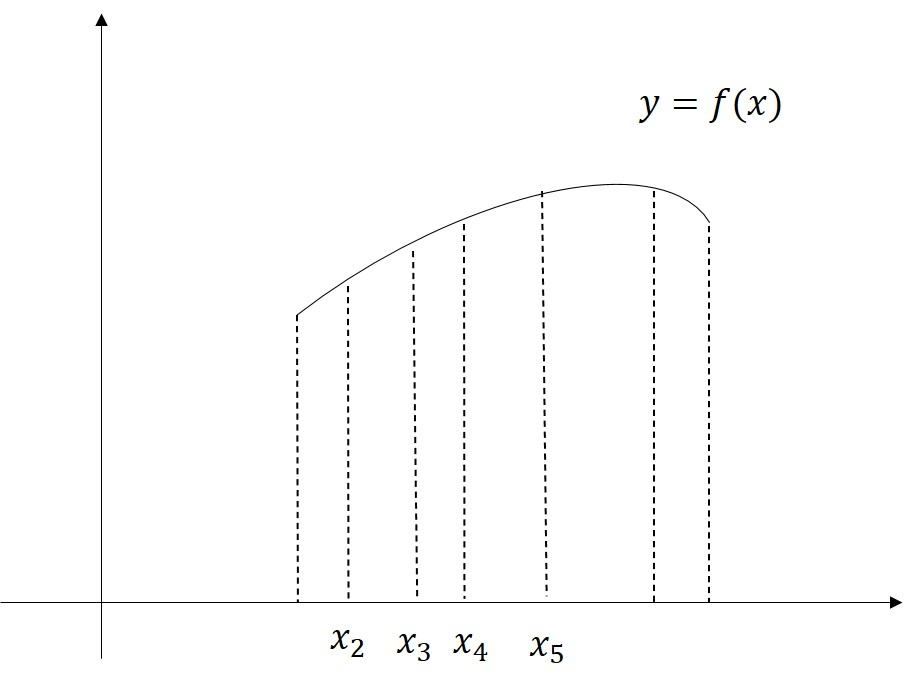
\includegraphics[width=5cm]{integracion2}
 	\caption{}
 	\label{integracion2}
 	
 \end{figure}
 El intervalo $ [a,b] $, es dividido en $ n $ partes iguales, con puntos $ a=x_{0}< x_{1}<...<x_{n}=b $, los cuales hacen que el intervalo quede de la siguiente forma dividido, por 
 \[ [x_{0}, x_{1}], [x_{1},x_{2}],...,[x_{n-1},x_{n}] \]
 Cada uno, de estos intervalos tiene un tamaño, es decir, un incremento que representa la distancia de un punto a otro.
 \[ \Delta x_{1}=x_{1}-x_{0} \]
 \[ \Delta x_{2}=x_{2}-x_{1} \]
 \[ ..... \]
 \[ \Delta x_{n}=x_{n}-x_{n-1} \]
 Ahora, si se toman puntos $ \xi_{i}\in[x_{i-1},x_{i}] $ con $ i=1,...,n $. 
 Se puede tener un valor estimado de la altura de cada sección de la figura en cuestión, y así calcular su área mediante una sumatoria del área de rectángulos (ver figura \ref{integracion3})
 \begin{figure}[h]
 	\centering
 	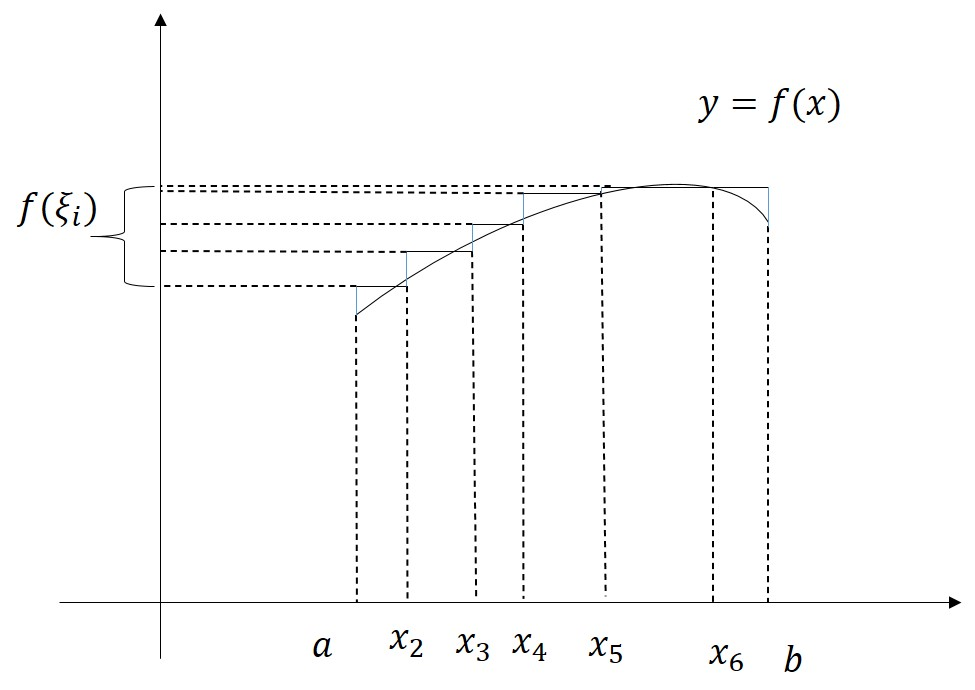
\includegraphics[width=5cm]{integracion3}
 	\caption{}
 	\label{integracion3}
 \end{figure}
 El área bajo la curva esta dada por la fórmula
 \begin{equation}
 	S_{n}=f(\xi_{1})\Delta x_{1}+f(\xi_{2})\Delta x_{2}+...+f(\xi_{n})\Delta x_{n}
 \end{equation}
 A medida que crece la cantidad de particiones, se hace más preciso el cálculo interal
 \begin{equation}
 	S=\lim\limits_{\Delta x\rightarrow0}f(\xi_{1})\Delta x_{1}+f(\xi_{2})\Delta x_{2}+...+f(\xi_{n})\Delta x_{n}
 \end{equation}
 Como se puede apreciar esta precisión se logra con el paso al límite. En este caso con: $ \Delta x\rightarrow0 $, se está haciendo más pequeño cada intervalo.
 \begin{equation}
 	S=\lim\limits_{\Delta x\rightarrow0}S_{n}
 \end{equation}
 \begin{equation}
 	S=\lim\limits_{\Delta x\rightarrow 0}\sum_{i=1}^{n}f(\xi_{i})\Delta x_{i}
 \end{equation}
 
 
   \begin{thm}
   	Una función $ f(x) $ se llama integrable en el intervalo $ [a,b] $, si existe el l\'imite finito $ I $ de la suma integral $ S_{n} $ de esta función cuando $ \Delta x\rightarrow0 $
   	\begin{equation}
   		I=\lim\limits_{\Delta x_{i}\rightarrow0}S_{n}=\lim\limits_{\Delta x_{i}\rightarrow0}\sum_{i=1}^{n}f(\xi_{i})\Delta x_{i}
   	\end{equation}
   	y este límite no depende del procedimiento de división del intervalo $ [a,b] $ en subintervalos ni de la elección de los puntos medios $ \xi_{i} $.\\
   	Este límite se llama integral definida de la función $ f(x) $ en el intervalo $ [a,b] $ y se denota por
   	\begin{equation}
   		 I=\int_{a}^{b}f(x)dx 
   	\end{equation}
   \end{thm}
En el proceso de definición de la integración definida, se utilizó una $ S $   para representar a las sumas, esta $ S $ se fue deformando hasta llegar a lo que ahora conocemos como el signo de integral $ \int $ que no es más que una $ S $ estilizada.\\
$ a $ y $ b $ son los límites de integración, y el resto $ f(x)dx $ la expresión integrando de la que ya se venía hablando.
 \begin{ejemplo}
 	Nos piden calcular el área de una función constante
 	\[ f(x)=c \]
 	en un intervalo $ [a,b] $.\\
 	Siguiendo el procedimiento anterior, 
 	\begin{enumerate}
 		\item Se forman las sumas $ S_{n} $.
 		\item Se buscan las $ f(\xi_{i}) $, que en este caso serán igual a $ c $ por ser función constante.
 		\item Se procede a calcular con la fórmula
 		\[ S_{n}=\sum_{i=1}^{n}c\Delta x_{i} \]
 		que por ser una funci\'on constante solo se tomará una partición (ver \ref{integracion5})
 	\end{enumerate}
 	\begin{equation}
 	S_{n}=c\sum_{i=1}^{n}\Delta x_{i}
 	\end{equation}
 	\begin{equation}
 	S_{n}=c\Delta x_{i}
 	\end{equation}
 	por ser solo una partición, $ \Delta x=b-a $
 	\begin{equation}
 	S_{n}=c(b-a)
 	\end{equation}
 	Y usando la definición
 	\[ I=\int_{a}^{b}dx=c(b-a) \]
 \end{ejemplo}
 
 

\begin{figure}[h]
	\centering
	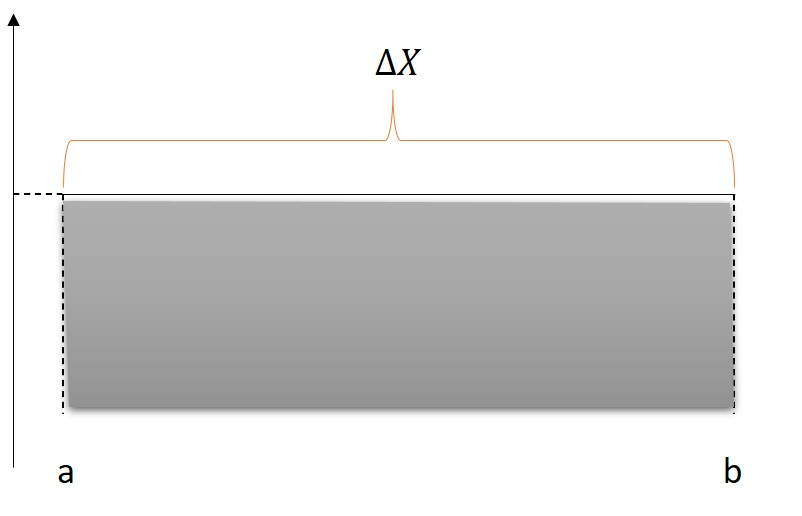
\includegraphics[width=7cm]{integracion5}
	\caption{Función lineal}
	\label{integracion5}
\end{figure}

    \begin{figure}[h]
    	\centering
    	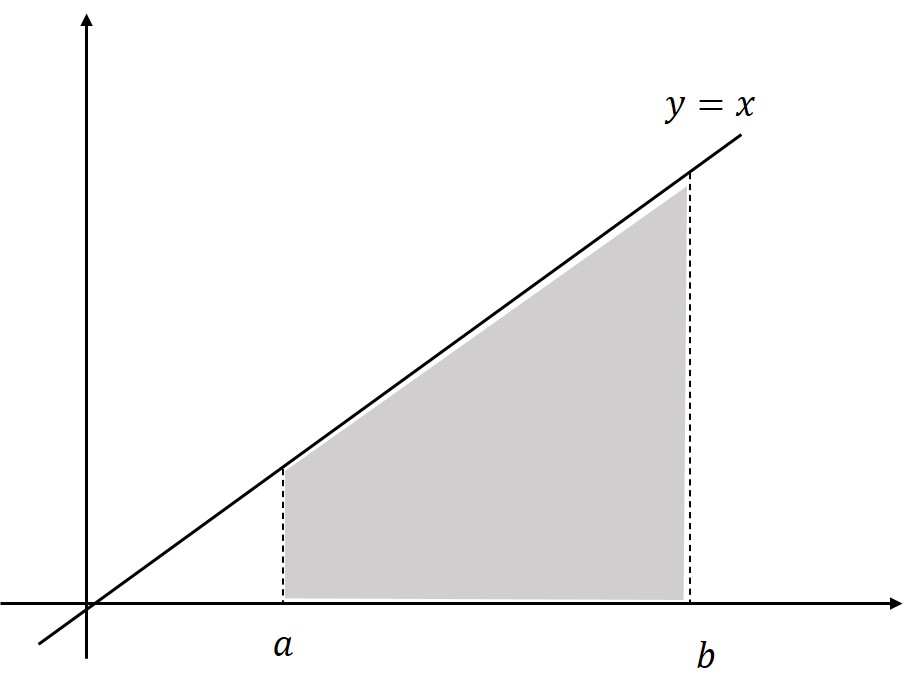
\includegraphics[width=5cm]{integracion4}
    	\caption{Función lineal}
    	\label{integracion4}
    \end{figure}
\begin{ejemplo}\label{calculo_area}
	Calcule el área bajo la curva de la función $ f(x)=x $ en el intervalo $ [a,b] $, ver figura (\ref{integracion4}).\\
	Para comenzar se divide el intervalo en partes iguales\\
	\[ h=\dfrac{b-a}{n} \]
Como nuestra función de interés es $ y=x $, el siguiente conjunto de valores:
	\[ a+h, a+2h, ..., a+(n-1)h \]
	La selección de intervalos es importante porque hace que sea más fácil o difícil el cálculo de las sumas. \\

	\begin{equation}\
	S_{n}=(a+h)\cdot h+(a+2h)\cdot h+...+(a+nh)\cdot h
	\end{equation}
	\begin{equation}
	=nah+(1+2+...+n)h^{2}
	\end{equation} 
	Recordar que la fórmula para calcular la sumatoria de un conjunto de números naturales 
	\[ \sum_{i=1}^{n}i=\dfrac{n(n+1)}{2} \]
	
	\begin{equation}
=nah+\dfrac{1}{2}n(n+1)h^{2}	
	\end{equation}
	sustituyendo $ h=\dfrac{b-a}{n} $
	\begin{equation}
	S_{n}=a(b-1)+\dfrac{1}{2}(1+1/n)(b-a)^{2}
	\end{equation}
	y como la integral es el siguiente límite
	\begin{equation}
	\int_{a}^{b}xdx=\lim\limits_{n\rightarrow\infty}S_{n}=\lim\limits_{n\rightarrow\infty}\left [a(b-a)+\dfrac{1}{2}(1+1/n)(b-a)^{2}\right]
	\end{equation}
	\begin{equation}
	=a(b-a)+\dfrac{1}{2}(b-a)^{2}
	\end{equation}
	Observese este resultado que no es coherente, de ahí la importancia de la selección de intervalos y puntos para conformar la suma.\\
	\textbf{Caso 2}\\
	Ya se sabe que 
	\[ [a,b]=\bigcup_{i=1}^{n}\left [a+\dfrac{b-a}{n}(i-1),a+\dfrac{b-a}{n}i\right ] \]
	Pero si en vez de calcularle el área a ese intervalo se la calculamos a uno que cominece desde $ o $
\[ 	\left [0,\dfrac{b-a}{n}\right ]=\bigcup_{i=1}^{n}\left [\dfrac{b-a}{n}(i-1),\dfrac{b-a}{n}i\right ] \]
\begin{equation}
\sum_{i=1}^{n}f(x_{i})\Delta x
\end{equation}
es la f\'ormula  que estamos usando, y para este caso, se calculará una suma que acote inferiormente a la integral
\begin{equation}
\sum_{i=1}^{n}\dfrac{b-a}{n}(i-1)\dfrac{b-a}{n}
\end{equation}
\begin{equation}
=\sum_{i=1}^{n}\dfrac{(b-a)^{2}}{n^{2}}(i-1)
\end{equation}
\begin{equation}
=\dfrac{(b-a)^{2}}{n^{2}}\sum_{i=1}^{n}(i-1)
\end{equation}
Las series $ \sum_{i=1}^{n}(i-1)=n+\dfrac{(n+1)n}{2} $
\begin{equation}
=\dfrac{(b-a)^{2}}{n^{2}}\left [\dfrac{n^{2}+n}{2}+n\right ]
\end{equation}
\begin{equation}
=\dfrac{(b-a)^{2}}{2}+\dfrac{(b-a)^{2}}{2n}+\dfrac{(b-a)^{2}}{n}
\end{equation}
que calculando el límite de $ n\rightarrow\infty $
\begin{equation}
\lim\limits_{n\rightarrow\infty}\left [\dfrac{(b-a)^{2}}{2}+\dfrac{(b-a)^{2}}{2n}+\dfrac{(b-a)^{2}}{n}\right ]=\dfrac{(b-a)^{2}}{2}
\end{equation}
De esta forma se ha calculado la integral de una curva $ f(x)=x $ en  el intervalo $ [0,b-a] $; que no es más que el área del mismo triángulo, lo que trasladado, es decir, sin el cuadrado que esta abajo. (Ver \ref{integracion6}). Para completar lo que le falta se le suma a este resultado $ (b-a)a=ab-a^{2} $ el área del rectángulo.
    \begin{figure}[h]
    	\centering
    	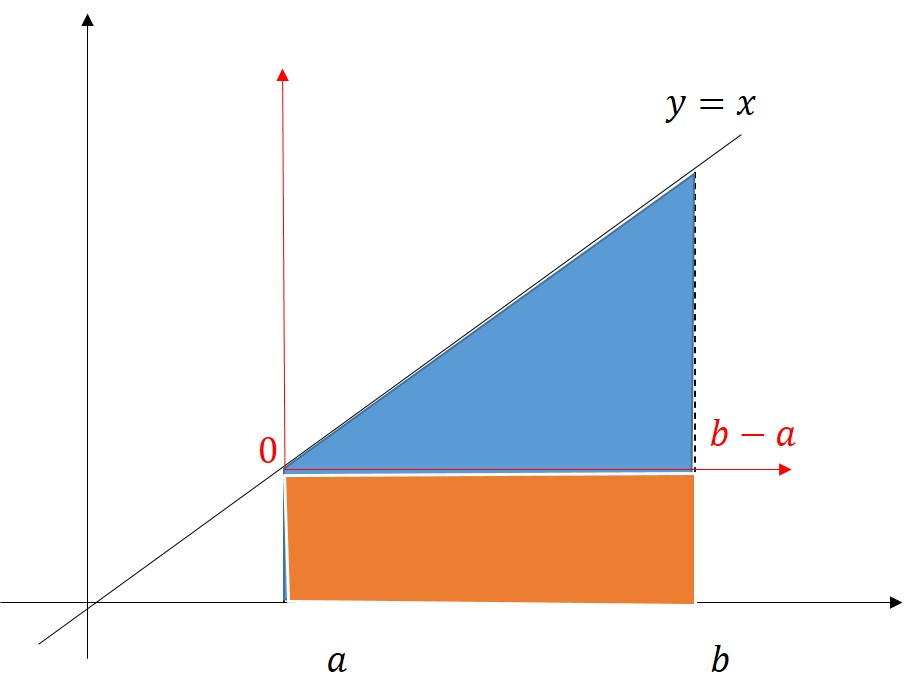
\includegraphics[width=5cm]{integracion6}
    	\caption{Función lineal}
    	\label{integracion6}
    \end{figure}
 Entonces el área bajo la curva será 
 \begin{equation}
 A=\dfrac{(b-a)^{2}}{2}+ab-a^{2}
 \end{equation} 
 \begin{equation}
 A=\dfrac{b^{2}+a^{2}}{2}-ab+ab-a^{2}
 \end{equation}   
\begin{equation}
 A=\dfrac{b^{2}+a^{2}}{2}-a^{2}
\end{equation}    
\begin{equation}
 A=\dfrac{b^{2}-a^{2}}{2}
\end{equation}
que es el área de la función en cualquier intervalo $ [a,b] $.\\

\end{ejemplo}
¿Es un trabajo tedioso? \\
Claro que si!!\\




\textbf{Propiedades fundamentales de la integral definida}\\
\begin{enumerate}
	\item $ \int_{a}^{b}kf(x)dx=k\int_{a}^{b}f(x)dx $
	\item $ \int_{a}^{b}[f(x)\pm g(x)]dx=\int_{a}^{b}f(x)dx\pm \int_{a}^{b}g(x)dx $
	\item $ \int_{a}^{b}f(x)dx=\int_{a}^{c}f(x)dx+\int_{c}^{b}f(x)dx $
	\item  Si en $ [a,b] $ $ a<b $, y $ f $ y $ g $ son integrrables con $ f(x)\leq g(x) $ entonces
	\[ \int_{a}^{b}f(x)dx\leq \int_{a}^{b}g(x)dx \]
	\item Teorema del valor medio del cálculo integral(ver en anexos) \\
	Si $ f\in R[a,b] $, Riemann intergable, y $ m,M $ extremos inferior y superior recpectivamente, de $ f(x) $ en $ [a,b] $,
	\textbf{entonces} exite un $ \mu $ tal que 
	\begin{enumerate}
		\item $ m\leq\mu\leq M $
		\item $ \int_{a}^{b}f(x)dx=\mu(b-a) $
	\end{enumerate}
	Si además $ f(x) $ se supone continua, existe $ c\in[a,b] $ tal que $ f(c)=\mu $.
\begin{equation}
	\int_{a}^{b}f(x)dx=\mu(b-a)=f(c)(b-a)
\end{equation}
	\begin{equation}
\int_{a}^{b}mdx\leq\int_{a}^{b}f(x)dx\leq\int_{a}^{b}Mdx
	\end{equation}
\end{enumerate}
















 \subsubsection{Primer y segunto teorema del cálculo interal. Problemas de Cálculo de área.}
La relación entre integral y derivada es fundamental para comprender el siguiente resultado. Para ver ello se comienza con el análisis de definida con límite superior variable
\[ F(x)=\int_{a}^{x}f(t)dt \]
Con tener a $ f $ integrable se cumple que 
\begin{equation}
\displaystyle F(x_{0}+\Delta x)-F(x_{0})=\int_{a}^{x+\Delta x}f(t)dt=\mu_{\Delta x}\Delta x
\end{equation}
que se puede llevar a la forma
\begin{equation}
\displaystyle \dfrac{F(x_{0}+\Delta x)-F(x_{0})}{\Delta x}=\dfrac{1}{\Delta x}\int_{a}^{x+\Delta x}f(t)dt=\mu_{\Delta x}
\end{equation}
donde 
\[ m_{\Delta x}\leq \mu_{\Delta x\leq M_{\Delta x}} \]
Que son los ínfimos, valor medio y supremo, respectivamente en ese intervalo de $ f(x) $. Y por conocimientos previos ya sabemos que todo depende de la existencia del límite de $ \mu_{\Delta x} $ cuando $ \Delta x\rightarrow0 $. \\
Verifiquemos si $ f $ es continua en $ x_{0} $, entonces
\[ \lim\limits_{\Delta x\rightarrow0}m_{\Delta x}=\lim\limits_{\Delta x\rightarrow0}M_{\Delta x}=f(x_{0}) \]
y por lo tanto, también $ \lim\limits_{\Delta \rightarrow0}\mu_{\Delta x}=f(x_{0}) $.
\\Por definicón  de $ M_{\Delta x} $, se cumple que $ f(x_{0})\leq M_{\Delta x} $ y además, para cualquier $ \epsilon>0 $, existe algún $ x'\in[x_{0},x_{0}+\Delta x] $ tal que 
\[ f(x')>M_{\Delta x}-\epsilon \]


 \begin{figure}[h]
 	\centering
 	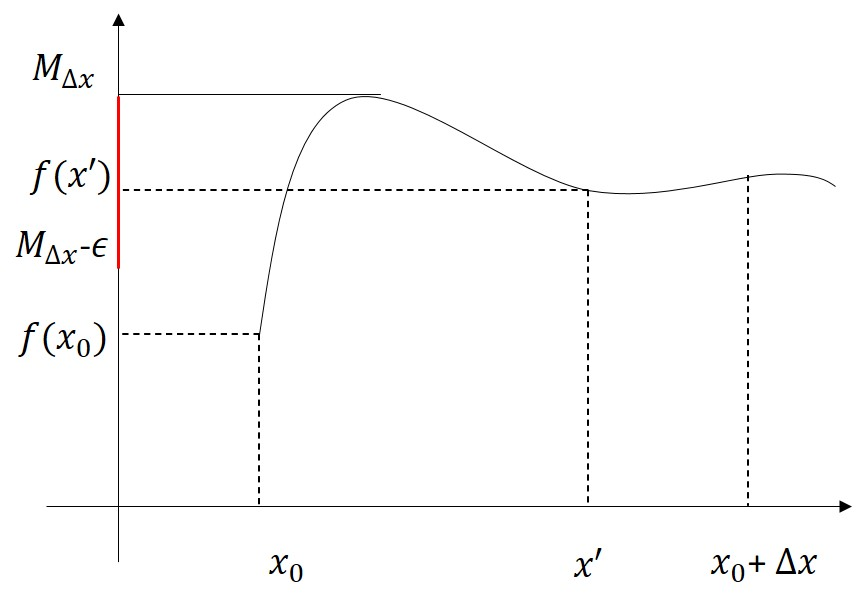
\includegraphics[width=5cm]{integracion7}
 	\caption{}
 	\label{integracion7}
 \end{figure}






\begin{equation}
0\leq M_{\Delta x}-f(x_{0})=M_{\Delta x}-f(x')+(f(x')-f(x_{0})\leq M_{\Delta x}-f(x')+|f(x')-f(x_{0})|<\epsilon+|f(x')-f(x_{0})|
\end{equation}
La continuidad de $ f $ en $ x_{0} $ asegura la existencia de algún $ \delta>0  $ tal que para $ |\Delta x|<\delta $ y $ x'\in [x_{0}, x_{0}+\Delta x] $ se cumple que 
\begin{equation}
|f(x')-f(x_{0})|<\epsilon
\end{equation}
Así hemos demostrado que $ |\Delta x|<\delta $ tine lugar la desigualdad 
\begin{equation}
0\leq M_{\Delta x}-f(x_{0})\leq 2\epsilon
\end{equation}
es decir 
\begin{equation}
\lim\limits_{\Delta x\rightarrow0}M_{\Delta x}=f(x_{0})
\end{equation}
De forma análoga se prueba que $ \lim\limits_{\Delta x\rightarrow0}m_{\Delta x}=f(x_{0}) $, por consiguiente $ \lim\limits_{\Delta x\rightarrow0}\mu_{\Delta x}=f(x_{0}) $, luego $ F $ es derivable en  $ x_{0} $ y $ F'(x_{0})=f(x_{0}) \blacksquare$




 \begin{teorema}
 	\textbf{Primer teorema fundamental del cálculo integral}\\
 	Si $ f $ es continua en $ [a,b] $ y $ F(x)=\int_{a}^{x}f(t)dt $ entonces $ F(x) $ es derivable en $ (a,b) $ y para todo $ x\in(a,b) $ 
 	\begin{equation}
 	F'(x)=f(x)
 	\end{equation}
 \end{teorema} 
 Una consecuencia muy importante es que toda función continua tiene primitiva.
 
 
 \begin{teorema}
 	\textbf{Segundo Teorema Fundamental del Cálculo integral}\\
 	Si $ f  $ es continua en $ [a,b] $ y $ F(x) $ es una primitiva cualquiera cualquiera de $ f(x) $, entonces:
 	\begin{equation}
 	\int_{a}^{b}f(x)dx=F(b)-F(a)=F(x)\bigg|_{a}^{b}
 	\end{equation}
 \end{teorema}
 Esta fórmula también es conocida como la fórmula de Newton-Leibniz, por el gran aporte hecho de estos dos grandes matem\'aticos.
 
 
 \textbf{Demostración}\\
 Sea $ G $ y $ F $ primitivas de $ f $ en un intervalo $ [a,b] $
 \begin{equation}
 G(x)=F(x)+C\;\;\;\;\;\;	\mbox{para $ x\in [a,b] $}
 \end{equation}
con   $ C $ constante. \\
 Recordar que ya teníamos
\[ F(x) =\int_{a}^{x}f(t)dt \]

Entonces se cumple que
\begin{equation}
	\int_{a}^{x}f(t)dt=G(x)+C\label{teorema_fundamental_calculo}
\end{equation}

 Evaluando $ x=a $ en (\ref{teorema_fundamental_calculo})%y $ x=b $ obtenemos
\begin{equation}
	\int_{a}^{a}f(t)dt=G(a)+C
\end{equation}
 Pero $ \int_{a}^{a}f(t)dt=0 $, la demostración es sencilla solo hay que usar las sumas integrales de Riemann con todos los $ \Delta x=0 $ que harían el resultado nulo.\\
 Entonces
 \begin{equation}
0=G(a)+C
 \end{equation}
 \begin{equation}
C=-G(a)
 \end{equation}
 Este último resultado es útil porque ya en lo sucesivo no se empleará mas la constante. Para $ x=b $ en (\ref{teorema_fundamental_calculo}) se hace lo mismo 
 \begin{equation}
 	\int_{a}^{b}f(t)dt=G(b)-G(a)
 \end{equation}
 que es el resultado de este importantísimo teorema, el cual nos da la facilidad de, con obtener la primitiva de una función y evaluar el valor inicial y el final del segmento en la fórmula se tiene el área bajo la curva.
% \;\;\;\;\mbox{y}\;\;\;\; G(b)=F(b)+C \]
 
\begin{ejemplo}
	Calcule $ \int_{0}^{1}\dfrac{dx}{1+x^{2}} $
	\begin{equation}
	\int_{0}^{1}\dfrac{dx}{1+x^{2}}=\arctan x\bigg|_{0}^{1}=\arctan(1)-\arctan(0)=\dfrac{\pi}{4}
	\end{equation}
\end{ejemplo} 
Hagamos una pequeña comparación, con el ejemplo (\ref{calculo_area})
\begin{ejemplo}
	\[ \int_{a}^{b}xdx \]
	Es sabido de las integrales indefinidas que
	\[ \int xdx=\dfrac{x^{2}}{2}+c \]
	Ahora con el (\ref{teorema_fundamental_calculo})
\begin{equation}
	\int_{a}^{b}xdx=\dfrac{x^{2}}{2}\bigg|_{a}^{b}=\dfrac{b^{2}-a^{2}}{2}
\end{equation}
\end{ejemplo}
No hay comparación con lo que se ahorra.





 \subsubsection{Integrales impropias}
 
 \begin{thm}
 	Si existe el límite finito
 	\begin{equation}
 	\lim\limits_{b\rightarrow\infty}\int_{a}^{b}f(x)dx
 	\end{equation}
 	Este límite se llama integral impropia de primera especie de la función $ f(x) $ en el intervalo $ [a,\infty) $ y se designa por 
 	\begin{equation}
 	\int_{a}^{\infty}f(x)dx=\lim\limits_{b\rightarrow\infty}\int_{a}^{b}f(x)dx
 	\end{equation}
 	en este caso es convergente, de lo contrario sería divergente.
 \end{thm}
 Otra forma de ver el mismo tipo de integral es la siguiente:
 \begin{equation}
 \int_{-\infty}^{b}f(x)dx=\lim\limits_{a\rightarrow-\infty}\int_{a}^{b}f(x)dx
 \end{equation}
 \begin{equation}
\int_{\infty}^{\infty}f(x)dx=\lim\limits_{u\rightarrow\infty}\int_{0}^{u}f(x)dx+\int_{-u}^{0}f(x)dx
 \end{equation}
\begin{ejemplo}
Calcular $ 	\int_{0}^{\infty}\dfrac{dx}{1+x^{2}} $
\begin{equation}
=	\lim\limits_{b\rightarrow\infty}\int_{0}^{b}\dfrac{dx}{1+x^{2}} 
\end{equation}
como se pudo ver, la integral impropia se transformó en una integral propia, con la cual ya se sabe trabajar
\begin{equation}
=	\lim\limits_{b\rightarrow\infty}(\arctan b- \arctan 0)
\end{equation}
\begin{equation}
=	\lim\limits_{b\rightarrow\infty}\arctan b=\dfrac{\pi}{2}
\end{equation}
\end{ejemplo}

Por otro lado están las integrales impropias de segunda especie son integrales que se caracterizan por tener una discontinuida de salto infinito dentro del intervalo de integración de la función integrando.
\begin{thm}
	Si existe el límite finito
	\[ 
	\lim\limits_{\epsilon\rightarrow+0}\int_{a}^{b-\epsilon}f(x)dx
	 \]
	 este límite se llama integral impropia de segunda especie de la función $ f(x) $ en el intervalo $ (a,b) $ y se denota por
	 \begin{equation}
	int_{a}^{b}f(x)dx=\lim\limits_{\epsilon\rightarrow+0}\int_{a}^{b-\epsilon}f(x)dx
	 \end{equation}
\end{thm}
\begin{ejemplo}
	Calcula:
	\[ \int_{0}^{1}\dfrac{dx}{\sqrt{1-x^{2}}} \]
	hay que notar que en $ x=1 $ la función se hace discontinua y por lo tanto 
	\[  \lim\limits_{x\rightarrow1}\dfrac{1}{\sqrt{1-x^{2}}}=\infty \]
	\begin{equation}
	\int_{0}^{1}\dfrac{dx}{\sqrt{1-x^{2}}}= \lim\limits_{\epsilon\rightarrow0+}\int_{0}^{1-\epsilon}\dfrac{dx}{\sqrt{1-x^{2}}}
	\end{equation}
	\begin{equation}
	=\lim\limits_{\epsilon\rightarrow0+}(\arcsin x)\biggl|_{0}^{1-\epsilon}=\arcsin1-\dfrac{\pi}{2}
	\end{equation}
\end{ejemplo}










 \subsection{Ejercicios Resueltos}
\textbf{Integral indefinida}\\
\begin{enumerate}
	


\item Calcule
\begin{enumerate}
	

\item[a)] $  \int(5x^{4}-8x^{3}+9x^{2}-2x+7)dx  $\\
y aplicando las propiedades de la integral se tiene
\begin{equation}
= 5\int x^{4}dx-8\int x^{3}dx+9\int x^{2}dx-2\int xdx+7\int dx
\end{equation}
que luego integrando
\begin{equation}
= 5\dfrac{x^{5}}{5}-8 \dfrac{x^{4}}{4}+9 \dfrac{x^{3}}{3}-2 \dfrac{x^{2}}{2}+7x+c
\end{equation}
\begin{equation}
= x^{5}-2x^{4}+3x^{3}-2 x^{2}+7x+c
\end{equation}
\item[b)] $ \int \sqrt{x}\left (x+\dfrac{1}{x}\right )dx $\\
con el uso de las propiedades de la potencia se tiene
\begin{equation}
=\int x^{1/2}(x+x^{-1})dx
\end{equation}
\begin{equation}
=\int (x^{3/2}+x^{-1/2})dx
\end{equation}
e integrando
\begin{equation}
=\dfrac{x^{5/2}}{5/2}+\dfrac{x^{1/2}}{1/2}+c
\end{equation}
\begin{equation}
=\dfrac{2}{5}x^{5/2}+2\sqrt{x}+c
\end{equation}


\item[c)] $ \int (3\sin t-2\cos t)dt $
aplicando las propiedades
\begin{equation}
=3\int\sin tdt-2\int\cos tdt
\end{equation}
integrando
\begin{equation}
=3(-\cos t)-2\sin t+c=-3\cos t-2\sin t+c
\end{equation}
\end{enumerate}


\textbf{Integración por cambio de variables}\\

\item Calcule
\begin{enumerate}
	\item[a)] $ \int\sqrt{3x+4}dx $
	Comenzamos usando las propiedades de la potencia
	\begin{equation}
	\int(3x+4)^{1/2}dx
	\end{equation}
	\[ \phi=3x+4 \]
	\[ d\phi=3dx\Rightarrow dx=\dfrac{d\phi}{3} \]
	efectuando el cambio de variables
	\begin{equation}
	=\int(\phi)^{1/2}\dfrac{d\phi}{3}
	\end{equation}
	por propiedades de la derivada
	\begin{equation}
	=\dfrac{1}{3}\int(\phi)^{1/2}d\phi
	\end{equation}
	integrando
	\begin{equation}
	=\dfrac{1}{3} \dfrac{\phi^{3/2}}{3/2}+c 
	\end{equation}
	\begin{equation}
	=\dfrac{2}{9}\phi^{3/2}+c 
	\end{equation}
	volviendo a realizar el cambio de variables
	\begin{equation}
		=\dfrac{2}{9}(3x+4)^{3/2}+c
	\end{equation}
	
	\item[b)] $ \int \dfrac{\sin \sqrt{x}}{\sqrt{x}}dx $
	\[ \varphi=\sqrt{x} \]
	\[ d\varphi=\dfrac{1}{2\sqrt{x}} \Rightarrow 2d\varphi=\dfrac{dx}{\sqrt{x}}\]
	efectuando el cambio de variable se tiene 
	\begin{equation}
	\int \dfrac{\sin \varphi d\varphi}{2}=-2\cos \varphi+c
	\end{equation}
	\begin{equation}
	=-2\cos \sqrt{x}+c
	\end{equation}
	
























\textbf{Integración por partes}\\
\item [3)]Calcula
\begin{enumerate}
	\item[a)] $ \displaystyle\int \sin^{2} xdx $
	\item[b)] $ \displaystyle\int\ln xdx $
	\item[c)] $ \displaystyle\int x\sqrt{1+x}dx $
\end{enumerate}
\textbf{Solución}\\
\begin{enumerate}
	\item[a)] \begin{equation}
	\displaystyle\int \sin^{2} xdx
	\end{equation}
	\[ \begin{array}{cc}
	u=\sin x & dv=\sin xdx\\
	du =\cos x dx & v=-\cos x
	\end{array} \]
	\begin{equation}
	=\sin x(-\cos x)-\int \cos x(-cos x)dx=-\sin x\cos x+\int \cos^{2}dx
	\end{equation}
	Como $ \cos^{2}x=1-\sin^{2} x $
	\begin{equation}
	=-\sin x\cos x+\int (1-\sin^{2})dx
	\end{equation}
	\begin{equation}
	=-\sin x\cos x+\int dx-\int\sin^{2}dx	=-\sin x\cos x+x-\int\sin^{2}dx
	\end{equation}
	si nos percatamos, esta integral se repite el mismo resultado al usar el método de integración por partes
	\begin{equation}
	\int\sin^{2}dx=-\sin x\cos x+x-\int\sin^{2}dx
	\end{equation}
	pasando para el miembro izquierdo $ -\int\sin^{2}dx $
	\begin{equation}
	2\int\sin^{2}dx=-\sin x\cos x+x+c
	\end{equation}
	\begin{equation}
	\int\sin^{2}dx=\dfrac{-\sin x\cos x+x}{2}+c\blacksquare
	\end{equation}
	 \item[b)] \begin{equation}
	  \displaystyle\int\ln xdx
	 \end{equation}	
	 \[ \begin{array}{cc}
	 u=\ln x & dv=dx\\
	 du=\dfrac{dx}{x} & v=x
	 \end{array} \]
	 \begin{equation}
	 =x\ln x-\int x\dfrac{dx}{x}
	 \end{equation}
	 \begin{equation}
	 	 =x\ln x-\int dx
	 \end{equation}
	 \begin{equation}
	 	 	 =x\ln x-x+c\blacksquare
	 \end{equation}
	\item[c)] \begin{equation}
	\displaystyle\int x\sqrt{1+x}dx
	\end{equation}
\[ \begin{array}{cc}
u=x & dv=\sqrt{1+x}dx\\
du=dx & v=2\dfrac{(1+x)^{3/2}}{3}
\end{array} \]
\begin{equation}
=\dfrac{2x}{3}(1+x)^{3/2}-\dfrac{2}{3}\int (1+x)^{3/2}dx
\end{equation}
\begin{equation}
=\dfrac{2x}{3}(1+x)^{3/2}-\dfrac{2}{3} \dfrac{(1+x)^{5/2}}{5/2}+c
\end{equation}
\begin{equation}
=\dfrac{2x}{3}\sqrt{(1+x)^{3}}-\dfrac{4}{15} \sqrt{(1+x)^{5}}+c\blacksquare
\end{equation}
\end{enumerate}




\textbf{Integración por fracciones simples}\\
\item[4)] Calcular
\begin{enumerate}
	\item[a)] $ \int \dfrac{x-4}{x^{3}-x^{2}-x-2}dx $
	\textbf{Solución:}\\
	\begin{equation}
	=\int \dfrac{x-4}{(x-2)(x^{2}+x+1)}dx
	\end{equation}
	Pero para simplificar el trabajo se tomará la función integrando $ \dfrac{x-4}{(x-2)(x^{2}+x+1)} $ y se descompondrá en fracciones más simples
\[ 	\dfrac{x-4}{(x-2)(x^{2}+x+1)}= \dfrac{A}{x-2}+\dfrac{Bx+C}{x^{2}+x+1}\]
Se juntan las racciones para buscar los coeficientes
\[  	\dfrac{x-4}{(x-2)(x^{2}+x+1)}=\dfrac{A(x^{2}+x+1)+(Bx+C)}{(x-2)(x^{2}+x+1)} \]
y se llaga a la coclusi\'on de que
	\[ x-4=A(x^{2}+x+1)+(Bx+C) \]
	\[ x-4=(A+B)x^{2}+(A-2B+C)x+A-2C \]
	En este caso se opta por calcular las constantes indeterminadas igualando los coeficientes de los términos del mismo grado en ambos miembros\\
	$  x^{2}:\;\;\;\;0=A+B  $\\
$ 	 x:\;\;\;\;\;\;1=A-2B+C $ \\
$ 	 1:\;\;\;\;\;\;-4=A-2C  $\\
De donde se deduce que 
\[ B=-A, \;\;\;\; C=2+\dfrac{A}{2} \]
sustituyendo y calculando se obtiene que $ A=-\dfrac{2}{7} , B=\dfrac{2}{7}, C=\dfrac{13}{7}$, entonces, la fracción simple queda de la siguiente forma
\[ \dfrac{x-4}{(x-2)(x^{2}+x+1)}=-\dfrac{2}{7}\dfrac{1}{x-2}+\dfrac{\dfrac{2}{7}x+\dfrac{13}{7}}{x^{2}+x+1}  \]
volviendo a la integral
\begin{equation}
\int\dfrac{x-4}{(x-2)(x^{2}+x+1)}dx=\int-\dfrac{2}{7}\dfrac{1}{x-2}dx+\int\dfrac{\dfrac{2}{7}x+\dfrac{13}{7}}{x^{2}+x+1}dx
\end{equation}
\begin{equation}
=\dfrac{1}{7}\int\dfrac{-2}{x-2}dx+\dfrac{1}{7}\int\dfrac{2x+13}{x^{2}+x+1}dx
\end{equation}
\begin{equation}
=\dfrac{-2}{7}\ln|x-2|+\dfrac{1}{7}\int\dfrac{2x+13}{x^{2}+x+1}dx
\end{equation}
Para calcular a la otra integral que llamaremos $ I $
\begin{equation}
I=\dfrac{1}{7}\int\dfrac{2x+13}{x^{2}+x+1}dx=\dfrac{1}{7}\int\dfrac{2x+1+12}{x^{2}+x+1}dx
\end{equation}
\begin{equation}
I=\dfrac{1}{7}\int\dfrac{2x+1}{x^{2}+x+1}dx+\dfrac{1}{7}\int\dfrac{12}{x^{2}+x+1}dx
\end{equation}
Por un lado $ \int\dfrac{2x+1}{x^{2}+x+1}dx=\ln|x^{2}+x+1|+c $ integrando por sustituci\'on, y por el otro se hace un completamiento cuadr\'atico con $ x^{2}+x+1=x^{2}+x+1/4-1/4+1 $
\begin{equation}
I=\dfrac{1}{7}\ln|x^{2}+x+1|+\dfrac{12}{7}\int\dfrac{dx}{x^{2}+x+1/4+3/4}
\end{equation}
\begin{equation}
I=\dfrac{1}{7}\ln|x^{2}+x+1|+\dfrac{12}{7}\int\dfrac{dx}{(x+1/2)^{2}+3/4}
\end{equation}
Con el fin de convertir la segunda integral en lo más parecido a $ \arctan x $ compuesta por otra funci\'on
\begin{equation}
I=\dfrac{1}{7}\ln|x^{2}+x+1|+\dfrac{12}{7}\int\dfrac{dx}{3/4\left [\dfrac{(x+1/2)^{2}}{3/4}+1\right ]}
\end{equation}
como $ \dfrac{(x+1/2)^{2}}{3/4}=\left (\dfrac{2x}{\sqrt{3}}+\dfrac{1}{\sqrt{3}}\right )^{2} $
\begin{equation}
I=\dfrac{1}{7}\ln|x^{2}+x+1|+\dfrac{12}{7}\int\dfrac{dx}{3/4\left [\left (\dfrac{2x}{\sqrt{3}}+\dfrac{1}{\sqrt{3}}\right )^{2}+1\right ]}
\end{equation}
\begin{equation}
I=\dfrac{1}{7}\ln|x^{2}+x+1|+\dfrac{16}{7}\int\dfrac{dx}{\left (\dfrac{2x}{\sqrt{3}}+\dfrac{1}{\sqrt{3}}\right )^{2}+1}
\end{equation}
e integrando por el método de sustitución
\begin{equation}
I=\dfrac{1}{7}\ln|x^{2}+x+1|+\dfrac{16}{7}\frac{\sqrt{3}}{2}\arctan \left (\dfrac{2x+1}{\sqrt{3}}\right )+c\blacksquare
\end{equation}
y nuestro resultado final es 
\begin{equation}
\dfrac{-2}{7}\ln|x-2|+\dfrac{1}{7}\ln|x^{2}+x+1|+\dfrac{8\sqrt{3}}{7}\arctan\left  (\dfrac{2x+1}{\sqrt{3}}\right )+c
\end{equation}
\item [b)]$ \int \dfrac{2x+1}{x^{2}+x-2}dx $\\
\textbf{Solución:}\\
Es una fracción  racional propia. Su denominador tiene dos raíces reales simples
\[ x^{2}+x-2=(x+2)(x-1) \]
Así podemos plantear la descomposición:
\[ \dfrac{2x+1}{x^{2}+x-2}=\dfrac{A}{x+2}+\dfrac{B}{x-1} \]
Para hallar los valores de los coeficientes
\[ 2x+1=A(x-1)+B(x+2) \]
para $ x=1 $ se tiene $ 3=3B $, entonces $ B=1 $.\\
Y para $ x=-2 $, $ -3=-3A $ y $ A=1 $. Esta es una vía muy cómoda para este caso en que hay dos coeficientes con raíces reales.
\[ \dfrac{2x+1}{x^{2}+x-2}=\dfrac{1}{x+2}+\dfrac{1}{x-1} \]
La integral viene quedando de la siguiente forma
\begin{equation}
\int\dfrac{2x+1}{x^{2}+x-2}dx=\int\dfrac{A}{x+2}dx+\int\dfrac{B}{x-1} dx
\end{equation}
\begin{equation}
=\ln|x+2|+\ln|x-1|+c=\ln|(x+2)(x-1)|+c\blacksquare
\end{equation}
\item [c)]$ \displaystyle\int\dfrac{x+2}{x^{2}-4x+4}dx $\\
$ \dfrac{x+2}{x^{2}-4x+4} $ es una fracción racional propia, su denominador tiene la raíz $ x=2 $ de orden $ 2 $,  por lo tanto la descomposición será: $ x^{2}-4x+4=(x-2)^{2} $
\begin{equation}
\dfrac{x+2}{x^{2}-4x+4}=\dfrac{A}{(x-2)^{2}}+\dfrac{B}{x-2}
\end{equation}
En este caso no se puede emplear el método anterior, por tener las mismas ra\'ices cada factor
\[ x+2=A+B(x-2) \]
\[ x+2=A+Bx-2B) \]
Aquí es útil el método de coeficientes indeterminados\\
$ x: 1=B $\\
$ 1:2=A-2B $\\
Entonces $ A=4 $ y $ B=1 $
\begin{equation}
\dfrac{x+2}{x^{2}-4x+4}=\dfrac{4}{(x-2)^{2}}+\dfrac{1}{x-2}
\end{equation}
Integrando ambos miembros se obtiene
\begin{equation}
\int\dfrac{x+2}{x^{2}-4x+4}dx=\int\dfrac{4}{(x-2)^{2}}dx+\int\dfrac{1}{x-2}dx
\end{equation}
\begin{equation}
=-\dfrac{4}{x-2}+\ln|x-2|+c
\end{equation}
\item [d)]$ \int \dfrac{x+1}{(x^{2}+1)(x^{2}+2)}dx $
en este caso $ \dfrac{x+1}{(x^{2}+1)(x^{2}+2)}dx $ es propia y el denominador tiene dos pares de ra\'ices complejas y conjugadas simples
\[ \dfrac{x+1}{(x^{2}+1)(x^{2}+2)}=\dfrac{Ax+B}{x^{2}+1}+\dfrac{Cx+D}{x^{2}+2} \]
\[ x+1=(Ax+B)(x^{2}+2)+(Cx+D)(x^{2}+1) \]
Multiplicando y agrupando
\[ x+1=(A+C)x^{3}+(B+D)x^{2}+(2A+C)x+(2B+D) \]
de ahí se obtiene
\[ 
\begin{array}{cccc}
A+C=0\\
B+D=0\\
2A+C=1\\
2B+D=1\\
\end{array}
 \]
 La solución será $ A=1, B=1, C=-1, D=-1 $.
 \[ \dfrac{x+1}{(x^{2}+1)(x^{2}+2)}=\dfrac{x+1}{x^{2}+1}+\dfrac{-x-1}{x^{2}+2}  \]
 Planteando la integral
 \begin{equation}
  \int\dfrac{x+1}{(x^{2}+1)(x^{2}+2)}dx=\int\dfrac{x+1}{x^{2}+1}dx+\int\dfrac{-x-1}{x^{2}+2}dx
 \end{equation}
 Descomponiendo las integrales
 \begin{equation}
=\int\dfrac{x}{x^{2}+1}dx+\int\dfrac{1}{x^{2}+1}dx-\int\dfrac{x}{x^{2}+2}dx-\int\dfrac{1}{x^{2}+2}dx
 \end{equation}
 Aplicando sustitución en la primera y la tercera y en el resto se obtendrá como primitiva a $ \arctan \varphi $
 \begin{equation}
 =1/2\ln|x^{2}+1|+\arctan x-1/2\ln|x^{2}+2|-\dfrac{1}{\sqrt{2}}\arctan\dfrac{x}{\sqrt{2}}+C
 \end{equation}
 \begin{equation}
 =1/2\ln\bigg|\dfrac{x^{2}+1}{x^{2}+2}\bigg|+\arctan x-\dfrac{1}{\sqrt{2}}\arctan\dfrac{x}{\sqrt{2}}+C\blacksquare
 \end{equation}
 
\end{enumerate}

\end{enumerate}




\textbf{Teoremas fundamentales del cálculo intergal}\\
\item Una herida está sanando de forma tal que en $ t $ día a partir del Lunes el área de la herida ha disminuido a u na tasa de $ -3(t+2)^{-2} $ centímetros cuadrados por día. Si el martes el área de la herida fue de $ 2 cm^{2} $.
\begin{enumerate}
	\item ¿Cuál era el área de la herida el lunes?
	\item ¿Cuál será el área prevista de la herida el viernes si continúa sanando a esa misma tasa?
\end{enumerate}
\textbf{Solución}\\
Sea $ A  $ centímetros cuadrados el área de la herida y $ t $ los días a partir del lunes. Entonces
\begin{equation}
\dfrac{dA}{dt}=-3(t+2)^{-2}
\end{equation}
la fórmula anterior la información que nos brinda es acerca de la tasa de variación de $ A $
\begin{equation}
A=\int\dfrac{dA}{dt}=-3(t+2)^{-2}dt
\end{equation}
Debido a que $ d(t+2)=dt $ se obtine
\begin{equation}
A=3\dfrac{(t+2)^{-1}}{-1}+c
\end{equation}
\begin{equation}
A=\dfrac{3}{t+2}+c  \label{la_10}
\end{equation}
COmo el martes el área de la herida fue de $ 2cm^{2} $, se tiene que 
\[ A_{t=1}=2 \]
Recordar que el d\'ia cero es el lunes. Al sustituir en \ref{la_10} se tiene
\[ 2=1+c \]
\[ c=1 \]
Por lo tanto $ A=\dfrac{3}{t+2}+1 $
\begin{enumerate}
\item Para el lunes $ t=0.  $\\
\begin{equation}
A_{t=0}=\dfrac{3}{2}+1\dfrac{5}{2}
\end{equation}
\textbf{Conclusión}: El lunes el área de la herida fue de $ 2.5 cm^{2} $.
\item Para el viernes $ t=4 $.
\begin{equation}
A_{t=4}=\dfrac{3}{6}+1=\dfrac{3}{2}
\end{equation}
\textbf{Conclusión}: Para el viernes el área prevista será de $ 1.5 cm^{2} $.
\end{enumerate}



\textbf{Integrales impropias}\\
\item 
\begin{equation}
\int_{1}^{+\infty}\dfrac{x^{5}dx}{(1+x^{3})^{5/2}}
\end{equation}
\textbf{Solución:}\\
\begin{equation}
I=\int_{1}^{+\infty}\dfrac{x^{5}dx}{(1+x^{3})^{5/2}}=\lim\limits_{a\rightarrow\infty}\int_{1}^{a}\dfrac{x^{3}x^{2}dx}{(1+x^{3})^{5/2}}
\end{equation}
Se hace la sustitución $ u=1+x^{3}\Rightarrow u-1=x^{3} $, y por otro lado tenemos que $ \dfrac{du}{3}=x^{2}dx $, para no complicarse con los límites superirores e inferiores es mejor siempre calcular la integral indefinida
\[ \int\dfrac{x^{3}x^{2}dx}{(1+x^{3})^{5/2}} \]
será lo mismo que 
\[ \int \dfrac{(u-1)du}{3u^{5/2}}=\dfrac{1}{3}\int\left (\dfrac{1}{u^{3/2}}-\dfrac{1}{u^{5/2}}\right )du=\dfrac{1}{3}\left (\dfrac{-2}{\sqrt{u}}+\dfrac{2}{3\sqrt{u^{3}}}\right )+c \]
Y volviendo al cambio de variable inicial, 
\begin{equation}
=\lim\limits_{a\rightarrow\infty}\dfrac{1}{3}\left (\dfrac{-2}{\sqrt{1+x^{3}}}+\dfrac{2}{3\sqrt{(1+x^{3})^{3}}}\right )\bigg|_{1}^{a}
\end{equation}
\begin{equation}
=\lim\limits_{a\rightarrow\infty}\dfrac{1}{3}\left (\dfrac{-2}{\sqrt{1+a^{3}}}+\dfrac{2}{3\sqrt{(1+a^{3})^{3}}}\right )
-\dfrac{1}{3}\left (\dfrac{-2}{\sqrt{2}}+\dfrac{2}{3\sqrt{8}}\right )
\end{equation}
El límite a calcular es igual a cero
\begin{equation}
=\dfrac{5\sqrt{2}}{18}\blacksquare
\end{equation}
\item $ \displaystyle\int_{-\infty}^{\infty}x^{2}e^{-x^{3}}dx $
Lo interesante de esta integral de primera especie es que tiene dos límites de integración igual al infinito. El procedimiento es sencillo, se divide esta en dos
\begin{equation}
\displaystyle\int_{-\infty}^{\infty}x^{2}e^{-x^{3}}dx=\displaystyle\int_{-\infty}^{0}x^{2}e^{-x^{3}}dx+\displaystyle\int_{0}^{\infty}x^{2}e^{-x^{3}}dx
\end{equation}
Todo esto ha sido posible gracias a las propiedades de las integrales definidas
\begin{equation}
=-\lim\limits_{a\rightarrow\infty}\dfrac{e^{-x^{3}}}{3}\bigg|_{-a}^{0}-\lim\limits_{a\rightarrow\infty}\dfrac{e^{-x^{3}}}{3}\bigg|_{0}^{a}
\end{equation}
\begin{equation}
=\dfrac{1}{3}[1-e^{\infty}]-\dfrac{1}{3}[0-1]=0+\dfrac{1}{3}=\infty\blacksquare
\end{equation}
Hay que tener en cuenta que $ \infty $ no es un valor que pertenece a $ \mathbb{R} $ pero si a $ \overline{\mathbb{R}} $, m\'as conocido como el conjunto de los reales ampliados.

\item $ \int_{3}^{5}\dfrac{xdx}{\sqrt{x^{2}-9}} $\\
\textbf{Solución:}\\
Analicemos la función integrando
$  \dfrac{x}{\sqrt{x^{2}-9}}  $ es una función que tiene como ceros del numerador $ x=0 $, y del denominador $ x=\pm3 $, por lo tanto los que indefinen son los del denominador. Esta es la conclusión que se sacaba en la enseñanza media, la cual ahora ampliamos con que en esos puntos la función tiende al infinito. Además $ x=-3 $ no pertenece al intervalo de integraci\'on
\begin{equation}
\int_{3}^{5}\dfrac{xdx}{\sqrt{x^{2}-9}}=\lim\limits_{\epsilon\rightarrow0}\int_{3+\epsilon}^{5}\dfrac{xdx}{\sqrt{x^{2}-9}}
\end{equation}
Integrando se obtiene
\begin{equation}
=\lim\limits_{\epsilon\rightarrow0}\sqrt{x^{2}-9}\bigg|_{3+\epsilon}^{5}=\sqrt{5^{2}-9}-\sqrt{3^{2}-9}=4
\end{equation}

\item $ \int_{-1}^{3}\dfrac{dx}{\sqrt{4-x^{2}}} $\\
\textbf{Solución:}\\
En este caso se puede notar que $ \sqrt{4-x^{2}}=0 $ para $ x=\pm2 $, y que $ x=2 $ esta en el intervalo de integraci\'on, pero en este caso ese valor no se encuentra en un extremo. Problema que se resuelve dividiendo la región de integración en $ [-1,2] $ y $ [2,3] $
\begin{equation}
\int_{-1}^{3}\dfrac{dx}{\sqrt{4-x^{2}}}=\int_{-1}^{2}\dfrac{dx}{\sqrt{4-x^{2}}}+\int_{2}^{3}\dfrac{dx}{\sqrt{4-x^{2}}}
\end{equation}
se tiene que $ \displaystyle\int\dfrac{dx}{\sqrt{4-x^{2}}}=\arcsin\dfrac{x}{2}+c $
\begin{equation}
=\lim\limits_{\epsilon\rightarrow0}\arcsin\dfrac{x}{2}\bigg|_{-1}^{2+\epsilon}+\lim\limits_{\epsilon\rightarrow0}\arcsin\dfrac{x}{2}\bigg|_{2+\epsilon}^{3}
\end{equation}
\begin{equation}
=-\dfrac{\pi}{2}-\dfrac{\pi}{6}+\dfrac{\pi}{6}+\infty=\infty
\end{equation}
El dominio de esta funci\'on es $ \{x\in \mathbb{R}|-1\leq x\leq 1\} $, en $ 1.5 $ esta función no tiene valores reales.
\end{enumerate}














 
 
 \subsection{Ejercicios Propuestos}
\begin{enumerate}
	\item Calcule las siguientes integrales
	\begin{enumerate}
		\item $ \displaystyle\int \dfrac{18dx}{9x^{2}-x^{4}} $.
		\item $ \displaystyle\int \dfrac{e^{bx}dx}{1-e^{bx}} $
		\item $ \displaystyle\int \dfrac{e^{x}+\sin x}{\sqrt{e^{x}-\cos x}}dx $
		\item $ \displaystyle\int \dfrac{x^{3}-1}{x^{4}-4x+4}dx $
		\item $ \displaystyle\int\dfrac{(x^{2}-2x+1)^{1/5}}{1-x} $
		\item $ \displaystyle\int \dfrac{dx}{x^{2}-4x+8} $
		\item $ \displaystyle\int \frac{\sinh x}{(1+\cosh x)^{3}}dx $
		\item $ \displaystyle\int \dfrac{18}{x^{2}+4x-5}dx $
		\item $ \displaystyle\int \dfrac{dx}{a^{2}x^{2}-b^{2}} $
		\item $ \displaystyle\int \left (\dfrac{\sec(2x)}{1+\tan(2x)}\right )^{2}dx $
		\item $ \displaystyle\int \dfrac{x^{2}dx}{(a+bx^{3})^{2}} $
		\item $ \displaystyle\int \dfrac{(e^{2x}-1)}{e^{2x}+1}dx $
		\item $ \displaystyle\int \dfrac{\ln x-1}{\ln^{2}x}dx $
		\item $ \displaystyle\int \dfrac{\sin\sqrt{x}\cos\sqrt{x}}{\sqrt{denx}}dx $
		\item $ \displaystyle\int \dfrac{\sin(2x)dx}{\cos^{2}x+1} $
		\item $ \displaystyle\int e^{x}\sin(4e^{x}+2)x $
		\item $ \displaystyle\int \dfrac{x^{3}+x+5}{x^{2}+1}dx $
		\item $ \displaystyle\int\dfrac{4+\sqrt{1-x^{2}}}{\sqrt{3-3x^{2}}}dx $
		\item $ \displaystyle\int \dfrac{xdx}{\sqrt{1-x^{4}}} $
		\item $ \displaystyle\int x\left (\dfrac{1}{x^{2}-a^{2}-\dfrac{1}{x^{2}-b^{2}}}\right )dx $.
    \end{enumerate}		
    \item Calcule las siguientes integrales definidas
	    \begin{enumerate}
	    	\item $ \displaystyle\int_{0}^{1}(x^{2}-1)^{6}2xdx $
	    	\item $ \displaystyle\int_{-2\pi/3}^{2\pi/3}|\cos x|dx $
	    	\item $ \displaystyle\int_{1}^{e}\dfrac{\ln x}{x}dx $
	    	\item $ \displaystyle\int_{e}^{e^{2}}\dfrac{dx}{x\ln x} $
	    	\item $ \displaystyle\int_{0}^{\pi^{2}}\dfrac{\sin \sqrt{x}}{\sqrt{x}}dx $
	    	\item $ \displaystyle\int_{0}^{\pi/4}\dfrac{1+\sin x}{\cos^{2} x}dx $
	    	\item $ \displaystyle\int_{0}^{\pi/4}\sqrt{\cos x}\sin xdx $
	    	\item $ \displaystyle\int_{0}^{\pi}\dfrac{\sin x}{\cos x+4}dx $
	    	\item $ \displaystyle\int_{1}^{2}\dfrac{2-x}{x^{3}}dx $
	    \end{enumerate}
	  \item  Sea $ f $ una función positiva y continua en $ [a,b] $ tal que $ \displaystyle\int_{a}^{b}f(x)dx=0 $. Pruebe que $ f(x)=0 $ para todo $ x\in [a,b] $.
	  \item Sea una función continua tal que 
	  \[ \int_{0}^{x}tf(t)dt=\sin x-x\cos x \]
	  Calcula $ f(\pi/2) $ y $ f'(\pi/2) $.
	  \item Estudia la convergencia de las siguientes integrales impropias y calcúlalas cuando sean convergentes:
	  \begin{enumerate}
	  	\item $ \displaystyle\int_{1}^{+\infty}\dfrac{dx}{x\sqrt{4x^{2}+x+1}} $
	  	\item $ \displaystyle\int_{0}^{+\infty}xe^{-x^{2}}dx $
	  	\item $ \displaystyle\int_{0}^{+\infty}\dfrac{dx}{\sqrt{x}(1+x)} $
	  	\item $ \displaystyle\int_{0}^{+\infty}\dfrac{1+x^{4}}{(x^{2}+4)^{3}}dx $
	  	\item $ \displaystyle\int_{0}^{1}\dfrac{\ln x}{x}dx $
	  	\item $ \displaystyle\int_{-\infty}^{+\infty}\dfrac{dx}{1+x^{2}} $
	  \end{enumerate}
	\textbf{  Sugerencia:} en a) hacer $ x=1/t $ y en d), $ x=\tan t $.
	\item Estudia la convergencia de las siguientes integrales impropias
	 \begin{enumerate}
	 	\item $ \displaystyle\int_{0}^{1}\dfrac{1-\cos x}{x^{2}\sqrt{x}}dx $
	 	\item $ \displaystyle\int_{0}^{1}\dfrac{xdx}{x-\sin x} $
	 	\item $ \displaystyle\int_{0}^{+\infty}\dfrac{x+5}{x^{3}+x}dx $
	 	\item $ \displaystyle\int_{1}^{+\infty}\dfrac{xdx}{e^{x}-1} $
	 	\item $ \displaystyle\int_{0}^{1}\ln x\ln(1-x)dx $
	 	\item $ \displaystyle\int_{0}^{1}\dfrac{1}{\sqrt{x}}\sin (1/x)dx $
	 \end{enumerate}
	 \item Estudia para qué valores de $ \alpha $ y $ \beta $ son convergentes las integrales siguientes
	  \begin{enumerate}
	  	\item $ \displaystyle\int_{1}^{+\infty}x^{\alpha}e^{\beta x}dx $
	  	\item $ \displaystyle\int_{0}^{+\infty}\dfrac{dx}{x^{\alpha}(1+x^{\beta})} $
	  	\item $ \displaystyle\int_{0}^{1}x^{\alpha}(1-x)^{\beta}dx $
	  \end{enumerate}
\end{enumerate}
 
 
 
 
 
 
 
 
 
  %%%%%%%%%%%%%%%%%%%%%%%%%%%%%%%%%%%%%%%%%%%%%%%%%%%%%%%%%%%%%%%%%%%%%%%%%%%%%%%%%%%%%%%%%%%%%%%%%%%%%%%%%%%%%%%%%%%%%%%%%%%%%%%%%%%%%%
\section{Anexos}

\subsection{Definiciones y teoremas}
\begin{thm}
	Límite de una sucesión:\\
	$ \lim\limits_{n}x_{n}=l $ si y solo si, para todo número $ \epsilon>0 $ existe un  natural $ N $, tal que se $ n>N $,
	entonces se cumple \[ |x_{n}-l|<\epsilon \]
	
\end{thm}
\begin{thm}
	Sea una funci\'on definida en un intervalo $ (a,b) $ esta es mon\'otona creciente(decreciente) si $ \forall x,y\in(a,b) $ con $ x\leq y $ se tiene que $ f(x)\leq f(y) $($ f(x)\geq f(y) $).
\end{thm}

\begin{teorema}
	(Teorema Fundamental del Álgebra)\\
	También conocido como \textbf{Teorema Fundamental del Álgerba de los números complejos}\\
	Todo polinomio de cualesquierea coeficientes numéricos, cuyo grado no sea menor que la unidad, tiene por lo menos una raíz, generalmente compleja.
	
\end{teorema}
Otra forma de ver lo mismo puede ser:\\
Sean $ \alpha_{0}, ...,\alpha_{n-1} $ números complejos cualesquiera. Entonces existe un número complejo $ z $ tal que
\begin{equation}
z^{n}+\alpha_{n-1} z^{n-1}+\alpha_{n-2}z^{n-2}+...+\alpha_{0}=0
\end{equation}
*Extraído de apuntes para un curso de Álgera Lineal, Dra. Mayra Solana Sagarduy, Dra. Rita Roldán Iguanzo, Facultad de Matemática y Computación, Universidad de La Habana. 
\textbf{Consecuencias del teorema fundamental}\\
\begin{enumerate}
	\item Todo polinomio $ p(x) $ de $ [x] $ de grado $ n $ posee exactamente $ n $ raíces complejas, contadas las raíces tantas veces como sea su multiplicidad. Los polinomios de grado cero no tienen raíces y el polinomio idénticamente nulo es el que se anula para todos los valores de la variable.
	\item Todo polinomio de $ [x] $ puede ser descompuesto totalmente en factores lineales de $ x $.\\
	\begin{ejemplo}
		\[ p(x)=x^{3}-x^{2}+4x-4=(x-1)(x+2i)(x-2i) \]
		tiene tres rsíces y se descompone completamente en factores lineales.
	\end{ejemplo}
	\item Principio de identidad para polinomios.\\
	Si dos polinomio $ p(x) $ y $ q(x) $, de grado no mayor que $ n $, toman valores iguales para m'as de $ n $ valores de la indeterminada, \textsf{entonces} $ p(x)=q(x) $.\\
	SI el polinomio $ p(x) $ tiene grado $ n $ y su coeficiente principal es $ 1 $, es decir , de la forma:
	\[ p(x)=x^{n}+a_{n-1}x^{n-1}+...+a_{1}x+a_{0} \]
	y $ \alpha_{1}, \alpha_{2}, ..., alpha_{n} $ son sus raíces (pueden ser alguas iguales entre sí), se puede escribir
	\begin{equation}
	p(x)=(x-\alpha_{1})(x-\alpha_{2})\cdot...\cdot(x-\alpha_{n})
	\end{equation}
\end{enumerate}





\textbf{Derivada de la función implícita}\\
Si una función $ y=f(x) $ aparece dad impl\'icitamente  a trav\'es de la ecuación 
\[ F(x,y)=0 \]
Entonces, para hallar $ y'(x) $, la funci\'on implícita, basta derivar ambos miembros de la ecuación dada con recpecto a $ "x" $ teniendo presente que  $ y $ es función de $ "x" $.
\begin{ejemplo}
	La ecuación 
	\[ \dfrac{x^{2}}{4}+\dfrac{y^{2}}{9}=1 \]
	define implícitamente a $ y\geq0 $ como función de la variable $ x\in [-2,2] $. Al derivar ambos mienbros se obtiene
	\begin{equation}
	(\dfrac{x^{2}}{4}+\dfrac{y^{2}(x)}{9})'=(1)'
	\end{equation}
	\begin{equation}
	\dfrac{x}{2}+\dfrac{2y'(x)\cdot y(x)}{9}=0
	\end{equation}
	despejando a $ y'(x) $

		\begin{equation}
		y'(x)=\dfrac{-9x}{4y(x)}
		\end{equation}
		
\end{ejemplo}
Este método también es válido para calcular la derivada de la función $ y=a^{x} $.\\
Para ello se aplica la función $ \ln x $ a la ecuación 
\begin{equation}
y=a^{x}
\end{equation}
\begin{equation}
\ln y=\ln(a^{x})
\end{equation}
\begin{equation}
\ln y=x\ln a
\end{equation}
Al derivar ambos miembros  se obtiene 
\begin{equation}
(\ln y)'=(x\ln a)'
\end{equation}
\begin{equation}
\dfrac{y'}{y}=\ln a
\end{equation}
\begin{equation}
y'=y\ln a
\end{equation}
Y sustituyendo tenemos\\

\begin{equation}
\fbox{$ (a^{x})'=a^{x}\cdot \ln a $}
\end{equation}
\textbf{Pasos para hallar la derivada aplicando logaritmos}\\
\begin{enumerate}
	\item Aplique logaritmos naturales a ambos miembros de la ecuación $ y=f(x) $ y utilice las propiedades de los logaritmos para simplificar.
	\item Derive impl'icitamente con respecto a $ "x"$.
	\item Resuelva la ecuación resultante para $ y' $.
\end{enumerate}
Halle $ \dfrac{dy}{dx} $ si $ y=f(x) $ está definida en forma implícita por:
\begin{enumerate}
	\item[a)] $ y^{2}-2xy+5=0 $
	\item [b)]$ x^{3}+y^{2}-2xy=0 $ en $ (-1,1) $
	\item [c)]$ x^{2/3}+y^{2/3}=a^{2/3} $
	\item [d)]$ y=\cos(x+y) $
	\item [e)] $ \ln x+e^{-y/x}=1  $ en $ (1,0) $
	\item [f)] $ 2x=\sqrt{y}+\sqrt[3]{y} $
	\item [g)] $ x^{2}\sin2y=y^{2}\cos2x $
	\item [h)] $ x=\cos (xy) $
	\item  [i)] $ x^{2}=\dfrac{x-y}{x+y} $
	\item [j)] $ 2x=\cos^{2}(x+y) $
	\item [k)] $ 2^{x}+2^{y}=2^{x+y} $
	\item [l)] $ e^{y} = \sin(x+y )$
\end{enumerate}
\subsection{Método de Hermite}
Este método se aplica para calcular integrales del tipo $ \int\dfrac{P(x)}{Q(x)}dx $ cuando $ gr(P)<gr(Q) $, gr es grado del polinomio; y $ Q $ tiene raíces complejas con multiplicidad mayor estricta a uno. El método se basa en que $ \dfrac{P(x)}{Q(x)} $ se puede descomponer como sigue
\begin{equation}
\dfrac{P(x)}{Q(x)}=\dfrac{d}{dx}\left [\dfrac{R(x)}{D(x)}\right ]+\dfrac{A}{x-a}+\dfrac{B}{x-b}+...+\dfrac{Mx+N}{(x-r^{2})+s^{2}}
\end{equation}
Donde si $ Q(x)=(x-a)^{m}...(x-b)^{n}...[(x-r)^{2}+s^{2}]^{p} $, entonces
\[ D(x)=(x-a)^{m-1}...(x-b)^{n-1}...[(x-r)^{2}+s^{2}]^{p-1} \]
es decir, $ D(x)=m.c.d[Q(x), Q'(x)] $ o lo que es lo mismo que el polinomio que resulta de dividir $ Q(x) $ por $ (x-a)K[(x-r)^{2}+s^{2}] $.\\
En resumen, $ D(x) $ es el polinomio $ Q(x) $ ya descompuesto en factores y con cada uno  de ellos rebajado en uno su orden de multipicidad. Por otra parte, $ R(x) $ es un polinomio de coeficientes indeterminados y de grado inferior en una unidad al de $ D(x) $.\\
Si llamamos $ C(x) $ al polinomio 
\[ (x-a)K(x-b)K[(x-r)^{2}+s^{2}] \]
es decir, $ C(x)=\dfrac{Q(x)}{D(x)} $, podemos escribir
\[ \dfrac{P(x)}{Q(x)}=\dfrac{d}{dx}\left [\dfrac{R(x)}{D(x)}\right ]+\dfrac{B(x)}{C(x)} \]
Integrando miembro a miembro esta igualdad
\begin{equation}
 \displaystyle\int \dfrac{P(x)}{Q(x)}dx=\int\dfrac{d}{dx}\left [\dfrac{R(x)}{D(x)}\right ]dx+\int\dfrac{B(x)}{C(x)}dx
\end{equation}
\begin{equation}
\displaystyle\int \dfrac{P(x)}{Q(x)}dx=\left [\dfrac{R(x)}{D(x)}\right ]+\int\dfrac{B(x)}{C(x)}dx
\end{equation}
donde $ gr[B(x)]=gr[C(x)]-1 $.\\
Nótese que este método ya nos proporciona una parte del resultado, y que la integral que nos queda por calcular es una función
racional con numerador $ B(x) $ y denominador $ C(x) $, que se puede descomponer
por medio del método anterior de fracciones simples, ya que las raíces
complejas de $ C(x) $, en caso de existir, deben ser simples. Por tanto, podemos
escribir: 

\[ 
\dfrac{B(x)}{C(x)}=\dfrac{A}{x-a}+\dfrac{B}{x-b}+...+\dfrac{Mx+N}{(x-r)^{2}+s^{2}}
 \]
Aunque el método es largo, porque hay que derivar y calcular los coeficientes indeterminados; es aplicable a cualquier fracción racional.

\begin{ejemplo}
	Calcular
	\begin{equation}
	I=\displaystyle\int\dfrac{dx}{(x-1)^{2}(x^{2}+1)^{2}}
	\end{equation}
	Tenemos en el ejemplo dos raíces complejas dobles
	\begin{equation}
	\dfrac{dx}{(x-1)^{2}(x^{2}+1)^{2}}=\dfrac{d}{dx}\left [\dfrac{ax^{2}+bx+c}{(x+1)(x^{2}+1)}\right ]+\dfrac{A}{x+1}+\dfrac{Bx+C}{x^{2}+1}
	\end{equation}
	Una vez realizada la derivada del cociente y puesto denominador común
	(como en el caso de fracciones simples), usaremos el procedimiento de
	igualar los coeficientes de los términos del mismo grado en ambos lados de
	la igualdad, para obtener el sistema que nos determine el valor de las
	constantes indeterminadas:
	\[ 
	\begin{array}{cc}
	x^{5}:& 0=A+B\\
	x^{4}:& 0=-a+A+2B+C\\
	x^{3}:& 0=-2b+2A+2B+2C\\
	x^{2}:& 0=-3c-b+a+2A+2B+2C\\
	x: & 2a-2c+A+B+2C\\
	1:& 1=b-c+A+C\\
	\end{array}
	 \]
	 Resolviendo el sistema
	 \[ a=\dfrac{-1}{4}, b=\dfrac{1}{5}, c=0, A=\dfrac{1}{2}, B=-\dfrac{1}{2}, C=\dfrac{1}{4} \]
	 Por lo tanto la integral tenfrá la forma
	 \begin{equation}
	 I=\displaystyle\dfrac{-x^{2}+x}{4(x+1)(x^{2}+1)}+\dfrac{1}{2}\int\dfrac{dx}{x+1}+\dfrac{1}{4}\int\dfrac{-2x+1}{x^{2}+1}dx
	 \end{equation}
	 \begin{equation}
	 =\displaystyle\dfrac{-x^{2}+x}{4(x+1)(x^{2}+1)}+\dfrac{1}{2}\ln|x+1|+\dfrac{1}{4}\ln |x^{2}+1|+\dfrac{1}{4}\arctan x+c\blacksquare
	 \end{equation}
\end{ejemplo}









\subsection{Gráficas de funciones}

\begin{figure}[h]
	\centering
	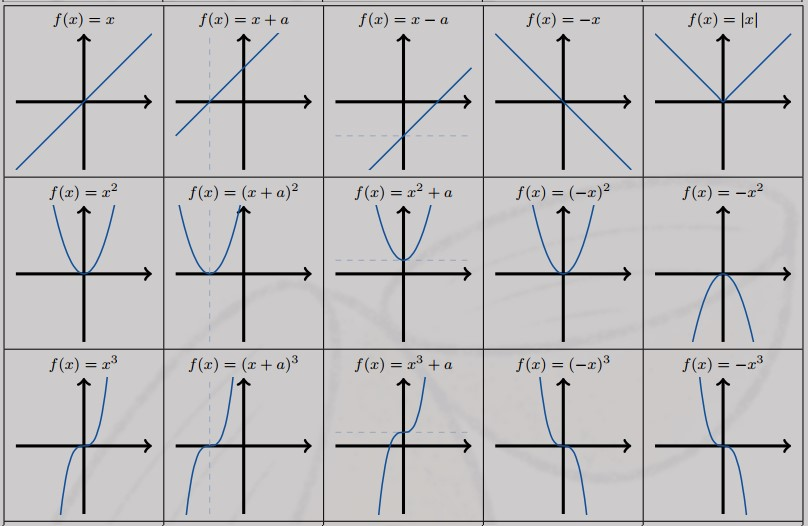
\includegraphics[width=15cm]{funciones_1}
	\caption{Funciones algebraicas}
	\label{funciones algebraicas1}
	
\end{figure}
	
	\begin{figure}[h]
	\centering
	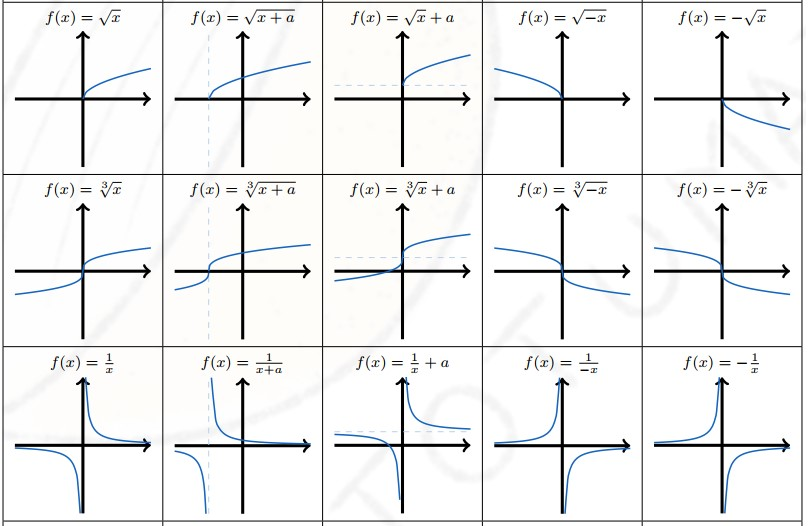
\includegraphics[width=15cm]{funciones_2}
	\caption{Funciones algebraicas}
	\label{funciones algebraicas2}
	\end{figure}
%%		
	\begin{figure}[h]
	\centering
	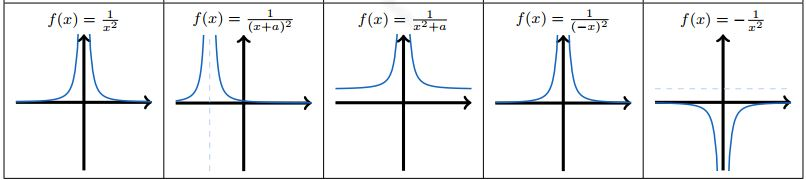
\includegraphics[width=15cm]{funciones_3}
	\caption{Funciones algebraicas}
	\label{funciones algebraicas3}
	\end{figure}
	
	

	\begin{figure}[h]
	\centering
	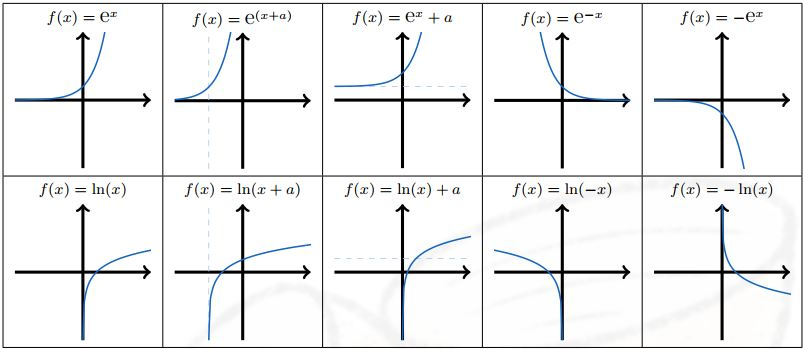
\includegraphics[width=15cm]{funciones_4}
	\caption{Funciones trascendentes}
	\label{Funciones_trascendentes}
	\end{figure}
%
%    \begin{figure}[h]
%	\centering
%	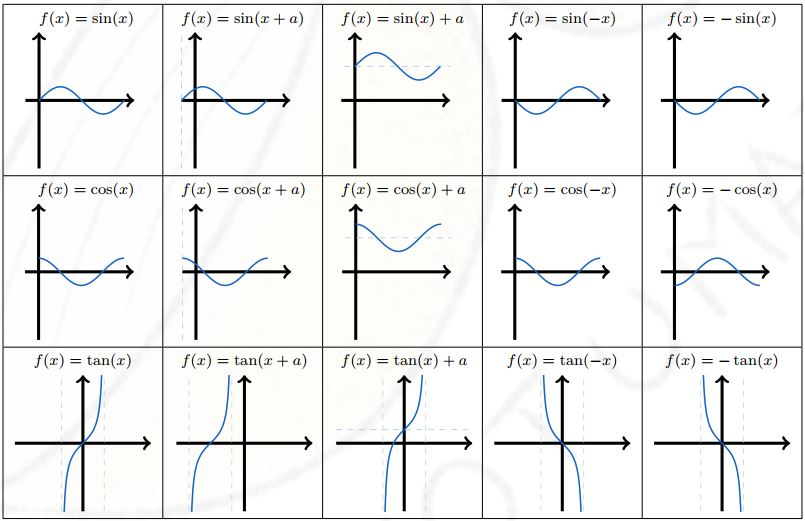
\includegraphics[width=15cm]{funciones_5}
%	\caption{Funciones trigonométricas}
%	\label{funciones trigonométricas}
%	\end{figure}
%%%%%%%%%%%%%%%%%%%%%%%%%%%%%%%%%%%%%%%%%%%%%%%%%%%%%%%%%%%%%%%%%%%%%%%%%%%%%%%%%%%%%%%%%%%%%%%%%%%%%%%%%%%%%%%%%%%%%%%%%%%%%%%%%%%%%%%%%%%%%%%%%%%%%%%%%%%%%%%%%%%%%%%%%%%%%%%%%%%%%%%%%%%%%%%%%%%%%%%%%%%%%%%%%%%%%%%%%%%%%%%%%%%%%%%%%%%%%%%%%%%%%%%%%%%%%%%%%%%%%%%%%%%%%%%%%%%%%%%%%%%%%%%%%%%%%%%%%%%%%%%%%%%%%%%%%%%%%%%%%%%%%%%%%%%%%%%%%%%%%%%%%%%%%%%%%%%%%%%%%%%%%%%%%%%%%%%%%%%%%%%%%%%%%%%%%%%%%%%%%%%%%%%%%%%%%%%%%%%%%%%%%%%%%%%%%%%%%%%%%%%%%%%%%%%%%%%%%%%%%%%%%%%%%%%%%%%%%%%%%%%%%%%%%%%%%%%%%%%%%%%%%%%%%%%%%%%%%%%%%%%%%%%%%%%%%%%%%%%%%%%%%%%%%%%%%%%%%%%%%%%%%%%%%%%%%%%%%%%%%%%%%%%%%%%%%%%%%%%%%%%%%%%%%%%%%%%%%%%%%%%%%%%%%%%%%%%%%%%%%%%%%%%%%%%%%%%%%%%%%%%%%%%%%%%%%%%%%%%%%%%%%%%%%%%%%%%%%%%%%%%%%%%%%%%%%%%%%%%%%%%%%%%%%%%%%%%%%%%%%%%%%%%%%%%%%%%%%%%%%%%%%%%%%%%%%%
%------------------------------------------------
%\phantomsection
%\section*{Acknowledgments} % The \section*{} command stops section numbering
%
%\addcontentsline{toc}{section}{Acknowledgments} % Adds this section to the table of contents
%
%So long and thanks for all the fish \cite{Figueredo:2009dg}.
%
%%----------------------------------------------------------------------------------------
%	REFERENCE LIST
%----------------------------------------------------------------------------------------
%\phantomsection
\newpage
\bibliographystyle{plain}
\bibliography{sample}

%%----------------------------------------------------------------------------------------

\end{document}